\documentclass[11pt]{article}

\usepackage[margin=1in]{geometry}
\usepackage{amsmath,amssymb,amsthm,mathtools}
\usepackage{booktabs,array}
\usepackage{graphicx}
\usepackage{float}
\usepackage{tikz}
\usetikzlibrary{arrows.meta,positioning}
\usepackage{microtype}
\usepackage{setspace}
\usepackage{needspace}
\usepackage{enumitem}
\usepackage[round,authoryear]{natbib}
\usepackage[colorlinks=true,allcolors=blue]{hyperref}

\newtheorem{proposition}{Proposition}
\newtheorem{definition}{Definition}
\newtheorem{assumption}{Assumption}
\newtheorem{remark}{Remark}
\theoremstyle{definition}
\newtheorem{conditionalresult}{Conditional result}

\newcommand{\dd}{\,\mathrm{d}}
\newcommand{\gA}{g_A}
\newcommand{\gY}{g_Y}
\newcommand{\gw}{g_w}
\newcommand{\sX}{s_X}
\newcommand{\sM}{s_M}
\newcolumntype{P}[1]{>{\raggedright\arraybackslash}p{#1}}

\title{The Future of Growth and Human Labor under Automated AI Research:\\
AI Capability as Research-Augmenting Technology}
\author{Oliver Pardo}
\date{August 2026}

\begin{document}
\maketitle

\begin{abstract}
I develop a decentralized endogenous-growth model in which AI capability makes
compute more productive in both final production and AI research. A monopolistic
developer supplies AI production services and invests in capability, creating a
feedback loop: better AI raises current output and also helps produce still better
AI. I study how this feedback affects economic growth, wages, interest rates, and
the distribution of income.

The results depend on how easily AI production services can replace labor. When
they are complements, labor remains a bottleneck: output per person and real wages
approach constants, and labor retains a positive income share even when AI research
services receive nearly all research expenditure. At unit elasticity, positive
balanced growth is possible only if the feedback remains below an explicit
threshold. When AI production services are gross substitutes for labor and
eventually dominate production, finite-rate balanced growth is impossible. Along
a conditional branch of the necessary conditions, output and the interest rate
become unbounded in finite time, while labor's income share converges to zero even
though the real wage rises.

The transition can nevertheless look uneventful for a long time before growth
accelerates sharply and labor's share collapses. Much of the displaced labor
income is absorbed by inference and research compute rather than becoming
developer profit. The explosive branch is a numerical illustration of the
model's necessary conditions, not an established infinite-horizon equilibrium.
\end{abstract}

\onehalfspacing

\section{Introduction}

The economic question is not only whether artificial intelligence can perform
tasks currently done by workers. It is also whether AI can perform the research
that produces better AI. When current AI capability determines the productivity
of compute used both in final production and in AI research, a familiar
substitution problem also creates a dynamic feedback. Following the useful
distinction in \citet{davidsonetal2026}, higher capability operates through two
loops. The technological loop raises the services produced by research compute;
the economic loop raises output and therefore the resources that can be devoted
to accumulation and research. Higher capability also lowers the resource cost of
a unit of AI service. The conditions under which this
feedback can settle into balanced growth or enter an accelerating branch depend
on substitution possibilities in both sectors, the strength of the resulting
feedback, and the branch that is reached.

This paper studies that feedback in a general-equilibrium growth model. Raw
compute has two uses. Inference compute is transformed by current AI capability
into services used in final production. AI R\&D compute---called research compute
below---is transformed by the same capability into automated research services.
Human researchers and automated research services are combined with a CES
technology to improve AI capability.
An integrated monopolist sells production services to final-good firms and uses
automated research services internally. The representative household owns capital
and the developer, supplies labor, and chooses consumption. Population grows
exogenously.

Research substitution and research scale are separate. The elasticity
\(\sigma_{HM}\) governs the response of the input mix to relative prices, whereas
\(0<\eta<1\) imposes decreasing returns to a proportional expansion of current
research inputs, holding capability fixed. The boundary \(\eta=1\) is substantive,
not a normalization. The baseline imposes the stronger restriction
\(\eta<\alpha\). Proposition \ref{prop:axm-research-burst} shows why. For all
positive CES elasticities, on any fixed horizon with regular positive price and
quantity paths, let \(S\) denote
total research expenditure. Capability is at most of order
\(1+S^{\eta/(1-\eta)}\), and optimized operating profit implies the bound
\[
 J_T\leq C_0+C_1S^{\eta(1-\alpha)/[\alpha(1-\eta)]}-cS.
\]
The exponent is below one exactly when \(\eta<\alpha\). The truncated
developer objective is then coercive over all nonnegative research policies,
and its supremum is finite. If both CES nests permit gross substitution and
\(\eta>\alpha\), a fixed-duration expansion of research compute makes the
truncated value unbounded. Extending each policy
with zero controls after the truncation date also makes the corresponding
infinite-horizon developer value unbounded under the stated extension conditions.
At equality, coefficients rather than exponents determine the leading term of
this family, and the boundary is not fully characterized. With
\((\alpha,\eta)=(0.33,0.20)\), the exponent equals 0.5076. This result does
not establish compactness of the control set, attainment of the supremum,
global optimality, infinite-horizon well-posedness, or equilibrium existence.

The distinction between raw compute and the services produced by compute is
central. A unit of compute is not a unit of intelligence. Current capability
determines what a given unit of hardware, energy, and datacenter time can produce.
We therefore write production services as the product of capability and inference
compute, and automated research services as the product of capability and research
compute. This capability-times-compute architecture is the one-capability analogue
of the AI-service accounting in \citet{davidsonetal2026}. It is also informed by
the richer distinction between inference output, training activity, algorithms,
and model capital in \citet{korinekmckelvey2026}. Our reduction is substantive:
one stock \(A\) combines model quality and algorithmic efficiency and augments
both uses of compute. Our term research compute corresponds to their broad
training-and-R\&D compute category. It includes pretraining, post-training,
experimentation, synthetic-data generation, automated algorithmic search, and
compute used by AI systems engaged in research.

The model deliberately excludes a separate power of the capability stock from its
baseline research technology. Better AI affects research only by making research
compute more productive. In the terminology of \citet{davidsonetal2026}, the
parameter governing returns to the current scale of research and the parameter
governing intertemporal idea difficulty are distinct. Our \(\eta\) is the former;
the baseline imposes \(b=1\) on the latter. A term such as \(A^{1-b}\) could make
that second margin free: holding the effective-research index fixed, any \(b>0\)
introduces the familiar ideas-getting-harder force in the growth rate of capability,
while \(1-b>0\) also gives the stock a positive level effect on \(\dot A\)
\citep{jones1995,davidsonetal2026}. Setting \(b=1\) removes this separate
level-stock term and isolates the feedback carried by automated research services.

\subsection{Empirical motivation}

Available data do not measure the objects at the center of the research block:
the relative use and contribution of human researchers and automated research
services. They do, however, provide
separate measures of raw compute, electricity use, and quality-adjusted AI output.
In the data cited below, both the physical resources devoted to AI and the
services obtained from those resources expand rapidly, with quality-adjusted
output rising faster. These measures motivate the distinction between raw compute
and AI services; they do not identify either substitution elasticity.

\citet{korinekmckelvey2026} estimate that U.S. AI compute expenditure rose from
\$36.9 billion in 2023 to \$219.2 billion in 2025, while raw compute capacity rose
from 1.09 million to 10.7 million H100-equivalent units of compute capacity, a measure normalized
to the computing capacity of an NVIDIA H100 accelerator. Over the same two years,
their quality-adjusted inference and training indexes increased by factors
of approximately 1,502 and 78. The quality-adjusted series are model-based
estimates assembled from sparse data and allocation assumptions, not
national-account aggregates. Their relevance here is conceptual: more compute and
more services per unit of compute are distinct margins.

\begin{figure}[t]
\centering
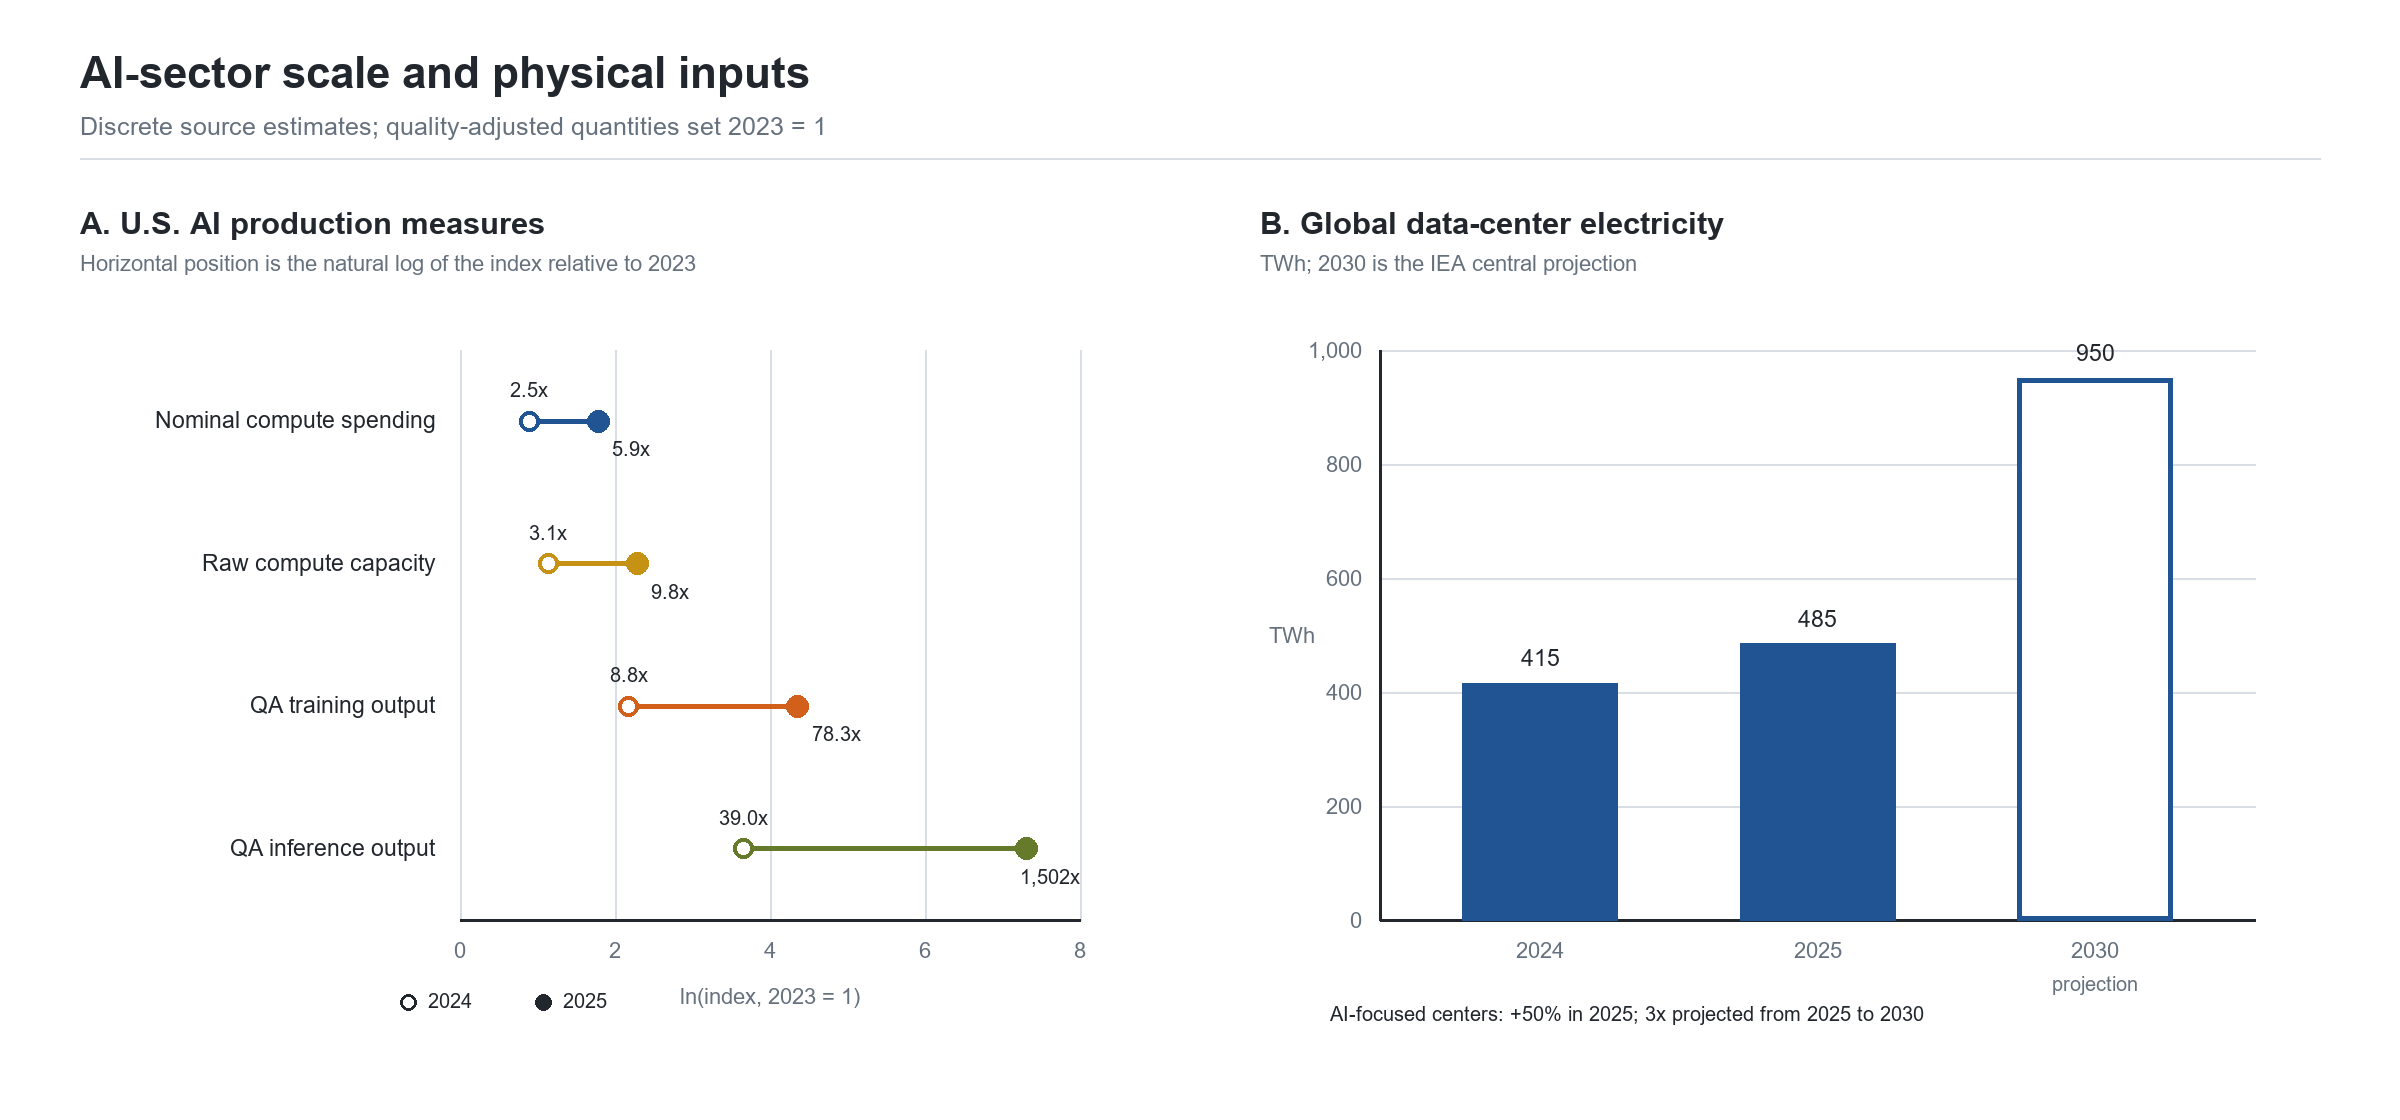
\includegraphics[width=\textwidth]{figures/empirical_ai_scale.png}
\caption{AI-sector scale and physical inputs. Panel A reports U.S. estimates for
2024 and 2025 relative to 2023; horizontal positions use natural logarithms because
the quality-adjusted quantities span several orders of magnitude. Panel B reports
IEA estimates of global data-center electricity use in 2024 and 2025 and its central
projection for 2030. Sources: \citet{korinekmckelvey2026}, \citet{iea2025}, and
\citet{iea2026}.}
\label{fig:axm-empirical-scale}
\end{figure}

Compute nevertheless remains a real resource. The International Energy Agency
estimates that global data-center electricity use rose from 415 TWh in 2024 to
485 TWh in 2025, and it projects approximately 950 TWh in 2030
\citep{iea2025,iea2026}. Normalizing the
common unit cost of inference and research compute therefore changes units; it
does not remove compute from the resource constraint.

Evidence closest to AI research automation comes from controlled evaluations. In
the original RE-Bench study, human experts with a 32-hour budget achieved almost
twice the average score of the best AI agent on machine-learning
research-engineering tasks \citep{metrrebench2024}. In a later evaluation on a
five-task subset, aggregating shorter Claude 3.7 runs to 32 hours produced a score
comparable to the median human score at eight hours \citep{metrclaude2025}.
These five tasks have unusually clear objectives and rapid feedback, and the model,
surrounding agent software and tools, tasks, and time budgets differ. The results
are therefore neither a comparable time series nor a measure of substitution in
real-world AI research. They
motivate the possibility of substitution in AI research without measuring
\(H/(AM)\) or \(\sigma_{HM}\).

The numerical exercises below are therefore scenarios rather than forecasts. The
evidence motivates the distinction between raw compute and service flows and the
two uses of compute, but it does not calibrate the feedback strength or the
conditions under which the economy reaches the accelerating branch.

\subsection{Results and contribution}

The analysis separates three regimes according to the elasticity of substitution
between labor and AI services in final production. When the elasticity is below
one, an interior complementarity limit satisfying the regularity conditions in
Proposition~\ref{prop:axm-complements} has a finite ratio of AI services to
production labor. Final output then becomes asymptotically proportional to a
Cobb--Douglas function of capital and production labor. On any finite-rate
balanced-growth path that satisfies the stated conditions and keeps production
labor at a positive population share, output per capita is constant. The audited
finite-horizon candidate paths make the distinction from research automation
visible: capability keeps growing in both reported complementarity cases, and
with substitutable research the automated research-expenditure share approaches
one. Over the same transition, output per person, consumption per person, and the
real wage move toward their conditional constant limits, while labor retains a
positive income share. At unit elasticity, the paper
derives the growth rates and resource shares of balanced-growth candidates. An
asymptotically automated research sector places greater weight on the feedback
from capability to both production and research and therefore tightens the
condition for positive balanced growth. When the final-production elasticity
exceeds one and AI services asymptotically dominate the labor--AI composite,
unbounded capability raises \(Y/K\) and the net interest rate without bound. A finite-rate
balanced-growth path is then impossible.

For the regime with gross substitution in both final production and AI research,
the paper goes beyond this nonexistence result.
It characterizes a conditional AI-dominated limiting branch of the necessary
conditions on which output, capital, consumption, and capability accelerate. The characterization assumes
that the path remains interior, converges to the postulated ratios, and satisfies
the monopoly second-order condition. Under those conditions,
aggregate labor income as a share of output tends to zero, while the real wage
rises when the smaller of the two substitution elasticities is below an explicit
threshold and falls when it is above that threshold. The distinction between labor income's
share of output and the wage level is economically important: a factor may
receive a vanishing fraction of an economy that is expanding even faster.

The complementarity and unit-elasticity computations solve the same dated
equilibrium system under the capability law used in the paper. The two reported
unit-elasticity parameterizations also satisfy the sufficient
concavity restrictions in Proposition \ref{prop:axm-equilibrium-sufficiency}.
Their numerical path approximations solve the household Euler equation, the developer's
research first-order conditions and costate equation, the monopoly pricing
condition, both market-clearing conditions, and the two laws of motion. The
simulations are used to illustrate propositions, not to replace them. The reported
paths are rejected unless all dated static, first-order, market, and dynamic
residuals are small and the monopoly second-order margin is positive. Finite
terminal conditions approximate, but do not prove, the infinite-horizon
transversality limits.

For gross substitution in final production, a separate free-boundary calculation
solves the necessary conditions up to successively larger values of \(Y/K\).
The resulting paths converge on common pre-singular intervals and their estimated
singularity dates converge. This is evidence for the conditional accelerating
branch, but not a proof of its global intertemporal optimality, reachability from
arbitrary initial states, or continuation beyond the finite-time boundary.

The closest analytical benchmark is \citet{davidsonetal2026}, who already
combine nonrival AI capability with rival compute and distinguish technological
from economic feedback in a multitechnology innovation network. This paper embeds
a one-capability version of that architecture in a decentralized Ramsey economy
with an integrated monopolist. Its contribution is to determine inference and
research compute, production and research labor, saving, prices, and factor shares
jointly rather than fixing the relevant allocation shares. The two CES margins
make the local link weights endogenous equilibrium objects determined jointly by
relative prices and allocations. In the
unit-elasticity regime, the balanced-growth denominator becomes the scalar analogue
of Davidson et al.'s feedback-matrix condition. In the conditional AI-dominated
limit, the model also derives an explicit threshold separating rising from falling
wages: the relevant elasticity is the smaller of the substitution elasticities in
final production and AI research. This result does not infer wage behavior from
labor income's share of output.

\section{Related literature}

The research technology belongs to the tradition of endogenous and
semi-endogenous growth models in which resources devoted to ideas determine the
evolution of productivity \citep{romer1990,aghionhowitt1992,jones1995}. The
population term matters for the same reason it matters in \citet{jones1995}: when
human researchers remain essential, growth in the research workforce can anchor
long-run innovation. I ask when that anchor disappears because
capability-augmented research services can substitute for human researchers. I use
a homothetic CES research technology to separate substitution between research
inputs from returns to their current joint scale. The latter role of \(\eta\) is analogous
to the intratemporal research-scale parameter in \citet{jones1995}; the baseline
fixes the separate stock-of-ideas exponent at zero, corresponding to \(b=1\) in
the extension discussed below.

The closest paper for the feedback architecture is \citet{davidsonetal2026}. They model innovation as a network
of technological and economic feedbacks, classify its growth regimes using the
spectral radius of a nonnegative feedback matrix, and combine nonrival AI
capability with rival compute. Their application distinguishes software, hardware
quality, and general productivity, but fixes saving and resource-allocation shares
and treats task automation as exogenous, including an exogenous path in its CES
extension. I collapse that technology network into one
capability stock and place its two feedback loops inside a decentralized Ramsey
equilibrium with an integrated monopolist, endogenous inference and research
compute, endogenous labor allocation, two CES substitution margins, and factor
prices. The mapping is not literal: in my formulation, \(U\) and \(M\) are flow
resource uses, not separate accumulable hardware stocks. The unit-elasticity
denominator in my model is therefore a scalar analogue of their
feedback criterion, not an application of their general network theorem.

The large-scale curvature restriction derived below answers a different
question from \citet{davidsonetal2026}'s feedback criterion. Their matrix
criterion classifies a coupled system of technological and economic feedbacks.
Davidson et al.'s matrix criterion concerns the propagation of feedback through
a coupled growth system. By contrast, \(\eta<\alpha\) rules out a particular
unbounded-value deviation in the developer's problem. Neither condition, by
itself, proves equilibrium existence.

I also relate the model to broader work on AI and economic growth.
\citet{aghionjonesjones2019} show how extending automation to idea production can
generate very rapid growth, while essential tasks that remain difficult to
automate can preserve bottlenecks; they use ``singularity'' for a finite-time
divergence. \citet{nordhaus2021} develops empirical diagnostics for an economic
singularity, while \citet{trammellkorinek2023} distinguishes the automation of
ordinary production from the automation of R\&D in a model of transformative AI.
\citet{jones2025rd} focuses directly on AI in research and development.
\citet{erdiletal2025gate} integrate a compute-based model of AI development, an
AI-automation block, and semi-endogenous growth with endogenous investment and
adjustment costs in a quantitative scenario model that abstracts from market
prices and market structure. Relative to these papers, I focus more narrowly on
how equilibrium prices and two factor-substitution margins govern the feedback,
the allocation of compute, and the distribution of output.

The terminology used to distinguish inference output, training activity,
algorithms, and model capital is informed by the economic accounting proposed by
\citet{korinekmckelvey2026}. Their framework treats compute as a central input
allocated between inference and training/R\&D and separates model capital from
algorithmic advances. In my reduced notation, raw inference compute and raw
research compute are paid uses of final output, while one capability stock
transforms both into economically useful services. Thus \(A\) combines objects
that their accounting keeps separate. This is a tractability assumption, not an
exact relabeling of their framework. I use their measurement distinctions; the
decentralized equilibrium and distributional results below do not follow from
that accounting framework.

The final-production block connects to the older literature on the elasticity of
substitution and growth \citep{pitchford1960,jonesmanuelli1990,rebelo1991}. CES
production is not a cosmetic generalization of Cobb--Douglas: whether the
elasticity lies below or above one governs whether labor remains a bottleneck or
AI services can asymptotically dominate along the paths studied here. Empirical work such as
\citet{duffypapageorgiou2000} illustrates why the aggregate elasticity should not
be imposed without scrutiny. \citet{aumshin2024} sharpen this point by estimating
complementarity between equipment and labor but gross substitution between
software and labor. Their estimates do not calibrate the model's AI-service elasticity,
but they support separating software-like inputs from undifferentiated physical
capital.
\citet{jonestonetti2026} provide a task-based counterpart to the model's
complementarity regime. With an elasticity of substitution below one across
tasks, the remaining tasks performed by slowly improving labor act as weak links
and delay the growth acceleration even when most tasks have been automated.
Their simulated aggregate paths under endogenous automation can remain difficult
to distinguish for a long interval before their growth rates diverge sharply. This is the closest
dynamic precedent for the delayed takeoff in my finite-boundary calculations.
An earlier illustration in \citet{aghionjonesjones2019} likewise shows that
bottlenecks can sustain relatively low aggregate growth while automation
continues, although their numerical automation path is exogenous.
Jones and Tonetti's simulations also show that automation alone does not determine the
limiting factor shares: the capital share can rise to one under complete
automation, fall toward zero when some weak links can never be automated, or
remain approximately stable along an intermediate path. The analogy is not an
identity. Their elasticity aggregates tasks and automation changes the set of
tasks assigned to capital; the model's \(\sigma_{XL}\) aggregates production labor and a
flow of quality-adjusted AI services.
The complementarity result adds an endogenous-research margin to this older CES
logic. \citet{davidsonetal2026} also show why, under CES aggregation, the relevant
object is the current elasticity of the appropriate aggregate with respect to its
AI input rather than a raw count of automated tasks. In my model,
\(s_X=\partial\ln Z/\partial\ln X\) and
\(s_M=\partial\ln E/\partial\ln(AM)\) play that role within
the two CES aggregators; the corresponding downstream elasticities are
\((1-\alpha)s_X\) for final output and \(\eta s_M\) for capability improvement.
Davidson et al. provide the closer analogue for feedback amplification and its
explosive-growth threshold, not for the endogenous timing of the low-growth
phase: their quantitative exercise imposes an automation change and fixes the
relevant research-resource shares. The simulated dates reported in those papers
are therefore not transferable to this economy.
These objects are endogenous CES shares rather than fractions of tasks. The adjustment is
also different: on the complementary-input branch I characterize, monopoly supply
keeps \(X/L\) finite and \(s_X\) positive while the raw-compute cost \(U=X/A\)
vanishes. On the regular complementary-input balanced-growth limit characterized
here, capability can continue to improve and research expenditure can become
almost fully automated while labor remains essential, output and consumption per
person remain bounded, and labor retains a positive income share.

The wage and factor-share results relate to the task and automation literature.
\citet{acemoglurestrepo2019} emphasize displacement and reinstatement of labor in
a task framework, and \citet{acemoglu2025} studies the macroeconomic gains from AI
through task exposure. That literature distinguishes tasks---units of work used
in production---from jobs, which bundle several tasks. Automation can therefore
change the tasks performed within a job without eliminating the job itself. My
model abstracts from task content, occupations, and the creation of new human
tasks. Labor is an aggregate input and full employment holds by construction.
The results should therefore be interpreted as model implications for wages,
factor shares, and sectoral labor allocation, not as predictions about the number
of jobs displaced. Within that abstraction, the model shows how a wage can rise
even when labor income as a share of output falls because the scale of output
changes endogenously.
This mechanism is related to the distinction between wages and labor income shares
emphasized by \citet{autorkausik2026}, but here it is generated by AI research
feedback and monopoly supply. \citet{trammellkorinek2023} likewise show that wages
can rise or fall when output expands and labor income as a share of output contracts. The conditional
AI-dominated limit I characterize maps that ambiguity into an explicit threshold for the
smaller of the substitution elasticities in final production and AI research.

\citet{restrepo2025agi} provides the closest antecedent to the limiting
distributional mechanism. When compute can perform all bottleneck work and
computational resources expand, output becomes linear in compute and labor,
growth is driven by compute, and labor's income share converges to zero. That
paper establishes the broad possibility that removing the human bottleneck can
make labor asymptotically inessential for aggregate growth. Taken together,
\citet{restrepo2025agi}, \citet{acemoglurestrepo2019}, and
\citet{trammellkorinek2023} establish both the displacement mechanism and the
possibility of a vanishing labor share. I claim neither as new.

My contribution is to place related mechanisms in a different
decentralized architecture and characterize their associated prices and
allocations under the hypotheses of each regime. The two CES elasticities
determine whether human labor remains a production or research bottleneck; the
integrated developer links the same capability stock to inference revenue and
research investment; and the consolidated accounts separate gross capital
payments, production and research wages, distributed developer profit, inference
compute, and research compute along the transition. This decomposition also
limits its own interpretation. Inference and research compute are resource uses,
not final income recipients. Without an upstream compute sector, the model cannot
determine whether the associated payments accrue to hardware producers, energy
suppliers, workers, or owners of additional capital.

Finally, the integrated developer connects the analysis to the emerging literature
on AI market structure \citep{korinekvipra2025,gans2024,demireretal2025}. Monopoly
and integration enter through separate channels: the developer charges a markup
on production AI services and internalizes the future operating profits created
by better capability. I hold market structure fixed in order to isolate the
technology. Comparing this
benchmark with monopolistic competition is a natural next step.

\section{Model}
\label{sec:axm-model}

Time is continuous, and I suppress time subscripts except where they are needed
for clarity. There is one final good, a representative household, competitive
final-good firms, and an integrated AI developer. Two productivity indexes enter
the model. Labor productivity \(A\) grows exogenously. AI capability \(B\) is
produced endogenously by the developer. The developer monopolistically supplies
AI production services and invests in better AI. The initial economy already
uses AI production services; the model does not describe their first commercial
adoption.

I first present a benchmark in which AI research services are the only input
used to improve AI capability. This benchmark represents an economy in which
the replacement of human researchers in frontier AI development has already
occurred. I then introduce human research as an extension. This order separates
the mechanism needed for the main results from the additional mechanism that
affects the timing of the transition.

\tikzset{
 axm-model-input/.style={draw, rounded corners=2pt, minimum width=2.7cm,
  minimum height=1.0cm, align=center, fill=gray!8},
 axm-model-state/.style={draw, rounded corners=2pt, minimum width=2.7cm,
  minimum height=1.0cm, align=center, fill=blue!8},
 axm-model-technology/.style={draw, rounded corners=2pt, minimum width=3.5cm,
  minimum height=1.0cm, align=center, fill=orange!9},
 axm-model-problem/.style={draw, rounded corners=2pt, minimum height=1.2cm,
  align=center, fill=gray!6, text width=10.8cm},
 axm-model-flow/.style={->, semithick},
 axm-model-dynamics/.style={->, semithick, dashed}
}

\subsection{Population, labor endowment, and labor productivity}

Population grows exogenously at the constant rate \(n>0\):
\begin{equation}
 \dot N=nN.
 \label{eq:axm-population}
\end{equation}
Each person supplies one unit of homogeneous labor inelastically, so the
household supplies \(N\) units at the common wage \(w\). In the benchmark, all
labor is used in final production. The extension later allows the AI developer
to hire part of the labor endowment for research.

The variable \(A\) measures labor-augmenting productivity in final production.
One unit of production labor supplies \(A\) efficiency units, so effective
production labor is \(AL\). Labor productivity follows the exogenous law
\begin{equation}
 \dot A=\gamma_A A,
 \qquad \gamma_A\geq0,
 \label{eq:axm-labor-productivity}
\end{equation}
with \(A(0)>0\). The case \(\gamma_A=0\) nests the specification without
conventional labor-productivity growth. For any positive variable \(V\), write
\(g_V\equiv\dot V/V\); hence \(g_A=\gamma_A\).

\subsection{Household}

The representative household discounts utility at rate \(\rho>n\). It takes the
paths of the net interest rate \(r\), the wage \(w\), distributed developer
profit \(\Pi\), and population \(N\) as given. Let \(K\) denote its holdings of
physical capital. Given \(K(0)>0\), it chooses \(C\) and \(K\) to maximize
\[
 \int_0^\infty e^{-\rho t}N_t\log(C_t/N_t)\,\dd t.
\]
It owns physical capital and the AI developer and receives labor income, the net
return on capital, and distributed profit. Its flow budget is
\begin{equation}
 \dot K=rK+wN+\Pi-C.
 \label{eq:axm-household-budget}
\end{equation}
The variable \(r\) is the net real interest rate: depreciation is already
deducted from the rental return to capital. At this stage, \(r\) is a price the
household takes as given; no production-side condition has yet been imposed. The
household's interior Euler equation in aggregate variables is therefore
\begin{equation}
 \frac{\dot C}{C}=n+r-\rho.
 \label{eq:axm-euler}
\end{equation}
The infinite-horizon terminal restriction maintained for the household is
\begin{equation}
 \lim_{t\to\infty}e^{-\rho t}\frac{N_tK_t}{C_t}=0.
 \label{eq:axm-household-tvc}
\end{equation}

\subsection{Final-good firms}

Competitive final-good firms take \(r,w,p_X\) as given and demand capital,
production labor, and AI production services, where \(p_X\) is their price. To
preserve the notation used in the analysis and numerical code, I do not give
\(K\) and \(X\) agent-specific superscripts. In this subsection they denote
capital and AI production services demanded by the final sector; in the
household problem \(K\) denotes capital holdings, and in the developer's problem
\(X\) denotes sales. Equality of the corresponding quantities is imposed only
in equilibrium.

Let \(0<\alpha<1\) be the physical-capital elasticity, let \(\delta\geq0\) be
the depreciation rate, and let \(\sigma_{XL}>0\) be the elasticity of
substitution between effective production labor and AI production services. The
CES weights satisfy \(\omega_L,\omega_X\in(0,1)\) and
\(\omega_L+\omega_X=1\). The production technology is
\begin{align}
 Y&=K^\alpha Z^{1-\alpha},\\
 Z&=\left[\omega_L (AL)^{\frac{\sigma_{XL}-1}{\sigma_{XL}}}
 +\omega_X X^{\frac{\sigma_{XL}-1}{\sigma_{XL}}}\right]^{
 \frac{\sigma_{XL}}{\sigma_{XL}-1}},
 \qquad \omega_L+\omega_X=1.
 \label{eq:axm-final-production}
\end{align}
At the unit-elasticity limit, \(\sigma_{XL}\to1\), the CES becomes
\(Z=(AL)^{\omega_L}X^{\omega_X}\). Define the contribution of AI production
services to the CES quantity index as
\begin{equation}
 s_X=\frac{\omega_X X^{(\sigma_{XL}-1)/\sigma_{XL}}}
 {\omega_L (AL)^{(\sigma_{XL}-1)/\sigma_{XL}}
 +\omega_X X^{(\sigma_{XL}-1)/\sigma_{XL}}}.
 \label{eq:axm-sx}
\end{equation}
Thus \(s_X\) is the elasticity of \(Z\) with respect to \(X\). The competitive
sector solves
\begin{equation}
 \max_{K,L,X\geq0}\left\{K^\alpha Z(AL,X)^{1-\alpha}
 -(r+\delta)K-wL-p_XX\right\}.
 \label{eq:axm-final-firm-problem}
\end{equation}
The interior first-order conditions are
\begin{equation}
 r=\alpha\frac{Y}{K}-\delta,\qquad
 w=(1-\alpha)(1-s_X)\frac{Y}{L},\qquad
 p_X=(1-\alpha)s_X\frac{Y}{X}.
 \label{eq:axm-factor-prices}
\end{equation}
Labor productivity \(A\) affects the wage through \(Y\) and \(s_X\). It does
not appear as an additional factor in the wage equation because \(AL\) is
linear in \(L\), so the output elasticity with respect to \(L\) equals the
elasticity with respect to effective labor \(AL\).

To ask how an expansion of AI production services affects production labor,
holding \(K\) fixed is not enough: either the wage or labor must also be held
fixed. I therefore state both sides of the same comparative static. The
conditional labor-demand response holds \(K\), \(A\), and \(w\) fixed; the dual
wage response holds \(K\), \(A\), and \(L\) fixed. The distinction between the
wage and labor-share responses follows the general result in
\citet[Theorem~1]{autorkausik2026}. For this nested Cobb--Douglas--CES
technology, \citet[Proposition~2.2, Appendix~A.4, Lemma~4.1, and
Proposition~4.2]{yango2026} derive the corresponding labor-demand sign and the
two elasticity thresholds.

Define production labor's share of final output as
\begin{equation}
 \ell^Y\equiv\frac{wL}{Y}=(1-\alpha)(1-s_X).
 \label{eq:axm-production-labor-share}
\end{equation}

\Needspace{24\baselineskip}
\begin{proposition}[AI services and production labor]
\label{prop:axm-ai-labor-comparative-static}
For an interior final-good firm, an increase in \(X\), holding \(K\), \(A\),
and \(L\) fixed, satisfies
\begin{align}
 \left.\frac{\partial\ln Y}{\partial\ln X}\right|_{K,A,L}
 &=(1-\alpha)s_X>0,
 \label{eq:axm-output-x-elasticity}\\
 \left.\frac{\partial\ln w}{\partial\ln X}\right|_{K,A,L}
 &=\left(\frac{1}{\sigma_{XL}}-\alpha\right)s_X,
 \label{eq:axm-wage-x-elasticity}\\
 \left.\frac{\partial\ln \ell^Y}{\partial\ln X}\right|_{K,A,L}
 &=-\left(1-\frac{1}{\sigma_{XL}}\right)s_X.
 \label{eq:axm-labor-share-x-elasticity}
\end{align}
Equivalently, holding \(K\), \(A\), and \(w\) fixed, conditional
production-labor demand satisfies
\begin{equation}
 \left.\frac{\partial\ln L}{\partial\ln X}\right|_{K,A,w}
 =\frac{s_X\left(\sigma_{XL}^{-1}-\alpha\right)}
 {\alpha(1-s_X)+s_X/\sigma_{XL}}.
 \label{eq:axm-labor-demand-x-elasticity}
\end{equation}
Thus an expansion of AI production services raises conditional labor demand---or,
at fixed labor, raises the wage---if and only if
\(\sigma_{XL}<1/\alpha\). It lowers conditional labor demand and the wage if and
only if \(\sigma_{XL}>1/\alpha\). By contrast, production labor's share falls if
and only if \(\sigma_{XL}>1\). Since \(0<\alpha<1\), the interval
\begin{equation}
 1<\sigma_{XL}<\frac{1}{\alpha}
 \label{eq:axm-wage-share-decoupling-region}
\end{equation}
is nonempty: within it, more AI production services raise labor demand at a
given wage, and raise the wage at a given employment level, even as labor
receives a smaller share of output.
\end{proposition}

\begin{proof}
The CES share in \eqref{eq:axm-sx} implies
\[
 \left.\frac{\partial\ln(1-s_X)}{\partial\ln X}\right|_{A,L}
 =-\left(1-\frac{1}{\sigma_{XL}}\right)s_X.
\]
The output elasticity in \eqref{eq:axm-output-x-elasticity} follows directly
from \eqref{eq:axm-final-production}. Combining these two elasticities with the
wage equation in \eqref{eq:axm-factor-prices} gives
\eqref{eq:axm-wage-x-elasticity}; combining the share equation above with
\eqref{eq:axm-production-labor-share} gives
\eqref{eq:axm-labor-share-x-elasticity}. Finally,
\[
 \left.\frac{\partial\ln w}{\partial\ln L}\right|_{K,A,X}
 =-\left[\alpha(1-s_X)+\frac{s_X}{\sigma_{XL}}\right]<0.
\]
Implicit differentiation of the labor-demand condition at fixed \(w\) gives
\eqref{eq:axm-labor-demand-x-elasticity}. Its denominator is strictly positive,
so its sign is the sign of \(\sigma_{XL}^{-1}-\alpha\). The remaining sign
statements follow from the displayed elasticities.
\end{proof}

The final-good firm's AI-demand condition implies
\(p_XX/Y=(1-\alpha)s_X\). After market clearing, this is the developer's gross
service revenue as a share of final output. Constant returns and the three
first-order conditions imply zero profit:
\begin{equation}
 Y=(r+\delta)K+wL+p_XX.
 \label{eq:axm-final-zero-profit}
\end{equation}
Solving the AI-demand condition for its price yields the inverse demand schedule
\(p_X(X;K,A,L)\). Define its inverse absolute elasticity as
\begin{equation}
 \varepsilon_X^{-1}
 \equiv-\left.\frac{\partial\ln p_X(X;K,A,L)}{\partial\ln X}\right|_{K,A,L}
 =\frac{1-s_X}{\sigma_{XL}}+\alpha s_X.
 \label{eq:axm-inverse-elasticity}
\end{equation}

\begin{remark}[Tasks, jobs, and labor services]
The input \(L\) is a quantity of homogeneous labor services, not a number of
tasks, occupations, or jobs. The benchmark imposes full employment in final
production. The extension allows workers to move between production and
research. Neither version describes unemployment or the number of tasks
displaced by AI.
\end{remark}

\subsection{Integrated AI developer: automated-research benchmark}

\subsubsection{AI production and research services}

The model distinguishes two uses of compute. \(U\) is inference compute: raw
compute used to operate existing AI systems and supply services to final-good
firms. \(M\) is AI R\&D compute---called research compute below---used to improve
AI capability. Both are flows rather than stocks of chips, and both have the
same constant unit resource cost. I choose units so that one unit of raw compute
costs one unit of final output.

The stock \(B\) indexes current AI capability: what one unit of compute can
accomplish. Inference compute produces the flow of AI production services
\begin{equation}
 X=BU.
 \label{eq:axm-ai-service}
\end{equation}
Research compute analogously produces the flow of AI research services \(BM\).
The paid inputs are \(U\) and \(M\), whereas \(X\) and \(BM\) are service flows.
This product of nonrival capability and rival compute is the one-capability
version of the capability--compute accounting in \citet{davidsonetal2026}.
Producing one unit of either service flow uses \(1/B\) units of final output.

Figure~\ref{fig:axm-current-production-flow} collects the current-production
technology. Gray boxes denote current inputs, blue boxes denote stocks, and
orange boxes denote transformations or outputs. The diagram is a schematic,
not a numerical result.

\begin{figure}[H]
 \centering
 \resizebox{0.90\textwidth}{!}{%
 \begin{tikzpicture}[>=Latex,font=\small]
  \node[axm-model-state]      (B) at (-8.0,-0.2) {\(B\)\\AI capability};
  \node[axm-model-input]      (U) at (-8.0,-1.6) {\(U\)\\inference compute};
  \node[axm-model-technology] (X) at (-4.5,-0.9)
   {\(X=BU\)\\AI production services};
  \node[axm-model-state]      (A) at (-8.0, 2.7) {\(A\)\\labor productivity};
  \node[axm-model-input]      (L) at (-8.0, 1.3)
   {\(L\)\\production labor};
  \node[axm-model-technology] (AL) at (-4.5, 2.0)
   {\(AL\)\\effective labor};
  \node[axm-model-technology] (Z) at ( 0.0, 0.8)
   {\(Z=\operatorname{CES}(AL,X)\)\\elasticity \(\sigma_{XL}\)};
  \node[axm-model-state]      (K) at ( 0.0, 3.7)
   {\(K\)\\physical capital};
  \node[axm-model-technology] (Y) at ( 4.0, 2.5)
   {\(Y=K^\alpha Z^{1-\alpha}\)\\final output};

  \draw[axm-model-flow] (B) -- (X);
  \draw[axm-model-flow] (U) -- (X);
  \draw[axm-model-flow] (A) -- (AL);
  \draw[axm-model-flow] (L) -- (AL);
  \draw[axm-model-flow] (AL) -- (Z);
  \draw[axm-model-flow] (X) -- (Z);
  \draw[axm-model-flow] (Z) -- (Y);
  \draw[axm-model-flow] (K) -- (Y);
 \end{tikzpicture}%
 }
 \caption{Current production. Labor productivity and production labor produce
 effective labor \(AL\). AI capability and inference compute produce AI
 production services \(X\). Effective labor and AI production services form the
 CES composite \(Z\), which combines with physical capital to produce final
 output.}
 \label{fig:axm-current-production-flow}
\end{figure}

\subsubsection{Capability accumulation}

In the benchmark, AI research services are the only input used to improve
capability:
\begin{equation}
 \dot B=\chi(BM)^\eta,
 \qquad \chi>0,\quad 0<\eta<1.
 \label{eq:axm-capability-law-benchmark}
\end{equation}
The scalar \(\chi\) shifts research productivity. The exponent \(\eta\) governs
returns to current research scale: for a fixed \(B\), multiplying \(M\) by
\(\lambda\) multiplies \(\dot B\) by \(\lambda^\eta\). Capability enters only
through \(BM\), so the benchmark has no separate \(B^\phi\) term. Better
capability makes each unit of research compute more productive, while \(\eta\)
governs decreasing returns to the current flow of research compute.

\begin{figure}[H]
 \centering
 \resizebox{0.78\textwidth}{!}{%
 \begin{tikzpicture}[>=Latex,font=\small]
  \node[axm-model-state]      (B)  at (-5.7, 1.2)
   {\(B\)\\AI capability};
  \node[axm-model-input]      (M)  at (-5.7,-1.2)
   {\(M\)\\research compute};
  \node[axm-model-technology] (BM) at (-1.7, 0.0)
   {\(BM\)\\AI research services};
  \node[axm-model-technology] (Bd) at ( 3.2, 0.0)
   {\(\dot B=\chi(BM)^\eta\)\\new capability};

  \draw[axm-model-flow] (B) -- (BM);
  \draw[axm-model-flow] (M) -- (BM);
  \draw[axm-model-flow] (BM) -- (Bd);
  \draw[axm-model-dynamics] (Bd.east) -- (5.2,0.0) -- (5.2,2.8) --
   node[above] {capability accumulation} (-5.7,2.8) -- (B.north);
 \end{tikzpicture}%
 }
 \caption{AI research in the benchmark. Capability and research compute produce
 AI research services \(BM\). Those services improve capability, and the new
 capability stock raises the productivity of subsequent research compute.}
 \label{fig:axm-research-flow}
\end{figure}

\subsubsection{Dynamic problem}

The developer sells \(X\), pays \(X/B\) for inference compute, uses \(M\) for
research, and owns \(B\). It faces the inverse demand schedule derived from
final-good firms' optimal demand. Taking the paths of \(r,K,A,\) and \(L\) as
given, it solves
\begin{equation}
 \max_{\{X,M\}}
 \int_0^\infty
 \exp\left\{-\int_0^t r_s\dd s\right\}
 \left[p_X(X_t;K_t,A_t,L_t)X_t-\frac{X_t}{B_t}-M_t\right]\dd t,
 \label{eq:axm-developer-problem-benchmark}
\end{equation}
subject to \eqref{eq:axm-capability-law-benchmark} and the initial capability
stock. The discount rate is the market return available to the household that
owns the developer. Equilibrium later requires consistency between this return,
household saving, and final-good firms' capital demand. The developer's
instantaneous distributed profit is
\begin{equation}
 \Pi=p_X(X;K,A,L)X-\frac{X}{B}-M=p_XX-U-M.
 \label{eq:axm-developer-profit-benchmark}
\end{equation}
This net payout can be negative. The model imposes no separate cash-flow or
borrowing constraint, so a negative \(\Pi\) represents an equity injection from
the household that owns the developer.

Sales \(X\) do not enter the capability law or another intertemporal constraint,
and there is no firm-level capacity constraint linking \(U\) and \(M\). The
developer therefore chooses \(X\) pointwise, while \(M\) affects future
capability. Conditional on current \(B,K,A,\) and \(L\), optimized operating
profit before research expenditure is
\begin{equation}
 \pi(B;K,A,L)=\max_{X\geq0}
 \left\{p_X(X;K,A,L)X-\frac{X}{B}\right\}.
 \label{eq:axm-service-supply}
\end{equation}
On an interior monopoly branch, the first-order condition is
\begin{equation}
 p_X(1-\varepsilon_X^{-1})=\frac{1}{B}.
 \label{eq:axm-monopoly-foc}
\end{equation}
Writing \(e_X=\varepsilon_X^{-1}\), the strict second-order condition is
\begin{equation}
 e_X(1-e_X)
 +(\alpha-\sigma_{XL}^{-1})(1-\sigma_{XL}^{-1})s_X(1-s_X)>0.
 \label{eq:axm-monopoly-soc}
\end{equation}

Whenever the pointwise maximum is attained, the primitive problem is equivalent
to
\begin{equation}
 \max_{\{M\}}
 \int_0^\infty
 \exp\left\{-\int_0^t r_s\dd s\right\}
 \left[\pi(B_t;K_t,A_t,L_t)-M_t\right]\dd t,
 \label{eq:axm-developer-problem-reduced-benchmark}
\end{equation}
subject to the same capability law and initial stock. The maximization over
\(X\) is therefore the pointwise inner maximization of one dynamic problem, not
a second decision problem.

\begin{figure}[H]
 \centering
 \begin{tikzpicture}[>=Latex,font=\small,node distance=1.25cm]
  \node[axm-model-problem] (full) {
   \textbf{Primitive dynamic problem, \eqref{eq:axm-developer-problem-benchmark}}\\
   choose \(X,M\); state \(B\); flow payoff
   \(p_X(X;K,A,L)X-X/B-M\)};
  \node[axm-model-problem, below=of full, fill=orange!9] (inner) {
   \textbf{Pointwise inner choice, \eqref{eq:axm-service-supply}}\\
   \(\displaystyle \pi(B;K,A,L)=\max_{X\geq0}
   \{p_X(X;K,A,L)X-X/B\}\)};
  \node[axm-model-problem, below=of inner, fill=blue!8] (reduced) {
   \textbf{Equivalent reduced dynamic problem,
   \eqref{eq:axm-developer-problem-reduced-benchmark}}\\
   choose \(M\); same state law and initial \(B\); flow payoff
   \(\pi(B;K,A,L)-M\)};

  \draw[axm-model-flow] (full) -- node[right,align=left]
   {\(X\) does not enter \(\dot B\) or another\\intertemporal constraint}
   (inner);
  \draw[axm-model-flow] (inner) -- node[right]
   {substitute optimized operating profit} (reduced);
 \end{tikzpicture}
 \caption{Decomposition of the developer's benchmark problem. The maximization
 over \(X\) is an inner, within-date choice. Substituting optimized operating
 profit leaves the dynamic choice of research compute \(M\).}
 \label{fig:axm-developer-decomposition}
\end{figure}

\subsubsection{Dynamic optimality}

Let \(q\) be the current-value shadow price of AI capability. The interior
first-order condition for research compute is
\begin{equation}
 q\chi\eta B(BM)^{\eta-1}=1.
 \label{eq:axm-research-foc-benchmark}
\end{equation}
Equivalently,
\begin{equation}
 M=\left(q\chi\eta B^\eta\right)^{1/(1-\eta)}.
 \label{eq:axm-research-demand-benchmark}
\end{equation}
This expression determines current research compute after \(B\) and \(q\) are
known. It is derived from the developer's problem and is not an additional
resource constraint.

The envelope theorem applied to \eqref{eq:axm-service-supply} gives
\(\pi_B=X/B^2\). Holding \(M\) fixed, the capability law gives
\(\partial\dot B/\partial B=\eta\dot B/B\). The current-value costate equation is
therefore
\begin{equation}
 \frac{\dot q}{q}=r-\frac{X}{qB^2}-\eta\frac{\dot B}{B}.
 \label{eq:axm-costate-benchmark}
\end{equation}
The infinite-horizon terminal restriction maintained for the developer is
\begin{equation}
 \lim_{t\to\infty}
 \exp\left\{-\int_0^t r_s\dd s\right\}q_tB_t=0.
 \label{eq:axm-developer-tvc}
\end{equation}

\subsection{Benchmark equilibrium}

Capital-market clearing requires the household's capital holdings to equal the
capital rented by final-good firms. Market clearing for AI production services
requires the quantity purchased by final-good firms to equal the quantity sold
by the developer. Labor-market clearing in the benchmark imposes
\begin{equation}
 N=L.
 \label{eq:axm-labor-market-benchmark}
\end{equation}

Substituting developer profit \eqref{eq:axm-developer-profit-benchmark}, labor-
market clearing, and market clearing for AI production services into the
household budget gives
\[
 \dot K=rK+wL+p_XX-U-M-C.
\]
Using the final sector's zero-profit identity yields the aggregate resource
constraint
\begin{equation}
 C+\dot K+\delta K+U+M=Y.
 \label{eq:axm-resource}
\end{equation}
The corresponding accounting decomposition is
\begin{align}
 Y&=(r+\delta)K+wL+\Pi+U+M,\notag\\
 1&=\frac{(r+\delta)K}{Y}+\frac{wL}{Y}
 +\frac{\Pi}{Y}+\frac{U}{Y}+\frac{M}{Y}.
 \label{eq:axm-consolidated-distribution-benchmark}
\end{align}
This identity separates the gross capital payment, labor income, distributed
developer profit, inference compute, and research compute. It is an accounting
consequence of equilibrium, not an additional restriction.

Only after market clearing can conditions from different agents be combined.
The household Euler equation and the final-good firm's capital demand imply
\begin{equation}
 \frac{\dot C}{C}=n+\alpha\frac{Y}{K}-\delta-\rho.
 \label{eq:axm-euler-reduced}
\end{equation}
Substituting the same capital-price condition into the developer's costate
equation gives
\begin{equation}
 \frac{\dot q}{q}=\alpha\frac{Y}{K}-\delta-
 \frac{X}{qB^2}-\eta\frac{\dot B}{B}.
 \label{eq:axm-costate-reduced-benchmark}
\end{equation}

The benchmark contains a technological loop,
\(B\to BM\to\dot B\to B\), and an economic loop,
\(B\to X\to Y\to(K,M)\to BM\to\dot B\to B\). Three local elasticities
summarize the direct technological links:
\begin{equation}
 \left.\frac{\partial\ln X}{\partial\ln B}\right|_U=1,\qquad
 \left.\frac{\partial\ln Y}{\partial\ln X}\right|_{K,A,L}
 =(1-\alpha)s_X,\qquad
 \frac{\partial\ln\dot B}{\partial\ln(BM)}=\eta.
 \label{eq:axm-local-feedback-links-benchmark}
\end{equation}
The strength of the full economic loop is not a primitive constant because
saving, compute allocation, and prices are determined in equilibrium.

\begin{definition}[Admissible path]
An admissible path has the measurable nonnegative controls defined by the
version of the model under consideration, absolutely continuous nonnegative
stocks \(K\) and \(B\), the exogenous paths of \(N\) and \(A\), and the stated
initial values. It satisfies the relevant flow budget and state equations, and
its improper objective integrals converge to finite real values.
\end{definition}

\begin{definition}[Interior benchmark equilibrium]
Given \(K(0),A(0),B(0),N(0)>0\), an interior benchmark equilibrium is an
admissible path with \(C,K,A,B,N,L,U,M,X,Z,Y>0\) and \(w,p_X,q>0\). The net
interest rate \(r\) and developer payout \(\Pi\) may have either sign. The
household, final-good firms, and developer solve their respective problems, and
labor, capital, AI production services, and goods markets clear.
\end{definition}

I call an equilibrium regular when the associated maximum-principle
multipliers are normal, the relevant paths are differentiable wherever the
displayed derivatives are used, and the pointwise maxima are attained. Under
these conditions, the dated first-order and costate equations apply almost
everywhere.

\subsubsection{Reduced benchmark system}

Given \(K,A,B,N,q\), the algebraic subsystem consists of \(L=N\), final
production and factor prices, the service identity \(X=BU\), inverse demand and
the monopoly first-order condition, and the research-compute condition
\eqref{eq:axm-research-demand-benchmark}. It determines
\(L,U,M,X,Z,Y,r,w,p_X\), and \(s_X\) on the selected monopoly branch. Combining
this algebraic block with the state and costate equations gives
\begin{subequations}
\label{eq:axm-canonical-system-benchmark}
\begin{align}
 \frac{\dot N}{N}&=n,\\
 \frac{\dot A}{A}&=\gamma_A,\\
 \frac{\dot K}{K}&=\frac{Y-C-U-M}{K}-\delta,\\
 \frac{\dot B}{B}&=\frac{\chi(BM)^\eta}{B},\\
 \frac{\dot C}{C}&=n+\alpha\frac{Y}{K}-\delta-\rho,\\
 \frac{\dot q}{q}
 &=\alpha\frac{Y}{K}-\delta-\frac{X}{qB^2}
 -\eta\frac{\dot B}{B}.
\end{align}
\end{subequations}
The algebraic subsystem may admit multiple roots. I follow a branch that
satisfies the monopoly second-order condition and make no claim of global
uniqueness.

After capital-market clearing, \(K\) and \(B\) are predetermined, the paths of
\(A\) and \(N\) are exogenous, and \(C\) and \(q\) are jump variables. The
initial values of \(K,A,B,N\), market clearing, and the two terminal restrictions
close the system. In equilibrium the terminal conditions can be collected as
\begin{equation}
 \lim_{t\to\infty}e^{-\rho t}\frac{N_tK_t}{C_t}=0,\qquad
 \lim_{t\to\infty}
 \exp\left\{-\int_0^t\left(\alpha\frac{Y_s}{K_s}-\delta\right)\dd s\right\}
 q_tB_t=0.
 \label{eq:axm-tvc}
\end{equation}
A finite-horizon numerical calculation cannot itself verify either
infinite-horizon limit.

\subsection{Extension: human research in capability production}
\label{sec:axm-human-research-extension}

I now allow the developer to hire human research labor \(H\) at the same wage
paid by final-good firms. Labor-market clearing becomes
\begin{equation}
 N=L+H.
 \label{eq:axm-labor-market}
\end{equation}
The productivity index \(A\) continues to augment production labor \(L\), not
human research labor \(H\).

Let \(\sigma_{HM}>0\) be the elasticity of substitution between human research
and AI research services. The CES weights satisfy
\(\omega_H,\omega_M\in(0,1)\) and \(\omega_H+\omega_M=1\). For
\(\sigma_{HM}\neq1\), capability evolves according to
\begin{equation}
 \dot B=\chi
 \left[\omega_H H^{\varrho_{HM}}
 +\omega_M(BM)^{\varrho_{HM}}\right]^{\eta/\varrho_{HM}},
 \qquad
 \varrho_{HM}=\frac{\sigma_{HM}-1}{\sigma_{HM}}.
 \label{eq:axm-capability-law}
\end{equation}
Define the constant-returns effective-research index
\begin{equation}
 E\equiv\left[\omega_H H^{\varrho_{HM}}
 +\omega_M(BM)^{\varrho_{HM}}\right]^{1/\varrho_{HM}}.
 \label{eq:axm-effective-research}
\end{equation}
Then \(\dot B=\chi E^\eta\). At the unit-elasticity limit,
\begin{equation}
 \dot B=\chi H^{\eta\omega_H}(BM)^{\eta\omega_M},
 \qquad E=H^{\omega_H}(BM)^{\omega_M}.
 \label{eq:axm-capability-law-cd}
\end{equation}
The elasticity \(\sigma_{HM}\) governs substitution between the two research
inputs; \(\eta\) continues to govern returns to their joint scale. Setting
\(\omega_H=0\) and \(\omega_M=1\) recovers the benchmark
\eqref{eq:axm-capability-law-benchmark}; at that boundary
\(\sigma_{HM}\) is irrelevant.

The developer's primitive problem becomes
\begin{equation}
 \max_{\{X,H,M\}}
 \int_0^\infty
 \exp\left\{-\int_0^t r_s\dd s\right\}
 \left[p_X(X_t;K_t,A_t,L_t)X_t-\frac{X_t}{B_t}-w_tH_t-M_t\right]\dd t,
 \label{eq:axm-developer-problem}
\end{equation}
subject to \eqref{eq:axm-capability-law} and the initial capability stock. Its
instantaneous distributed profit is
\begin{equation}
 \Pi=p_XX-U-wH-M.
 \label{eq:axm-developer-profit}
\end{equation}
The pointwise choice of \(X\) is unchanged. Substituting optimized operating
profit gives the equivalent reduced problem
\begin{equation}
 \max_{\{H,M\}}
 \int_0^\infty
 \exp\left\{-\int_0^t r_s\dd s\right\}
 \left[\pi(B_t;K_t,A_t,L_t)-w_tH_t-M_t\right]\dd t,
 \label{eq:axm-developer-problem-reduced}
\end{equation}
subject to the same capability law and initial stock.

\subsubsection{Conditional research cost}

Conditional on current \(B\) and \(w\), the unit-expenditure problem for \(E\)
is
\begin{equation}
 P_E(B,w)=\min_{H,M\geq0}\left\{wH+M:E(H,BM)\geq1\right\}.
 \label{eq:axm-research-cost-problem}
\end{equation}
This is the dual representation of the research-input choice inside
\eqref{eq:axm-developer-problem-reduced}. For \(\sigma_{HM}\neq1\), its solution
is
\begin{equation}
 P_E=\left[\omega_H^{\sigma_{HM}}w^{1-\sigma_{HM}}
 +\omega_M^{\sigma_{HM}}\left(\frac{1}{B}\right)^{1-\sigma_{HM}}
 \right]^{1/(1-\sigma_{HM})}.
 \label{eq:axm-research-price}
\end{equation}
At the unit-elasticity limit,
\begin{equation}
 P_E=\left(\frac{w}{\omega_H}\right)^{\omega_H}
 \left(\frac{1}{B\omega_M}\right)^{\omega_M}.
 \label{eq:axm-research-price-cd}
\end{equation}
The minimum expenditure required to produce a target \(\dot B\) is
\begin{equation}
 P_E\left(\frac{\dot B}{\chi}\right)^{1/\eta}.
 \label{eq:axm-research-expenditure-function}
\end{equation}
Thus \(P_E\) is the unit cost of \(E\), not the unit cost of \(\dot B\) when
\(\eta<1\). Conditional input demands are
\begin{equation}
 H=\omega_H^{\sigma_{HM}}\left(\frac{P_E}{w}\right)^{\sigma_{HM}}E,
 \qquad
 BM=\omega_M^{\sigma_{HM}}(BP_E)^{\sigma_{HM}}E.
 \label{eq:axm-research-demands}
\end{equation}

The share of research expenditure allocated to AI research services is
\begin{equation}
 s_M=\frac{M}{wH+M}.
 \label{eq:axm-sm}
\end{equation}
Along an interior cost-minimizing allocation, \(s_M\) is also the elasticity of
\(E\) with respect to \(BM\). The elasticity of \(\dot B\) with respect to
\(BM\) is therefore \(\eta s_M\). Holding \(H\) and \(M\) fixed, \(\eta s_M\)
is also the local elasticity of \(\dot B\) with respect to \(B\). The variable
\(s_M\) is an expenditure share and a local feedback weight, not a physical
fraction of research tasks performed by AI.

\subsubsection{Dynamic optimality and equilibrium changes}
\label{sec:axm-dated-equilibrium-system}

The direct first-order conditions for the two research inputs are
\begin{equation}
 q\frac{\partial\dot B}{\partial H}=w,\qquad
 q\frac{\partial\dot B}{\partial M}=1.
 \label{eq:axm-research-focs}
\end{equation}
Equivalently, conditional cost minimization and the optimal research scale give
\begin{equation}
 q\chi\eta E^{\eta-1}=P_E.
 \label{eq:axm-research-scale-foc}
\end{equation}
The current-value costate equation becomes
\begin{equation}
 \frac{\dot q}{q}=r-\frac{X}{qB^2}
 -\eta s_M\frac{\dot B}{B}.
 \label{eq:axm-costate}
\end{equation}
Relative to the benchmark, human research changes the last term because only
the AI-research component \(BM\) is directly augmented by current capability.

The resource constraint \eqref{eq:axm-resource} is unchanged: human research
uses labor from the fixed labor endowment, while research compute \(M\) uses the
final good. The consolidated accounting identity now separates the two wage
bills:
\begin{align}
 Y&=(r+\delta)K+wL+wH+\Pi+U+M,\notag\\
 1&=\frac{(r+\delta)K}{Y}+\frac{wL}{Y}+\frac{wH}{Y}
 +\frac{\Pi}{Y}+\frac{U}{Y}+\frac{M}{Y}.
 \label{eq:axm-consolidated-distribution}
\end{align}
The benchmark identity follows by setting \(H=0\).

After imposing market clearing, the reduced costate equation is
\begin{equation}
 \frac{\dot q}{q}=\alpha\frac{Y}{K}-\delta-\frac{X}{qB^2}
 -\eta s_M\frac{\dot B}{B}.
 \label{eq:axm-costate-reduced}
\end{equation}
The extension replaces the benchmark's research elasticity \(\eta\) with the
endogenous feedback weight \(\eta s_M\):
\begin{equation}
 \left.\frac{\partial\ln X}{\partial\ln B}\right|_U=1,\qquad
 \left.\frac{\partial\ln Y}{\partial\ln X}\right|_{K,A,L}
 =(1-\alpha)s_X,\qquad
 \left.\frac{\partial\ln\dot B}{\partial\ln(BM)}\right|_H=\eta s_M.
 \label{eq:axm-local-feedback-links}
\end{equation}
Whenever \(s_M<1\), human research weakens the local capability feedback. If
AI research services eventually dominate research expenditure, then
\(s_M\to1\) and the extension approaches the benchmark feedback.

Given \(K,A,B,N,q\), the extension's algebraic subsystem consists of labor
clearing; final production and prices; the service identity; inverse demand and
the monopoly condition; and the research price, conditional demands, and scale
condition. On the selected interior branch, it determines allocations
\(L,H,U,M,X,E,Z\), output \(Y\), prices \(r,w,p_X,P_E\), and shares \(s_X,s_M\).
The dynamic system is
\begin{subequations}
\label{eq:axm-canonical-system}
\begin{align}
 \frac{\dot N}{N}&=n,\\
 \frac{\dot A}{A}&=\gamma_A,\\
 \frac{\dot K}{K}&=\frac{Y-C-U-M}{K}-\delta,\\
 \frac{\dot B}{B}&=\frac{\chi E^\eta}{B},\\
 \frac{\dot C}{C}&=n+\alpha\frac{Y}{K}-\delta-\rho,\\
 \frac{\dot q}{q}
 &=\alpha\frac{Y}{K}-\delta-\frac{X}{qB^2}
 -\eta s_M\frac{\dot B}{B}.
\end{align}
\end{subequations}

\begin{definition}[Interior equilibrium with human research]
Given \(K(0),A(0),B(0),N(0)>0\), an interior equilibrium with human research is
an admissible path with positive states and controls; in particular,
\(C,K,A,B,N\) and \(L,H,U,M,X,E,Z,Y\) are positive, as are
\(w,p_X,P_E,q\). The household, final-good firms, and developer solve their
respective problems; all markets clear; and the two transversality conditions in
\eqref{eq:axm-tvc} hold.
\end{definition}

The dated first-order, state, market, and accounting conditions are necessary
for a regular interior equilibrium. I call a path satisfying those conditions
and the two terminal restrictions a candidate path. The monopoly second-order
condition establishes only local optimality in \(X\), and I do not establish
global concavity of the developer's problem for all parameter values.

\subsection{Research curvature and sufficiency}

The restriction \(\eta<1\) gives decreasing returns to current research inputs
when capability is fixed. It need not bound the developer's value because
research also raises capability and therefore future operating profit. The next
result states the relevant large-scale restriction; the Appendix provides the
exact bounds and proof.

\begin{proposition}[Large-scale research expenditure]
\label{prop:axm-research-burst}
Suppose \(\sigma_{XL}>0\) and \(0<\eta<1\). Fix a finite horizon, an initial
capability stock, positive continuous paths for \(K,A,L\), and an integrable
path for \(r\). In the benchmark, consider all nonnegative measurable research-
compute policies with finite expenditure. If \(\eta<\alpha\), the truncated
developer value is finite and the objective tends to minus infinity as total
research expenditure diverges. If \(\sigma_{XL}>1\) and \(\eta>\alpha\), fixed-
duration bursts of research compute make the truncated value unbounded above.

The same finite-value conclusion holds in the human-research extension for any
\(\sigma_{HM}>0\), taking a positive continuous wage path as given. The
unbounded-value conclusion holds for the extension when
\(\sigma_{XL}>1\) and \(\sigma_{HM}>1\). At \(\eta=\alpha\), the leading benefit
and cost terms have the same order, so their coefficients determine the result
for this family of policies.
\end{proposition}

\begin{assumption}[Baseline large-scale research curvature]
\label{ass:axm-large-scale-curvature}
All equilibrium results and numerical exercises maintain
\begin{equation}
 0<\eta<\alpha<1.
 \label{eq:axm-large-scale-curvature}
\end{equation}
\end{assumption}

The restriction is stronger than decreasing returns to current research scale.
It rules out arbitrarily large research expenditure as optimal on every fixed
horizon satisfying the proposition's conditions. It does not prove that a
maximizer exists, establish global concavity, control the infinite-horizon tail,
or prove equilibrium existence. The numerical exercises use
\(\eta=0.20<\alpha=0.33\), chosen illustratively rather than estimated.

\begin{proposition}[Global sufficiency in the unit-elasticity cases]
\label{prop:axm-equilibrium-sufficiency}
Let \(\sigma_{XL}=1\) and
\(\beta=(1-\alpha)\omega_X\leq1/2\). Suppose one of the following conditions
holds:
\begin{enumerate}
 \item the automated-research benchmark applies and \(2\eta\leq1\);
 \item the human-research extension has
 \(\sigma_{HM}=1\) and \(\eta(1+\omega_M)\leq1\); or
 \item the human-research extension has
 \(\sigma_{HM}=2\) and \(2\eta\leq1\).
\end{enumerate}
Every regular equilibrium that satisfies the two transversality conditions
obeys the corresponding candidate system. Conversely, every admissible
infinite-horizon candidate path is an equilibrium.
\end{proposition}

The calibration satisfies these restrictions with \(\beta=0.134\),
\(2\eta=0.40\), and, in the unit-elasticity human-research extension,
\(\eta(1+\omega_M)=0.2700\). The proposition does not turn a finite-horizon
approximation into a proof that an admissible infinite-horizon continuation
exists or satisfies the two transversality restrictions.

\section{Growth regimes: analytical results and numerical transitions}
\label{sec:axm-growth-regimes}

I organize the results by the final-production elasticity:
\(\sigma_{XL}<1\), \(\sigma_{XL}=1\), and \(\sigma_{XL}>1\). Within each
regime, the research elasticity determines whether human researchers remain
essential. Table \ref{tab:axm-regime-map} summarizes the six combinations; the
dynamic analysis focuses on \(\sigma_{HM}\geq1\).

All three final-production regimes are substantive. In particular, unit
elasticity is not merely a benchmark: it is the regime in which the model can
admit finite positive endogenous per-capita growth on a balanced-growth path,
in addition to the exogenous growth in labor productivity. The result remains
subject to the feedback, feasibility, and optimality conditions derived below.

All results maintain Assumption \ref{ass:axm-large-scale-curvature},
\(0<\eta<\alpha<1\).

\begin{definition}[Balanced growth and singularity]
A balanced-growth path is a path on which the growth rates of all nonstationary
variables converge to finite constants and allocation shares converge to
constants. An accelerating path is one on which the output growth rate
eventually rises without bound; other nonconvergent paths are not classified as
accelerating by this definition. Following \citet{aghionjonesjones2019}, a
finite-time singularity occurs when output becomes unbounded at a finite date.
\end{definition}

\begin{definition}[Pre-singular candidate branch]
A pre-singular candidate branch is a solution of the dated necessary conditions
on its maximal interval \([0,T^*)\), where \(T^*<\infty\), that remains
interior at every finite date and approaches a finite-time singularity as
\(t\uparrow T^*\). It is not, by that label alone, an infinite-horizon
equilibrium: global intertemporal optimality and an allocation at or after
\(T^*\) require additional analysis.
\end{definition}

\begin{table}[H]
\centering
\small
\setlength{\tabcolsep}{4pt}
\caption{Analytical map}
\label{tab:axm-regime-map}
\begin{tabular}{P{0.14\textwidth}P{0.235\textwidth}P{0.235\textwidth}P{0.235\textwidth}}
\toprule
Research-input elasticity & \(\sigma_{XL}<1\) & \(\sigma_{XL}=1\) & \(\sigma_{XL}>1\)\\
\midrule
\(\sigma_{HM}=1\) &
Regular interior limit has per-capita growth \(\gamma_A\),
\(s_M=\omega_M\), and
\(g_B=(n+\omega_M\gamma_A)/(1+\eta^{-1}-\omega_M)\) &
Human-essential balanced-growth candidate characterized below &
 No finite-rate balanced growth if AI production services dominate the labor--AI composite; the singular form is not characterized\\
\(\sigma_{HM}>1\) &
 Regular interior limit has per-capita growth \(\gamma_A\),
 \(s_M\to1\), and \(g_B=\eta(n+\gamma_A)\) &
 Automated balanced-growth candidate characterized below &
 No finite-rate balanced growth if AI production services dominate the labor--AI composite; conditional singular ratios are characterized\\
\bottomrule
\end{tabular}
\end{table}

Each cell summarizes a conditional result under the hypotheses stated in the
corresponding proposition or conditional result. The table does not assert that
an equilibrium with every listed limit exists for arbitrary initial conditions.

These cases describe asymptotic regimes, not a discontinuity in the CES
technology. At any fixed finite date and input allocation, the production
aggregate converges continuously to Cobb--Douglas as
\(\sigma_{XL}\to1\). The apparent discontinuity arises because each branch's
asymptotic limit is taken before \(\sigma_{XL}\to1\); these two limits need not
commute. Elasticities close to one can therefore generate similar finite-date
outcomes while implying sharply different limiting behavior.

\subsection{The price of research automation}

The research block can be understood before solving the dynamics. Dividing the
two conditional demands in \eqref{eq:axm-research-demands} gives
\begin{equation}
 \frac{BM}{H}
 =\left(\frac{\omega_M}{\omega_H}\right)^{\sigma_{HM}}
  (Bw)^{\sigma_{HM}},
 \label{eq:axm-input-ratio}
\end{equation}
and therefore
\begin{equation}
 \frac{s_M}{1-s_M}
 =\left(\frac{\omega_M}{\omega_H}\right)^{\sigma_{HM}}
  (Bw)^{\sigma_{HM}-1}.
 \label{eq:axm-automation-odds}
\end{equation}
The unit resource cost of AI research services is \(1/B\). The relevant
relative price is therefore \(Bw=w/(1/B)\): the price of human research relative
to the price of AI research services.

\begin{proposition}[Research automation]
\label{prop:axm-research-automation}
Along any interior path on which \(Bw\to\infty\), the research-expenditure share
allocated to AI research services satisfies
\[
 s_M\to
 \begin{cases}
  0,&\sigma_{HM}<1,\\
  \omega_M,&\sigma_{HM}=1,\\
  1,&\sigma_{HM}>1.
 \end{cases}
\]
For \(\sigma_{HM}>1\), AI research services asymptotically dominate the
effective-research index even though human research can remain positive at every
finite date.
\end{proposition}

Gross substitution alone does not guarantee automation: the relative-price
condition \(Bw\to\infty\) is essential. The result concerns AI research services
\(BM\), not raw compute \(M\); a higher \(BM/H\) can reflect more compute,
better capability, or both.

\subsection{Common parameters, numerical method, and validation}

The numerical exercises are scenarios, not an empirical calibration. I hold the
macroeconomic parameters at the illustrative annual values in Table
\ref{tab:axm-parameters} and vary the two substitution elasticities. Raw compute
is measured in expenditure units, as in the model. Appendix
\ref{app:axm-numerical-algorithm} describes the algorithms and independent
audits.

\begin{table}[H]
\centering
\caption{Parameter values across the no-AI and AI scenarios}
\label{tab:axm-parameters}
\small
\setlength{\tabcolsep}{4pt}
\renewcommand{\arraystretch}{1.08}
\begin{tabular}{P{0.10\textwidth}P{0.20\textwidth}P{0.27\textwidth}P{0.32\textwidth}}
\toprule
Parameter & Value & Interpretation & Source\\
\midrule
\(\alpha\) & 0.33 & Elasticity of final output with respect to physical capital & Standard macroeconomic calibration: one-third capital share\\
\(n\) & 0.003 & Exogenous annual population-growth rate & Constant-rate equivalent of the UN world population projection for 2024--2100 \citep{unwpp2024}\\
\(\delta\) & 0.05 & Annual depreciation rate of physical capital & Standard annual calibration, consistent with PWT 11.0 \citep{pwt110}\\
\(\rho\) & 0.04 & Household discount rate & Standard annual preference calibration\\
\(\gamma_A\) & 0.01 & Exogenous annual growth rate of labor productivity & Long-run global technical-progress assumption \citep{oecdlongrun2025}\\
\(\omega_L\) & 1 (no AI); 0.80 (AI) & CES weight on effective production labor, \(AL\) & CES normalization: \(\omega_L=1-\omega_X\)\\
\(\omega_X\) & 0 (no AI); 0.20 (AI) & CES weight on AI production services, \(X\) & Scenario calibration; not an empirical estimate \citep{oecdaiinvestment2025,oecdproductivity2026}\\
\(\sigma_{XL}\) & Not applicable (no AI); 1 or near 1 (AI) & Elasticity of substitution between \(AL\) and \(X\) & Varied below and above one in the additional AI scenarios\\
\(\eta\) & 0.20 (AI only) & Elasticity of \(\dot B\) with respect to effective AI research & Model calibration satisfying \(\eta<\alpha\); not estimated\\
\(\chi\) & 0.01 (AI only) & Productivity scale in the capability law & Time normalization; not estimated\\
\((A_0,N_0)\) & (1, 1) & Initial labor productivity and population & Normalizations common to all scenarios\\
\(B_0\) & 1 in the level-normalized exercises; 30.932 in the adoption experiment & Initial AI capability & Level normalization or adoption-threshold calibration, as stated for each exercise\\
\(K_0\) & Scenario-specific; the no-AI BGP value in the adoption experiment & Initial physical-capital stock & Predetermined initial stock for each exercise\\
\bottomrule
\end{tabular}
\end{table}

The interpretation column records each parameter's role in the model. The source
column distinguishes standard macroeconomic calibrations, scenario choices, and
normalizations. None of the AI-specific parameters is estimated.

The no-AI case sets \((\omega_L,\omega_X)=(1,0)\). It is the nested
Ramsey--Cass--Koopmans economy and makes \(\sigma_{XL}\), \(\eta\), \(\chi\),
and \(B_0\) economically irrelevant. The AI benchmark sets
\((\omega_L,\omega_X)=(0.80,0.20)\) and \(\sigma_{XL}=1\). The additional AI
exercises retain \(\omega_X=0.20\), hold the common parameters fixed, and vary
\(\sigma_{XL}\) on both sides of one. The human-research extension separately uses
\((\omega_H,\omega_M)=(0.65,0.35)\) and reports
\(\sigma_{HM}\in\{1,2\}\).

The value \(\eta=0.20\) is illustrative and lies strictly inside the maintained
region \(\eta<\alpha=0.33\). The normalizations set \(A_0=N_0=1\). I set
\(B_0=1\) in the level-normalized exercises. The adoption experiment below
instead calibrates \(B_0\) to preserve output at the adoption date. The initial
capital stock is not a common primitive across all exercises. In the adoption
experiment it is inherited from the no-AI balanced-growth path; elsewhere it
is chosen as stated for the corresponding numerical exercise. The level of
\(\chi\) and the initial conditions affect model time, so the horizontal axes
are not calendar forecasts.

The weight \(\omega_X\) is also uncertain. It is not an observed AI investment
or income share. The OECD notes that national accounts do not yet recognize AI
investment as a separate standardized asset category: AI-related investment is
distributed across ICT equipment, software, data, databases, and R\&D. Current
experimental estimates therefore use additional assumptions and AI-intensity
coefficients to separate AI from these broader categories
\citep{oecdaiinvestment2025,oecdproductivity2026}. These measurement problems
justify treating \(\omega_X\) as a scenario parameter; they do not identify a
particular value. I therefore treat \(\omega_X=0.20\) as an AI scenario rather
than an empirical estimate.

Every reported path passes the equilibrium-admission rule in the Appendix:
dated equations, admissibility, numerical robustness, a regime-specific
long-run continuation, sufficient optimality conditions, and both
transversality conditions. The
finite computations are numerical approximations to those equilibria; their
admission is not a global existence or uniqueness theorem.

\subsection{\texorpdfstring{Case I: production complementarity, \(\sigma_{XL}<1\)}{Case I: production complementarity, sigma XL < 1}}
\label{sec:axm-case-complements}

\subsubsection{Analytical characterization}

Consider \(\sigma_{XL}<1\) and an interior sequence along which the normalized
inverse demand \(p_X(AL/K)^\alpha\) remains bounded away from zero while the
normalized marginal cost \((AL/K)^\alpha/B\) tends to zero. The monopoly
condition then requires normalized marginal revenue to tend to zero. Hence
\begin{equation}
 s_X\longrightarrow
 \bar s_X=\frac{1-\sigma_{XL}}{1-\alpha\sigma_{XL}}\in(0,1).
 \label{eq:axm-complement-share}
\end{equation}
Define the associated input and composite ratios
\begin{equation}
 \bar x\equiv
 \left[
  \frac{\bar s_X}{1-\bar s_X}\frac{\omega_L}{\omega_X}
 \right]^{\sigma_{XL}/(\sigma_{XL}-1)},
 \qquad
 \bar z\equiv
 \left[\omega_L+\omega_X\bar x^{(\sigma_{XL}-1)/\sigma_{XL}}
 \right]^{\sigma_{XL}/(\sigma_{XL}-1)}.
 \label{eq:axm-complement-ratios}
\end{equation}
Both numbers are finite and strictly positive. They are determined by the
final-good firm's demand schedule, the monopolist's markup condition, and the
final-production technology, not by an assumed limiting allocation.

\begin{proposition}[Labor bottleneck under production complementarity]
\label{prop:axm-complements}
Suppose \(\sigma_{XL}<1\) and an interior candidate path satisfying the dated
equilibrium conditions has \(B\to\infty\). Suppose
\(p_X(AL/K)^\alpha\) remains bounded away from zero and the normalized marginal
cost satisfies
\[
 \frac{(AL/K)^\alpha}{B}\to0,
\]
and suppose that the candidate path converges to a finite-rate balanced-growth path
on which \(L/N\to\ell\in(0,1]\) and \(C/Y\) has a positive limit. Then
\begin{equation}
 s_X\to\bar s_X,\qquad \frac{X}{AL}\to\bar x,\qquad
 \frac{Z}{AL}\to\bar z,
 \label{eq:axm-complement-static-limits}
\end{equation}
and final production becomes asymptotically proportional to
\(K^\alpha(AL)^{1-\alpha}\). Moreover,
\[
 g_Y=g_K=g_X=g_C=n+\gamma_A,\qquad g_{Y/N}=g_w=\gamma_A.
\]
Output per effective worker and the productivity-adjusted real wage converge to
finite positive levels,
\begin{equation}
 r\to\rho+\gamma_A,\qquad
 \frac{K}{Y}\to\frac{\alpha}{\rho+\gamma_A+\delta},\qquad
 \frac{wL}{Y}\to(1-\alpha)(1-\bar s_X)>0.
 \label{eq:axm-complement-factor-limits}
\end{equation}
Thus labor retains a positive income share even though capability is unbounded.
\end{proposition}

This is a conditional result, not an existence theorem. It shows that unbounded
capability does not generate per-capita growth beyond \(\gamma_A\) when labor
and AI production services are complements. Unlike the CES bottleneck in
\citet{davidsonetal2026}, the monopoly
optimum keeps \(X/(AL)\) finite: inference compute \(U=X/B\) vanishes relative to
output while labor remains the limiting input.

The research block sharpens this conclusion substantially. The following
proposition gives necessary restrictions on any regular interior
balanced-growth limit consistent with the dated equilibrium conditions and both
transversality conditions. It does not assert that a path reaching either limit
exists from arbitrary initial stocks.

\begin{proposition}[Research allocation on a regular complementary-input balanced-growth path]
\label{prop:axm-complements-research}
Maintain the hypotheses of Proposition \ref{prop:axm-complements}. Suppose the
research allocation remains interior, the path satisfies the dated equilibrium
conditions in Section \ref{sec:axm-model} and the two transversality conditions
in \eqref{eq:axm-human-tvc}, and
\(g_B\to\bar g_B>0\) with \(\dot g_B/g_B\to0\). Assume explicitly that
\(g_q,g_U,g_M,g_H,\) and \(g_E\) converge to finite limits. Then
\begin{equation}
 \frac{L}{N}\to1,\qquad
 \frac{Y}{AN}\to\bar y\in(0,\infty),\qquad
 \frac{wN}{Y}\to(1-\alpha)(1-\bar s_X)>0,
 \label{eq:axm-complement-labor-limits}
\end{equation}
and
\begin{equation}
 \frac{U}{Y}\to0,\qquad
 \frac{M}{Y}\to0,\qquad
 \frac{H}{N}\to0,\qquad
 \frac{C}{Y}\to
 1-\alpha\frac{n+\gamma_A+\delta}
 {\rho+\gamma_A+\delta}>0.
 \label{eq:axm-complement-vanishing-shares}
\end{equation}
The limiting growth rates differ across the two research technologies.

If \(\sigma_{HM}=1\), then \(s_M=\omega_M\) and
\begin{align}
 \bar g_B&=\frac{n+\omega_M\gamma_A}
 {1+\eta^{-1}-\omega_M},
 &g_U=g_M&=n+\gamma_A-\bar g_B,
 \label{eq:axm-complement-cd-research-growth}\\
 g_H&=n-\bar g_B,
 &g_q&=n+\gamma_A-2\bar g_B,\notag\\
 g_{BM}&=n+\gamma_A,
 &g_E&=\frac{\bar g_B}{\eta}.
 \notag
\end{align}
If \(\sigma_{HM}>1\), then \(s_M\to1\) and
\begin{align}
 \bar g_B&=\eta(n+\gamma_A),
 &g_U=g_M&=(1-\eta)(n+\gamma_A),
 &g_H&=n+\gamma_A
 -\sigma_{HM}[\eta(n+\gamma_A)+\gamma_A],
 \label{eq:axm-complement-ces-research-growth}\\
 g_q&=(1-2\eta)(n+\gamma_A),
 &g_{BM}&=n+\gamma_A,
 &g_E&=n+\gamma_A.
 \notag
\end{align}
In both cases, \(g_X=g_Y=g_K=g_C=n+\gamma_A\), while raw inference and research
compute grow more slowly than output. Human research may grow in levels, remain
constant, or decline; its population share nevertheless vanishes.

\Needspace{7\baselineskip}
Let
\(\bar g_M\equiv\lim_{t\to\infty}g_M(t)\). The two
terminal objects have asymptotic log growth rates
\begin{equation}
 \lim_{t\to\infty}\frac{1}{t}\ln\left(
 e^{-\rho t}\frac{N_tK_t}{C_t}\right)=n-\rho<0,
 \qquad
 \lim_{t\to\infty}\frac{1}{t}\ln\left(
 e^{-\int_0^t r_s\,\dd s}q_tB_t\right)
 =\bar g_M-(\rho+\gamma_A)<0.
 \label{eq:axm-complement-tvc-rates}
\end{equation}
The resulting rates are therefore consistent with the two maintained
transversality conditions.
\end{proposition}

The preceding propositions characterize a possible limiting regime. They do
not by themselves show that a trajectory satisfying the equilibrium definition
reaches it. The automated-research benchmark permits a local existence result
without imposing balanced growth along the transition.

Let \(\mathcal L=AN\) and introduce the normalized variables
\begin{equation}
 k=\frac{K}{\mathcal L},\qquad
 b=\frac{B}{\mathcal L^\eta},\qquad
 c=\frac{C}{\mathcal L},\qquad
 \widetilde q=\frac{q}{\mathcal L^{1-2\eta}},\qquad
 \tau=\mathcal L^{-\eta}.
 \label{eq:axm-complement-stationary-variables}
\end{equation}
The variable \(\tau\) is not an additional economic state. It makes the
exogenous trend autonomous and satisfies
\(\dot\tau=-\eta(n+\gamma_A)\tau\). Let
\begin{equation}
 \mathcal R=\frac{\rho+\gamma_A+\delta}{\alpha},\qquad
 \mathcal D_q=\rho-n+(2\eta-\eta^2)(n+\gamma_A).
 \label{eq:axm-complement-local-definitions}
\end{equation}
Using \(\bar x\) and \(\bar z\) from
\eqref{eq:axm-complement-ratios}, define
\begin{align}
 \bar k&=\bar z\,\mathcal R^{-1/(1-\alpha)},
 &\bar y&=\mathcal R\bar k,
 &\bar c&=[\mathcal R-\delta-n-\gamma_A]\bar k,\notag\\
 \bar b&=\frac{\chi}{\eta(n+\gamma_A)}
 \left[
  \frac{\eta^2(n+\gamma_A)\bar x}{\mathcal D_q}
 \right]^\eta,
 &\overline{\widetilde q}
 &=\frac{\bar x}{\bar b^2\mathcal D_q}.
 \label{eq:axm-complement-local-fixed-point}
\end{align}
All five limiting objects are positive except \(\bar\tau=0\).

\begin{proposition}[Local existence near the complementary-input limit]
\label{prop:axm-complement-local-existence}
Suppose the automated-research benchmark applies,
\(0<\sigma_{XL}<1\), \(n+\gamma_A>0\), \(\rho>n\),
\(0<\eta<\alpha<1\), and \(2\eta\leq1\). Let the two negative roots of the
capital--consumption and capability--shadow-value blocks derived in the
Appendix be \(\mu_K\) and \(\mu_B\). Suppose the three stable roots
\(\mu_K\), \(\mu_B\), and \(-\eta(n+\gamma_A)\) are pairwise distinct.
There is a neighborhood \(\mathcal N\) of \((\bar k,\bar b,0)\). For every
state triple \((k_0,b_0,\tau_0)\in\mathcal N\) with \(\tau_0>0\), a unique nearby pair
\((c_0,\widetilde q_0)>0\) generates an admissible regular interior benchmark
equilibrium that remains near the complementary regime and satisfies
\begin{equation}
 (k_t,b_t,c_t,\widetilde q_t,\tau_t)\longrightarrow
 (\bar k,\bar b,\bar c,\overline{\widetilde q},0).
 \label{eq:axm-complement-local-convergence}
\end{equation}
Uniqueness is among nearby trajectories with this limiting behavior. The
neighborhood can be chosen so that the path-specific operating-profit
concavity condition holds over the complete reachable capability domain.
\end{proposition}

This is an existence theorem for equilibrium trajectories, not for a balanced
growth path. At every finite date, \(\tau_t>0\), research is interior, and the
resource shares \(U/Y\) and \(M/Y\) are positive and changing. They converge
to zero only as \(t\to\infty\). The theorem is local around the complementary
limit; it does not establish existence from arbitrary predetermined stocks or
prove that the particular initial stocks used below lie in \(\mathcal N\).
The numerical continuation provides evidence about that additional global
connection.

\subsubsection{Numerical equilibrium transitions and independent audit}

The complementarity experiment sets \(\gamma_A=0\),
\(\sigma_{XL}=0.75\), and compares
\(\sigma_{HM}=1\) with \(\sigma_{HM}=2\). I display the 4,500-year solutions;
shorter horizons are used for robustness. The boundary conditions impose the
analytical limits of \(C/Y\) and \(X/(qB^2)\), but not the remaining growth
rates, prices, or shares. Appendix \ref{app:axm-numerical-algorithm} reports the
full specification and audit. I admit these paths as numerical equilibrium
trajectories because they satisfy the dated equilibrium equations, the
path-specific sufficiency conditions in Proposition
\ref{prop:axm-path-specific-sufficiency},
convergence to the complementary-input terminal regime, horizon stability, and
negative asymptotic growth rates for both transversality objects. This is a
numerical classification, not a theorem establishing existence from arbitrary
initial stocks.

Figure \ref{fig:axm-complement-macro} shows output per person, consumption per
person, and the wage approaching finite levels, while the interest rate
approaches \(\rho\). The finite computation approximates the admitted
infinite-horizon equilibrium by replacing the uncomputed continuation with the
analytical complementary-input limit.

\begin{figure}[H]
\centering
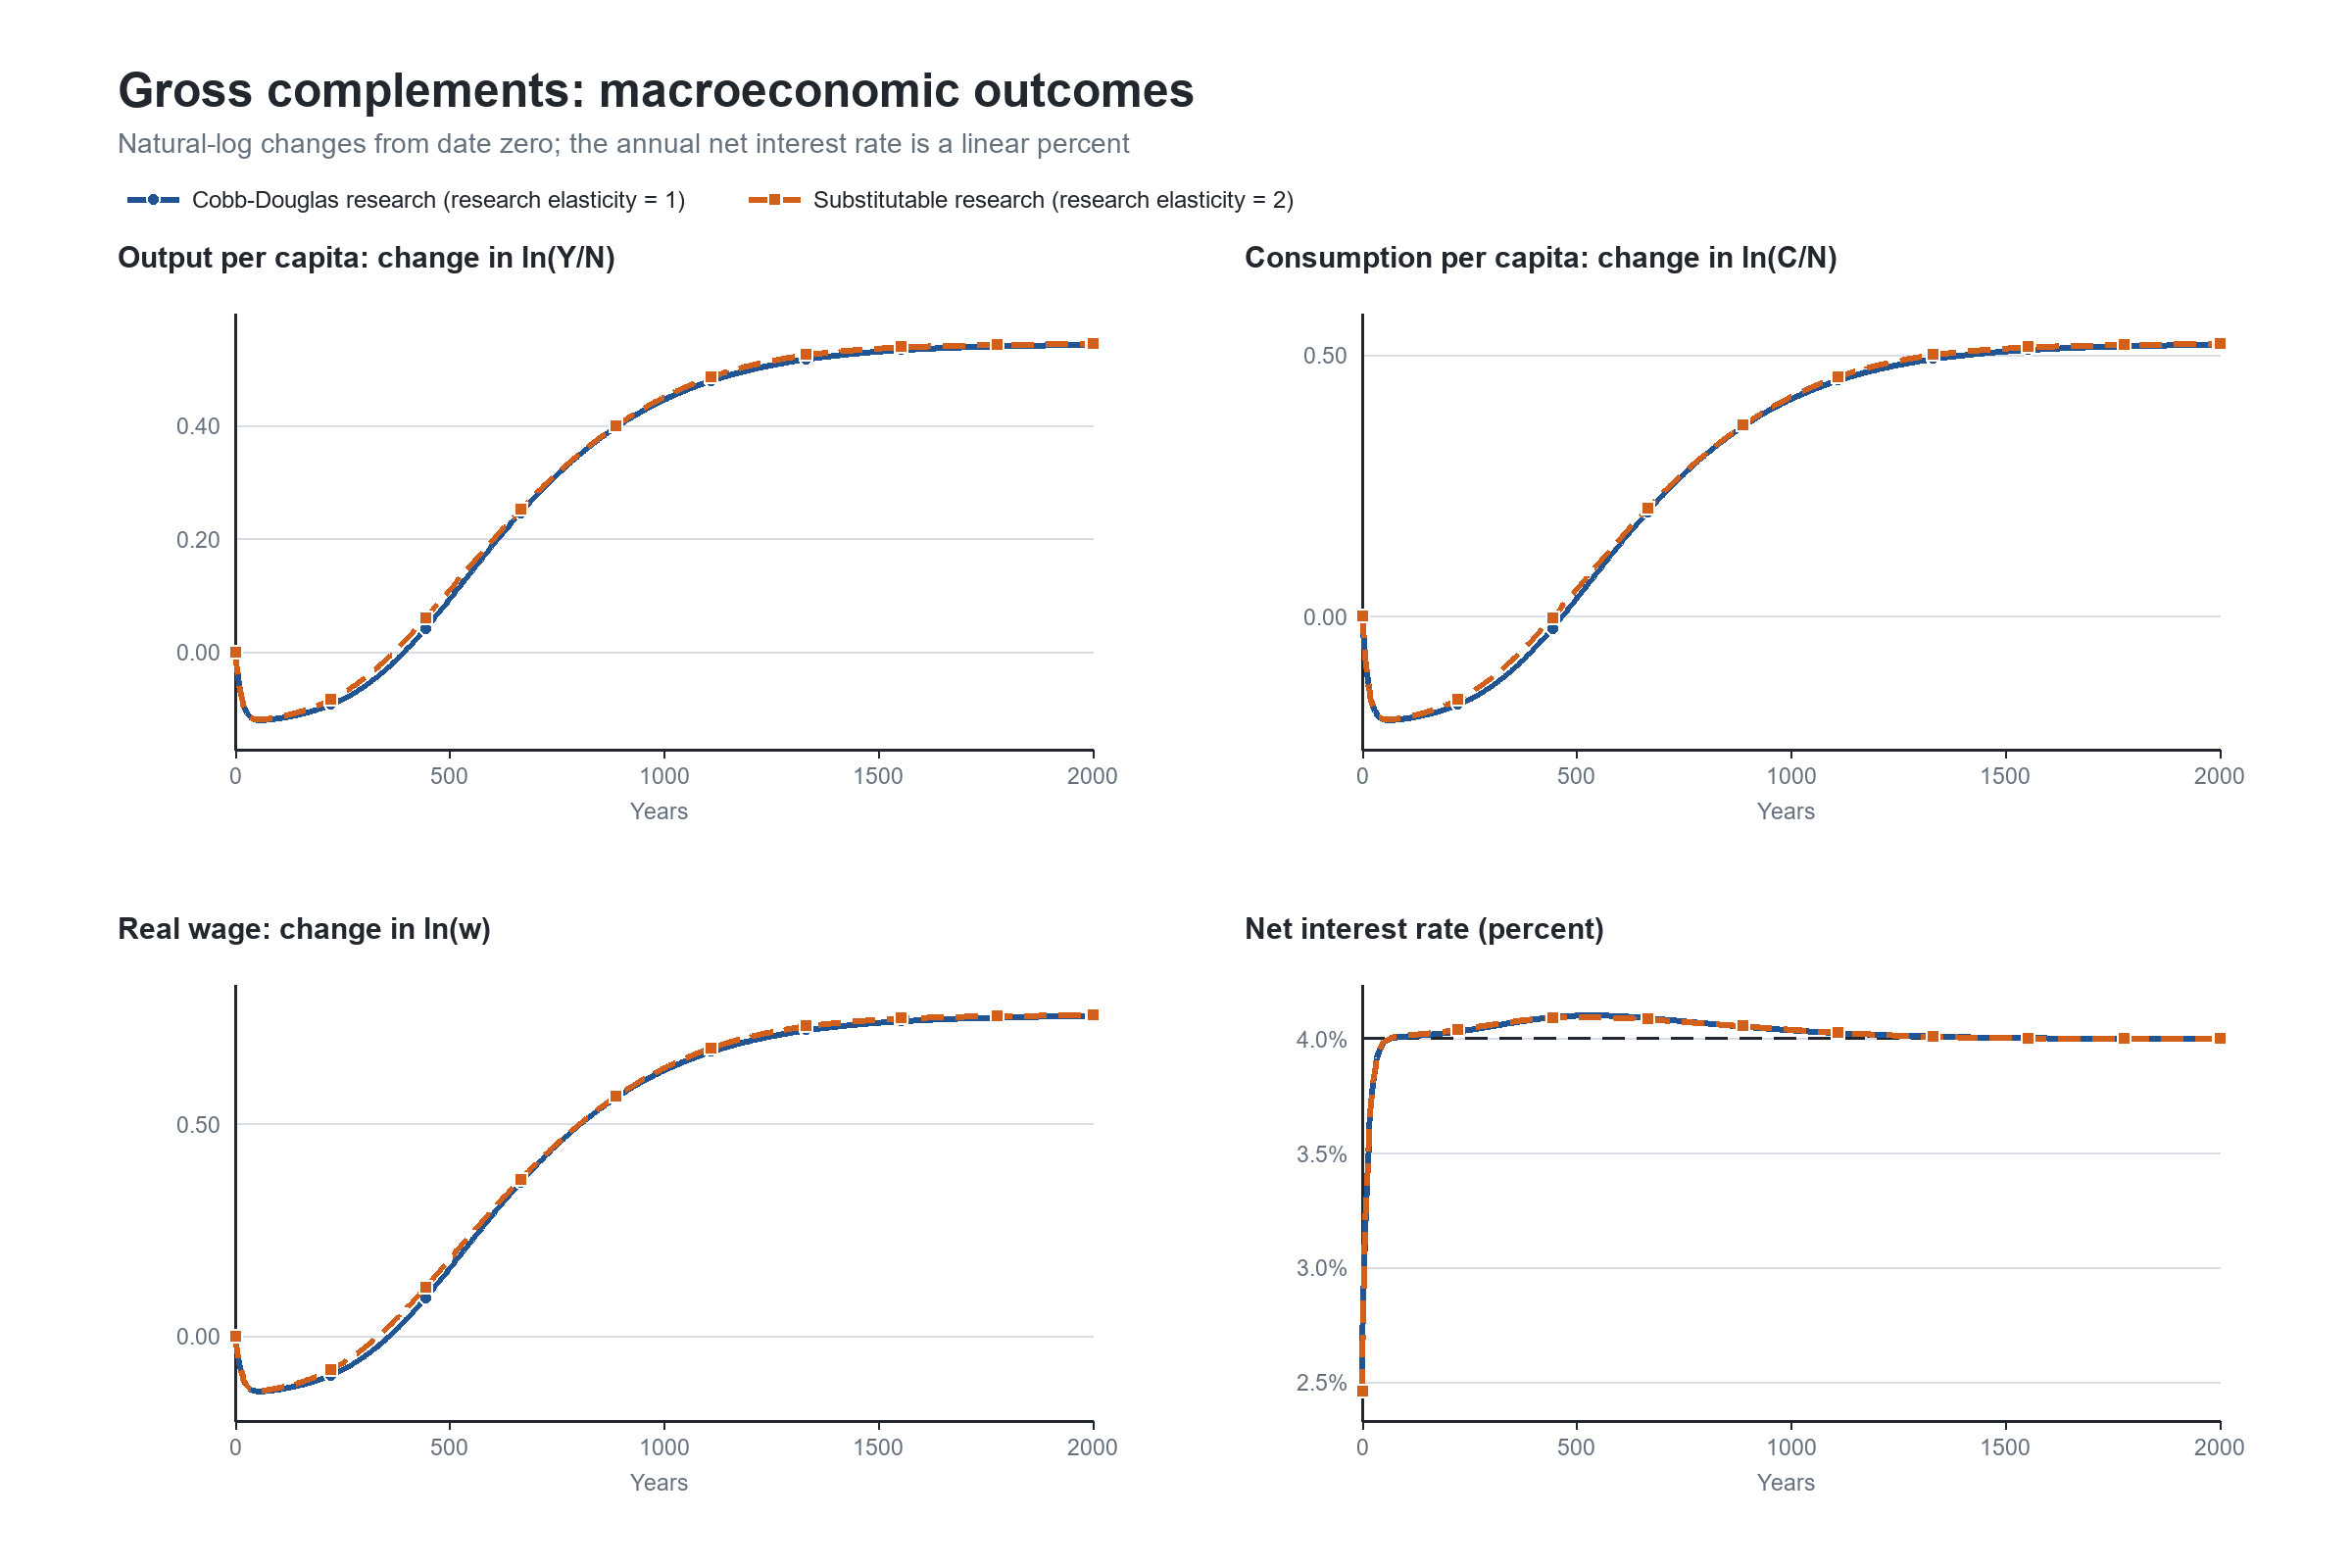
\includegraphics[width=\textwidth]{figures_axm/axm_complements_macro_prices.png}
\caption{Macroeconomic transition with \(\sigma_{XL}=0.75\). The first three
panels show natural-log changes from date zero; the last shows the annual net
interest rate. Blue solid lines use \(\sigma_{HM}=1\), and orange dashed lines
use \(\sigma_{HM}=2\). Model time is a numerical normalization, not a dated
forecast.}
\label{fig:axm-complement-macro}
\end{figure}

Figure \ref{fig:axm-complement-shares} shows the bottleneck directly. Production
labor approaches the population, \(X/(AL)\) approaches a finite ratio, inference
compute vanishes relative to output, and labor retains a positive income share.

\begin{figure}[H]
\centering
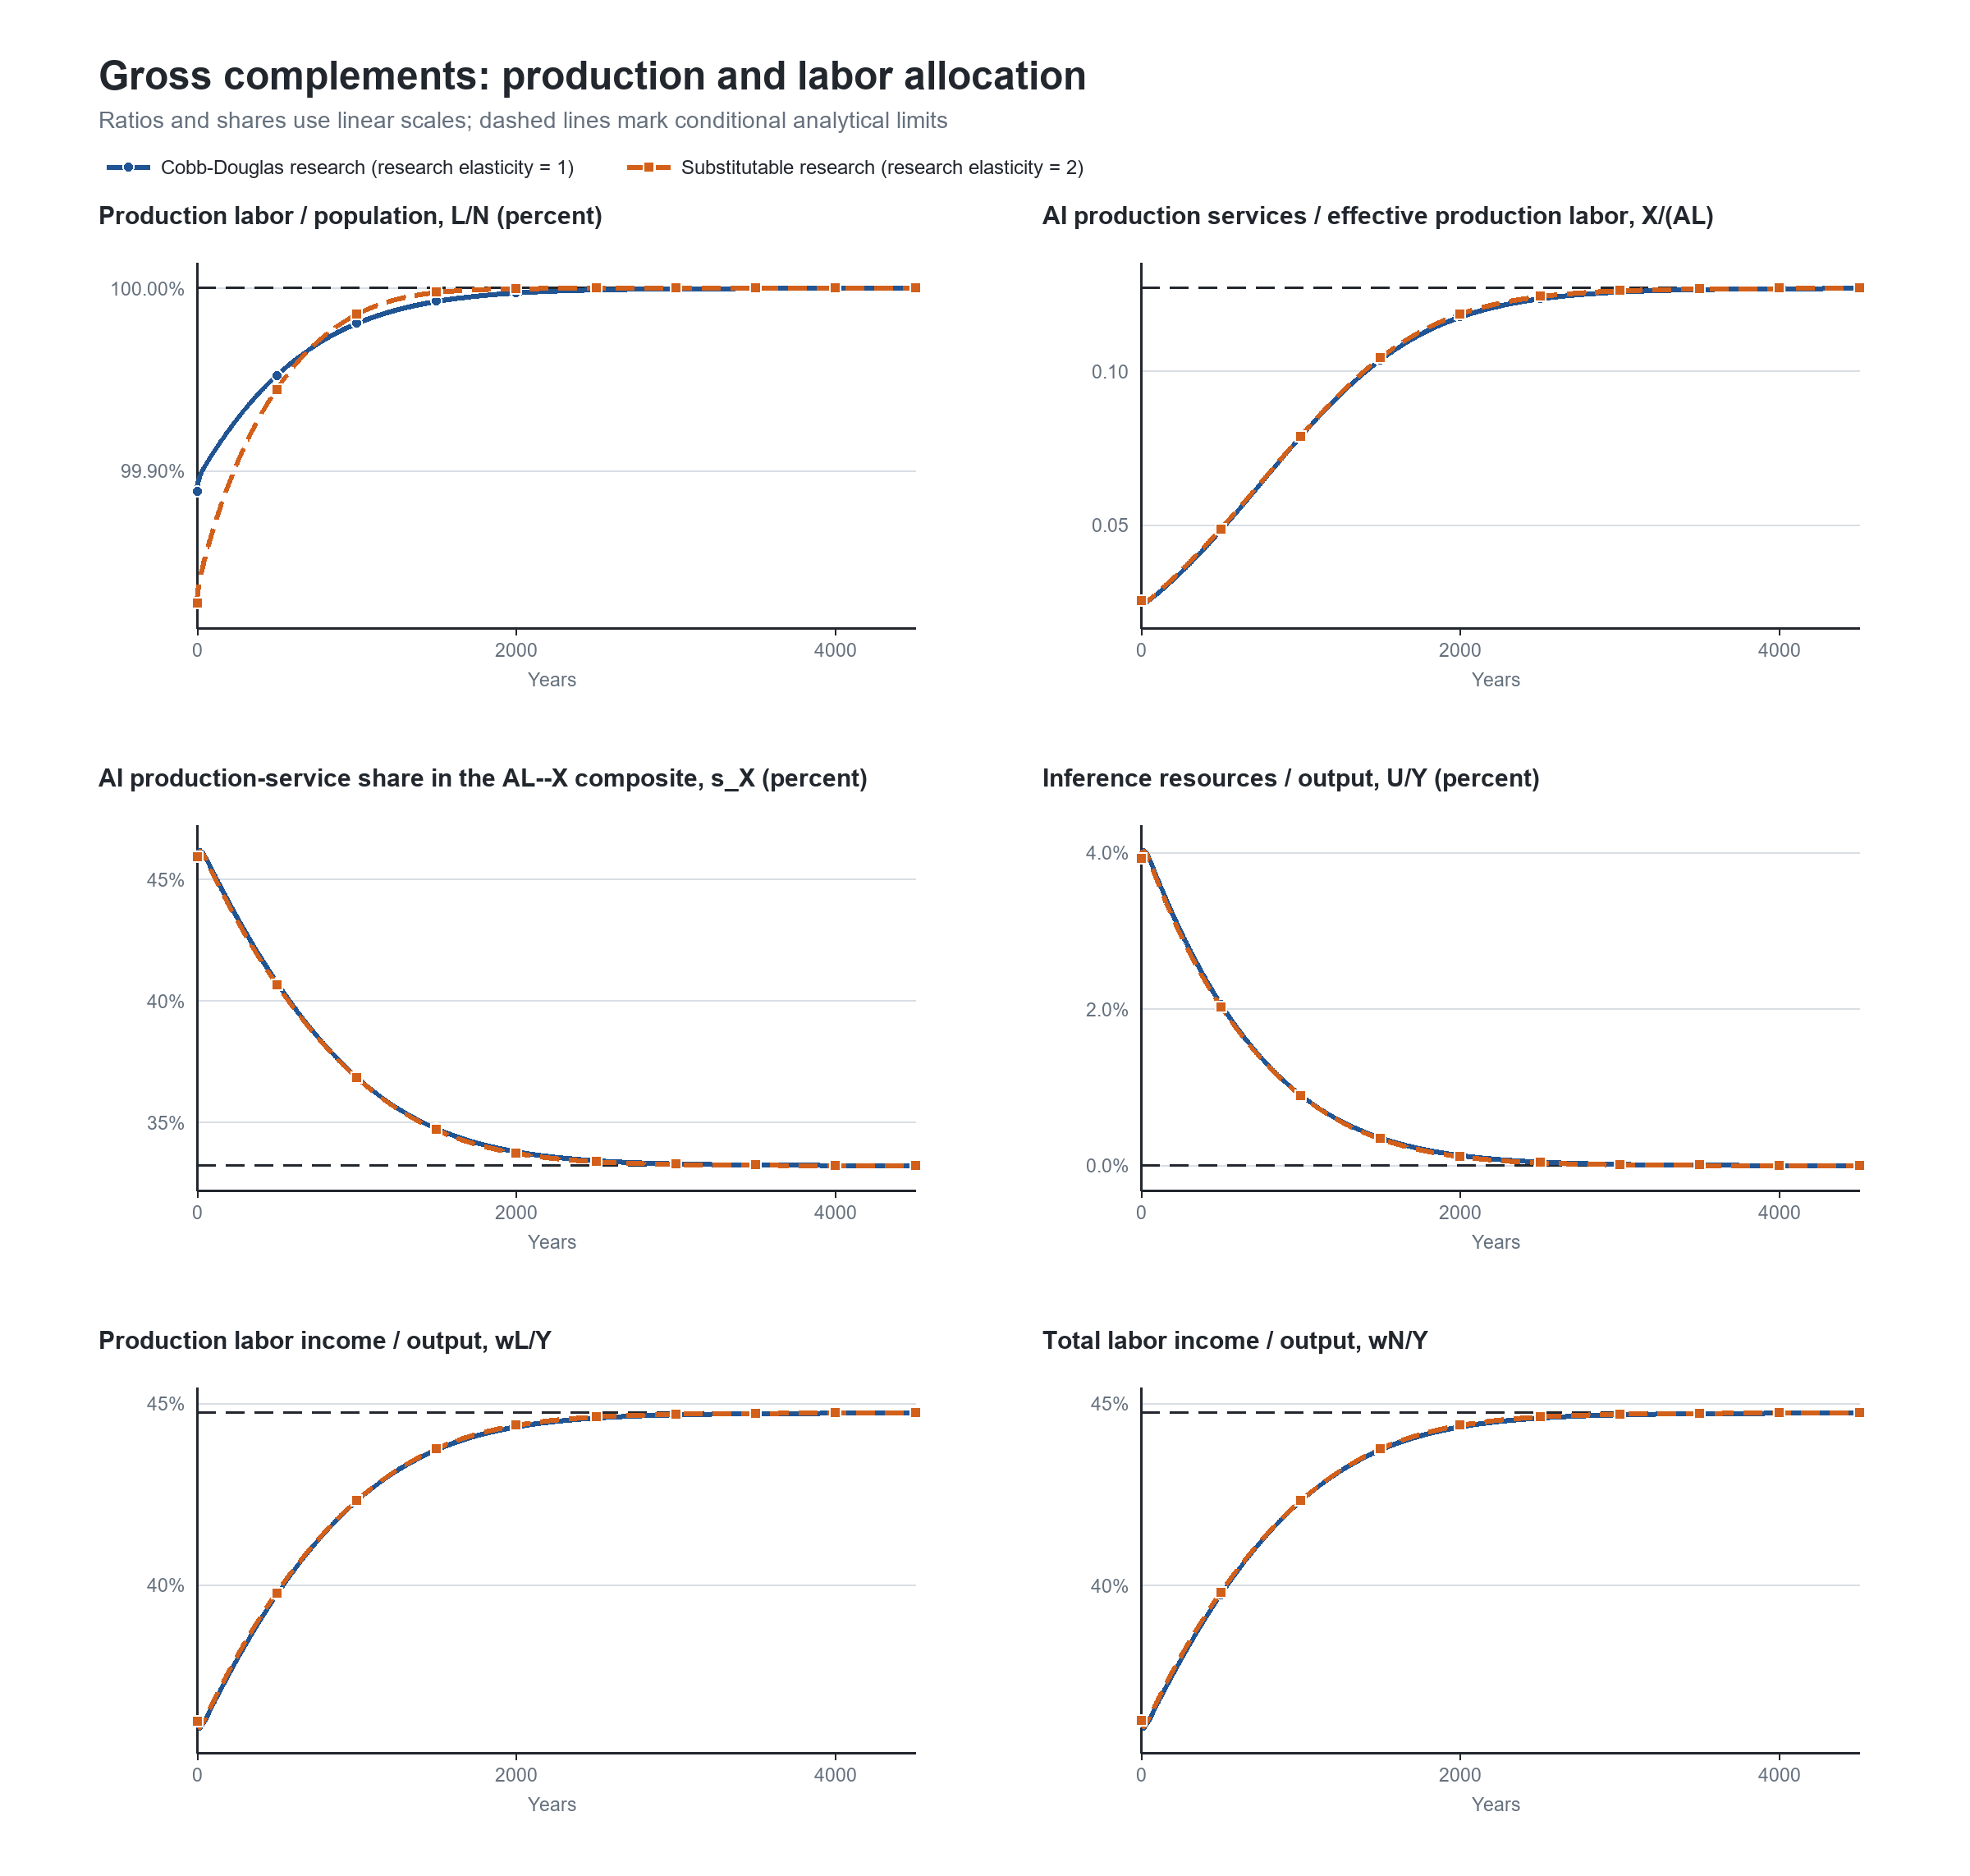
\includegraphics[width=\textwidth]{figures_axm/axm_complements_factor_shares_automation.png}
\caption{Production and labor allocation with \(\sigma_{XL}=0.75\). Here
\(s_X\) is AI production services' technological share within the labor--AI composite, not
their final-output income share. Ratios and shares use linear scales; the
\(L/N\) panel uses a focused vertical scale. Horizontal reference lines are
conditional analytical limits.}
\label{fig:axm-complement-shares}
\end{figure}

Figure \ref{fig:axm-complement-research} shows that research can still become
almost fully automated. With substitutable research inputs, \(s_M\) approaches
one and \(H/N\) approaches zero, while capability continues to rise.

\begin{figure}[H]
\centering
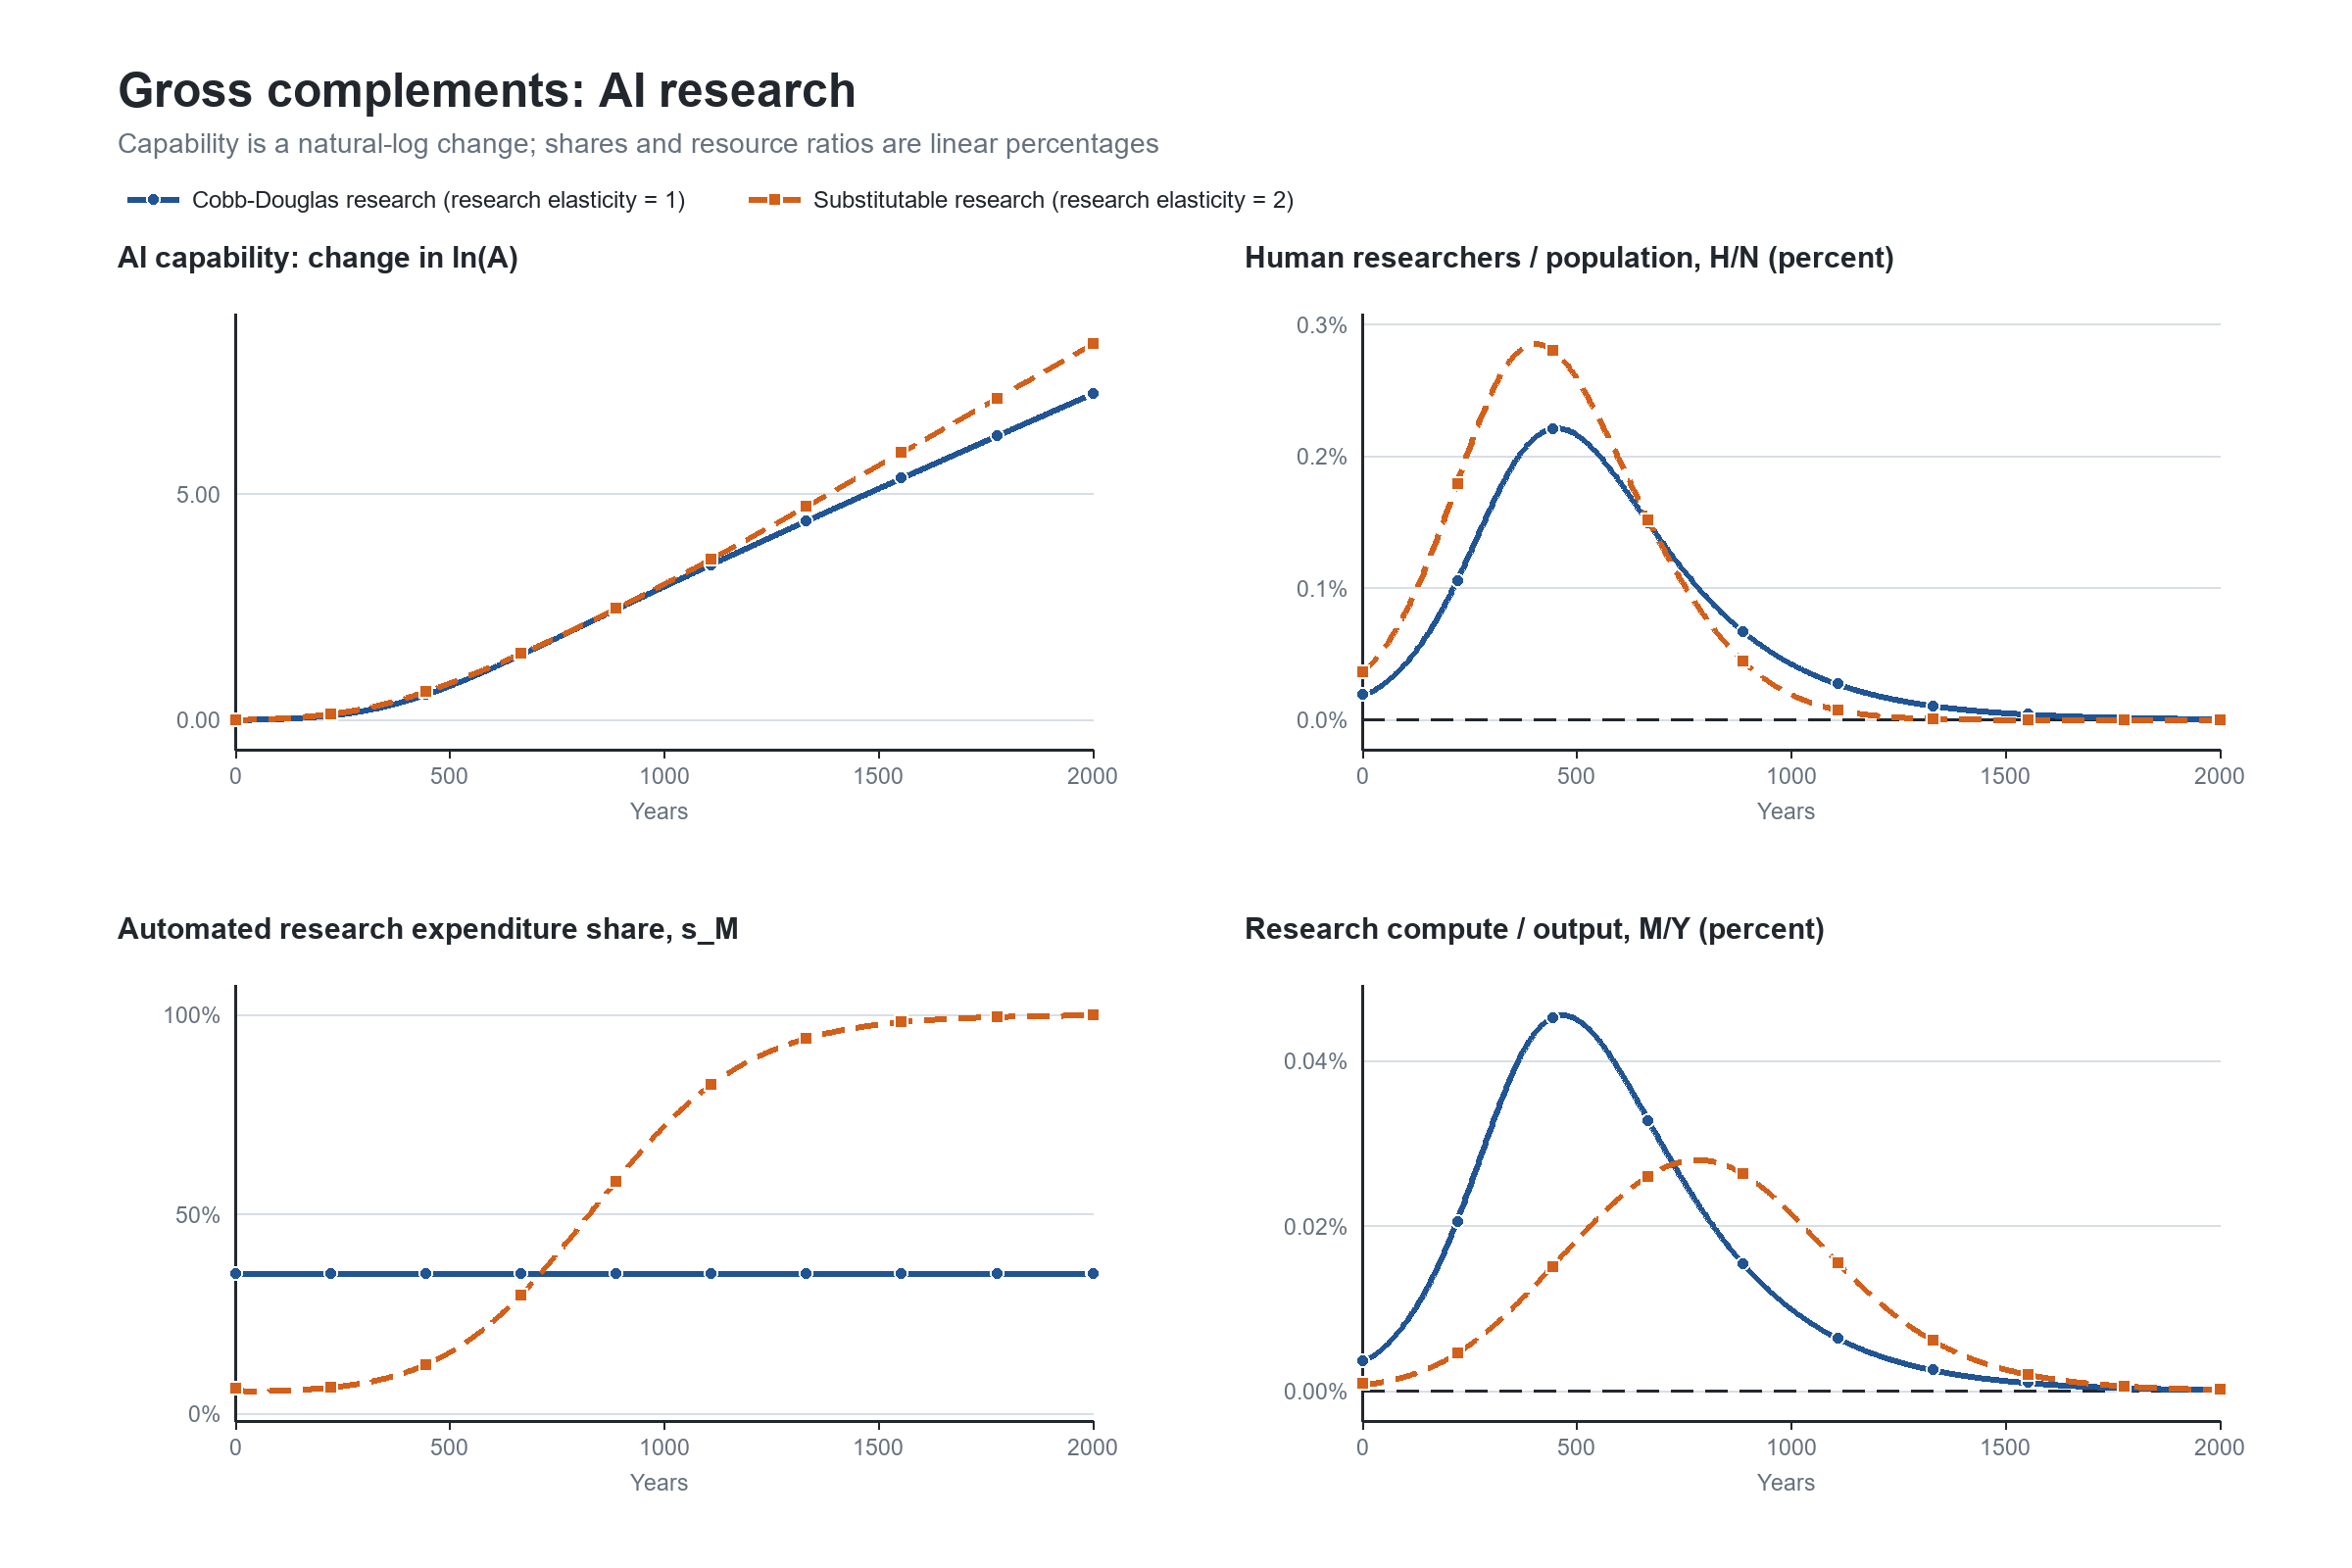
\includegraphics[width=\textwidth]{figures_axm/axm_complements_research_resources.png}
\caption{AI research with \(\sigma_{XL}=0.75\). Capability is shown as a
natural-log change from date zero. The human-research population share, the
share of research expenditure allocated to AI research services, and research compute relative to output
are percentages on linear scales. Positive allocations at every saved finite
date preserve interiority even as \(H/N\) and \(M/Y\) approach zero.}
\label{fig:axm-complement-research}
\end{figure}

At the terminal date with substitutable research, \(s_M=0.99982\) and
\(H/N=1.8\times10^{-11}\), yet labor's aggregate income share approaches 0.4474.
Research automation therefore does not remove the production bottleneck.

\subsection{Cases II and III: unit elasticity in final production}

The two unit-elasticity cases share the same final-production reduction. They
differ in the research-input limit and are therefore presented with a common
analytical characterization followed by separate case implications and a joint
numerical comparison.

\subsubsection{Common analytical characterization}

Set \(\sigma_{XL}=1\), and define
\begin{equation}
 \beta=(1-\alpha)\omega_X,\qquad
 \lambda=(1-\alpha)\omega_L,\qquad
 \nu=\frac{\beta}{\lambda}=\frac{\omega_X}{\omega_L}.
 \label{eq:axm-cd-definitions}
\end{equation}
Combining the final-good firm's AI-demand condition, the monopolist's markup
condition, and market clearing for AI production services with \(X=BU\) gives
\begin{equation}
 \frac{U}{Y}=\beta^2,
 \label{eq:axm-inference-share-cd}
\end{equation}
Substituting that identity into final production gives the reduced equation
\begin{equation}
 Y^{1-\beta}
 =K^\alpha(AL)^\lambda(\beta^2B)^\beta.
 \label{eq:axm-reduced-cd}
\end{equation}
On a balanced path with constant \(K/Y\) and a positive constant \(L/N\), this
equation gives
\begin{equation}
 g_Y=n+\gamma_A+\nu g_B.
 \label{eq:axm-output-growth-cd}
\end{equation}

It is useful to treat Cobb--Douglas research and research that asymptotically relies on AI research services
separately. Let
\begin{equation}
 \bar s=
 \begin{cases}
  \omega_M,&\sigma_{HM}=1,\\
  1,&\sigma_{HM}>1\text{ and }Bw\to\infty.
 \end{cases}
 \label{eq:axm-sbar}
\end{equation}
Define the feedback denominator
\begin{equation}
 D(\bar s)=1-\eta\bar s(1+\nu).
 \label{eq:axm-feedback-denominator}
\end{equation}

\begin{proposition}[Balanced-growth candidates at unit elasticity]
\label{prop:axm-cd-bgp}
Suppose \(\sigma_{XL}=1\), research remains interior, total research expenditure
\((wH+M)/Y\) converges to a positive output share, and \(K/Y\), \(C/Y\), and
\(L/N\) converge to positive constants. Suppose also that \(g_B\) converges to a
positive constant regularly, in the sense that \(\dot g_B/g_B\to0\).

\begin{enumerate}[label=(\roman*)]
\item If \(\sigma_{HM}=1\), every such balanced-growth equilibrium must have
 \(D(\omega_M)>0\).
\item If \(\sigma_{HM}>1\), the balanced-growth restrictions imply
 \(Bw\to\infty\) and \(s_M\to1\); every such equilibrium must have \(D(1)>0\).
\end{enumerate}

If the relevant denominator is positive, the only growth rates consistent with
these necessary restrictions are
\begin{equation}
 g_B=\frac{\eta(n+\bar s\gamma_A)}{D(\bar s)},\qquad
 g_Y=g_K=g_C=n+\gamma_A+\nu g_B,\qquad
 g_w=\gamma_A+\nu g_B.
 \label{eq:axm-cd-growth-rates}
\end{equation}
The remaining prices and quantities have the candidate rates
\begin{align}
 g_U&=g_M=g_Y,&
 g_X&=g_Y+g_B,&
 g_{p_X}&=-g_B,\\
 g_q&=g_Y-g_B,&
 g_E&=\frac{g_B}{\eta},&
 g_L&=n.
 \label{eq:axm-cd-remaining-rates}
\end{align}
Human research satisfies
\begin{equation}
 g_H=
 \begin{cases}
 n,&\sigma_{HM}=1,\\
 n-(\sigma_{HM}-1)[\gamma_A+(1+\nu)g_B],
 &\sigma_{HM}>1,\ s_M\to1.
 \end{cases}
 \label{eq:axm-human-research-growth}
\end{equation}
Thus \(H/N\) converges to a positive constant in the Cobb--Douglas research
case, whereas it falls asymptotically at rate
\((\sigma_{HM}-1)[\gamma_A+(1+\nu)g_B]\) when research inputs are gross substitutes.
Let \(\gamma=\gamma_A+\nu g_B\). The candidate output shares are
\begin{align}
 u&\equiv\frac{U}{Y}=\beta^2,\\
 i&\equiv\frac{\dot K+\delta K}{Y}
 =\frac{\alpha(n+\gamma+\delta)}{\rho+\delta+\gamma},\\
 m&\equiv\frac{M}{Y}
 =\frac{\beta^2\eta\bar s\,g_B}
 {\rho-n+(1-\eta\bar s)g_B},\\
 c&\equiv\frac{C}{Y}=1-u-i-m.
 \label{eq:axm-cd-shares}
\end{align}
The denominator in \(m\) is positive under \(\rho>n\), \(0<\eta<1\), and
\(0<\bar s\leq1\).
The computed share \(c\) must coincide with the positive limit hypothesized above.
An interior equilibrium also requires the monopoly second-order condition and
nonnegative limiting values of \(L/N\) and \(H/N\) that sum to one. Under the
maintained restriction \(\rho>n\), the candidate also satisfies both
transversality conditions.
\end{proposition}

The proposition states necessary growth restrictions and lists the remaining
conditions needed for existence; it does not infer existence from \(D>0\) alone.

The Cobb--Douglas research case admits a stronger constructive result. Define
\begin{equation}
 \ell^*=\frac{\lambda\omega_M}
 {\lambda\omega_M+m^*\omega_H},
 \label{eq:axm-cd-human-labor-share}
\end{equation}
where \(m^*\) is the share in \eqref{eq:axm-cd-shares} evaluated at
\(\bar s=\omega_M\).

\begin{proposition}[Existence and local selection with Cobb--Douglas human research]
\label{prop:axm-cd-human-existence}
Suppose \(\sigma_{XL}=\sigma_{HM}=1\), \(D(\omega_M)>0\),
\(\beta\leq1/2\), \(\eta(1+\omega_M)\leq1\), \(\rho>n\), and the
shares in \eqref{eq:axm-cd-shares} satisfy \(c^*>0\). Then, for every
\(A_0,N_0>0\), there are positive \(K_0,B_0,C_0,q_0\) and a regular interior
balanced-growth equilibrium with \(L/N=\ell^*\).

At the baseline calibration \(\gamma_A=0\), the normalized Jacobian has roots
\begin{equation}
 -0.08967,\qquad -0.002945,\qquad 0.03100,\qquad 0.12971.
 \label{eq:axm-cd-human-jacobian-roots}
\end{equation}
The projection of its stable eigenspace onto \((K,B)\) is nonsingular.
Consequently, consumption and the shadow value of capability are locally unique
functions of the two predetermined stocks, and the resulting nearby paths
converge to the balanced-growth equilibrium.
\end{proposition}

The result does not apply the automated benchmark's Jacobian to a model with
human research. The Appendix derives the human-research Jacobian from its own
labor-allocation and research equations. When \(\sigma_{HM}>1\), human research
vanishes only asymptotically; the corresponding finite-date Jacobian must be
computed from the interior static map.

\paragraph{Feedback-matrix interpretation.}
The feedback accounting of \citet{davidsonetal2026} makes the denominator
transparent. Let \(\widetilde g_Y=g_Y-(n+\gamma_A)\). The limiting balanced-growth
restrictions can be written as
\begin{equation}
 \begin{pmatrix}g_B\\ \widetilde g_Y\end{pmatrix}
 =
 \begin{pmatrix}\eta(n+\bar s\gamma_A)\\0\end{pmatrix}
 +
 \underbrace{\begin{pmatrix}
  \eta\bar s&\eta\bar s\\
  \nu&0
 \end{pmatrix}}_{\mathcal F(\bar s)}
 \begin{pmatrix}g_B\\ \widetilde g_Y\end{pmatrix}.
 \label{eq:axm-feedback-matrix}
\end{equation}
The upper-left entry is the technological loop
\(B\to BM\to\dot B\). The off-diagonal cycle is the economic loop
\(B\to Y\to M\to BM\to\dot B\). Consequently,
\begin{equation}
 \det[I-\mathcal F(\bar s)]
 =1-\eta\bar s(1+\nu)=D(\bar s),
 \qquad
 r_{\mathrm{sp}}(\mathcal F)
 =\frac{\eta\bar s+
 \sqrt{(\eta\bar s)^2+4\eta\bar s\nu}}{2}.
 \label{eq:axm-feedback-radius}
\end{equation}
Here \(r_{\mathrm{sp}}\) denotes the spectral radius; this notation avoids
confusing it with the household discount rate \(\rho\). Because \(\mathcal F\)
is nonnegative, \(r_{\mathrm{sp}}(\mathcal F)<1\) if and only if
\(D(\bar s)>0\). In that case,
\[
 \begin{pmatrix}g_B\\ \widetilde g_Y\end{pmatrix}
 =[I-\mathcal F(\bar s)]^{-1}
 \begin{pmatrix}\eta(n+\bar s\gamma_A)\\0\end{pmatrix}.
\]
Thus \(1/D(\bar s)\) is the scalar feedback multiplier after eliminating
\(\widetilde g_Y\), analogous to the relevant element of Davidson et al.'s
Leontief inverse.

Exogenous labor-productivity growth changes the source vector through
\(n+\bar s\gamma_A\), but it does not change the feedback matrix or its
stability threshold.

Equivalently, the reduced technological and economic gains are
\[
 G_T=\eta\bar s,\qquad
 G_E=\eta\bar s\nu,\qquad
 D=1-G_T-G_E.
\]
Table \ref{tab:axm-feedback-accounting} applies this decomposition to the two
unit-elasticity benchmarks. Research substitution raises the total gain from
0.0875 to 0.2500 and the feedback multiplier from 1.096 to 1.333. Even
\(\bar s=1\) remains below the critical value:
\(\bar s_{\mathrm{crit}}=[\eta(1+\nu)]^{-1}=4>1\).

\begin{table}[H]
\centering
\small
\begin{tabular}{lrrrrrr}
\toprule
Research limit & \(\bar s\) & \(G_T\) & \(G_E\) & \(G_T+G_E\) & \(D\) & \(1/D\)\\
\midrule
\(\sigma_{HM}=1\) & 0.35 & 0.0700 & 0.0175 & 0.0875 & 0.9125 & 1.096\\
\(\sigma_{HM}>1,\ s_M\to1\) & 1.00 & 0.2000 & 0.0500 & 0.2500 & 0.7500 & 1.333\\
\bottomrule
\end{tabular}
\caption{Davidson-style feedback accounting for the unit-elasticity benchmark
\citep{davidsonetal2026}. The reduced scalar gain is \(G_T+G_E\).
These are balanced-growth diagnostics, not calibrated probabilities or task
shares.}
\label{tab:axm-feedback-accounting}
\end{table}

This mapping also marks the boundary of what can be imported. Davidson et al.'s
spectral-radius theorem classifies a positive monomial system; their macroeconomic
application obtains such a system under fixed saving and resource-allocation
shares. Here \(D\leq0\) rules out the finite positive
balanced-growth candidate, but does not by itself prove double-exponential growth
or a finite-time singularity. Such a conclusion must also determine prices,
allocations, the developer's costate, and the transversality conditions.

\subsubsection{Adoption from the no-AI balanced-growth path}
\label{sec:axm-ai-adoption-experiment}

I first compare the automated-research benchmark with its no-AI counterfactual.
Before date zero, the economy is on the Ramsey--Cass--Koopmans balanced-growth
path with \(\omega_X=0\). At date zero, \(\omega_X\) increases to 0.20 and
\(\sigma_{XL}=1\). Physical capital, labor productivity, and population are
predetermined, so \(K_0\), \(A_0\), and \(N_0\) are inherited from the no-AI
path.

The no-AI equilibrium does not determine \(B_0\), because capability does not
affect any allocation when \(\omega_X=0\). I therefore calibrate the capability
available at adoption by requiring
\begin{equation}
 Y(0^+;\omega_X=0.20)=Y(0^-;\omega_X=0).
 \label{eq:axm-adoption-output-continuity}
\end{equation}
At unit elasticity, \eqref{eq:axm-inference-share-cd} and
\eqref{eq:axm-reduced-cd} imply that this condition is equivalent to
\(X_0=A_0L_0\). With \(A_0=N_0=L_0=1\), it gives
\begin{equation}
 B_0=\frac{1}{\beta^2Y_0^{\mathrm{RCK}}}=30.9316.
 \label{eq:axm-adoption-initial-capability}
\end{equation}
This value is an adoption-threshold calibration. It is not an equilibrium
condition and does not follow from continuing the positive-AI model through
\(\omega_X=0\). Given \(K_0\) and \(B_0\), the boundary-value problem selects
the jump variables \(C(0^+)\) and \(q(0^+)\). The matching rule isolates the
change in income shares from a mechanical change in initial output, but it does
not identify \(B_0\) empirically. The timing results below are therefore
conditional on \eqref{eq:axm-adoption-output-continuity}. At unit elasticity,
the production-labor, gross-capital, and inference-compute shares are fixed by
the model and do not depend on this matching rule.

The calibration satisfies the restrictions in Proposition
\ref{prop:axm-benchmark-equilibrium-existence}. In particular,
\(\eta=0.20<\alpha=0.33\), \(\beta=0.134<1/2\), \(2\eta=0.40<1\),
\(\Delta=0.402>0\), and \(\rho=0.04>n=0.003\). Hence the positive-AI model
has the analytical balanced-growth equilibrium characterized there. Its
per-capita output growth rate is \(g_Y^*-n=1.0867\) percent and its net
interest rate is \(r^*=5.0867\) percent. The adoption experiment starts far
from that reference path: \(\xi_B(0)=4.2445\). Moreover, the slow stable root
of the normalized system is \(-0.003194\), whose local half-life is about 217
years. Convergence should therefore not be visible within a short simulation
window.

Figure \ref{fig:axm-ai-adoption-macro} compares the two equilibrium paths.
Output does not jump by construction. Consumption falls by 2.26 percent at
adoption, while the real wage falls by 20 percent. The wage falls because the
production-labor share decreases from \(1-\alpha=0.67\) to
\((1-\alpha)\omega_L=0.536\), even though initial output is unchanged. Output
per person subsequently remains close to the no-AI path: after 250 years it is
0.61 percent higher. The net interest rate rises from 5 percent to 5.0035
percent over the same interval---an increase of only 0.0035 percentage points.
Since \(r=\alpha Y/K-\delta\), output continuity and the inherited capital
stock keep the interest rate at 5 percent at adoption. Output then grows
slightly faster than capital, so \(Y/K\) and the interest rate rise slowly.
Panel D extends the interest-rate path to 3,000 years and shows its convergence
to the analytical value \(r^*=5.0867\) percent. Its longer horizontal axis is a
numerical convergence audit, not a calendar forecast.

\begin{figure}[H]
\centering
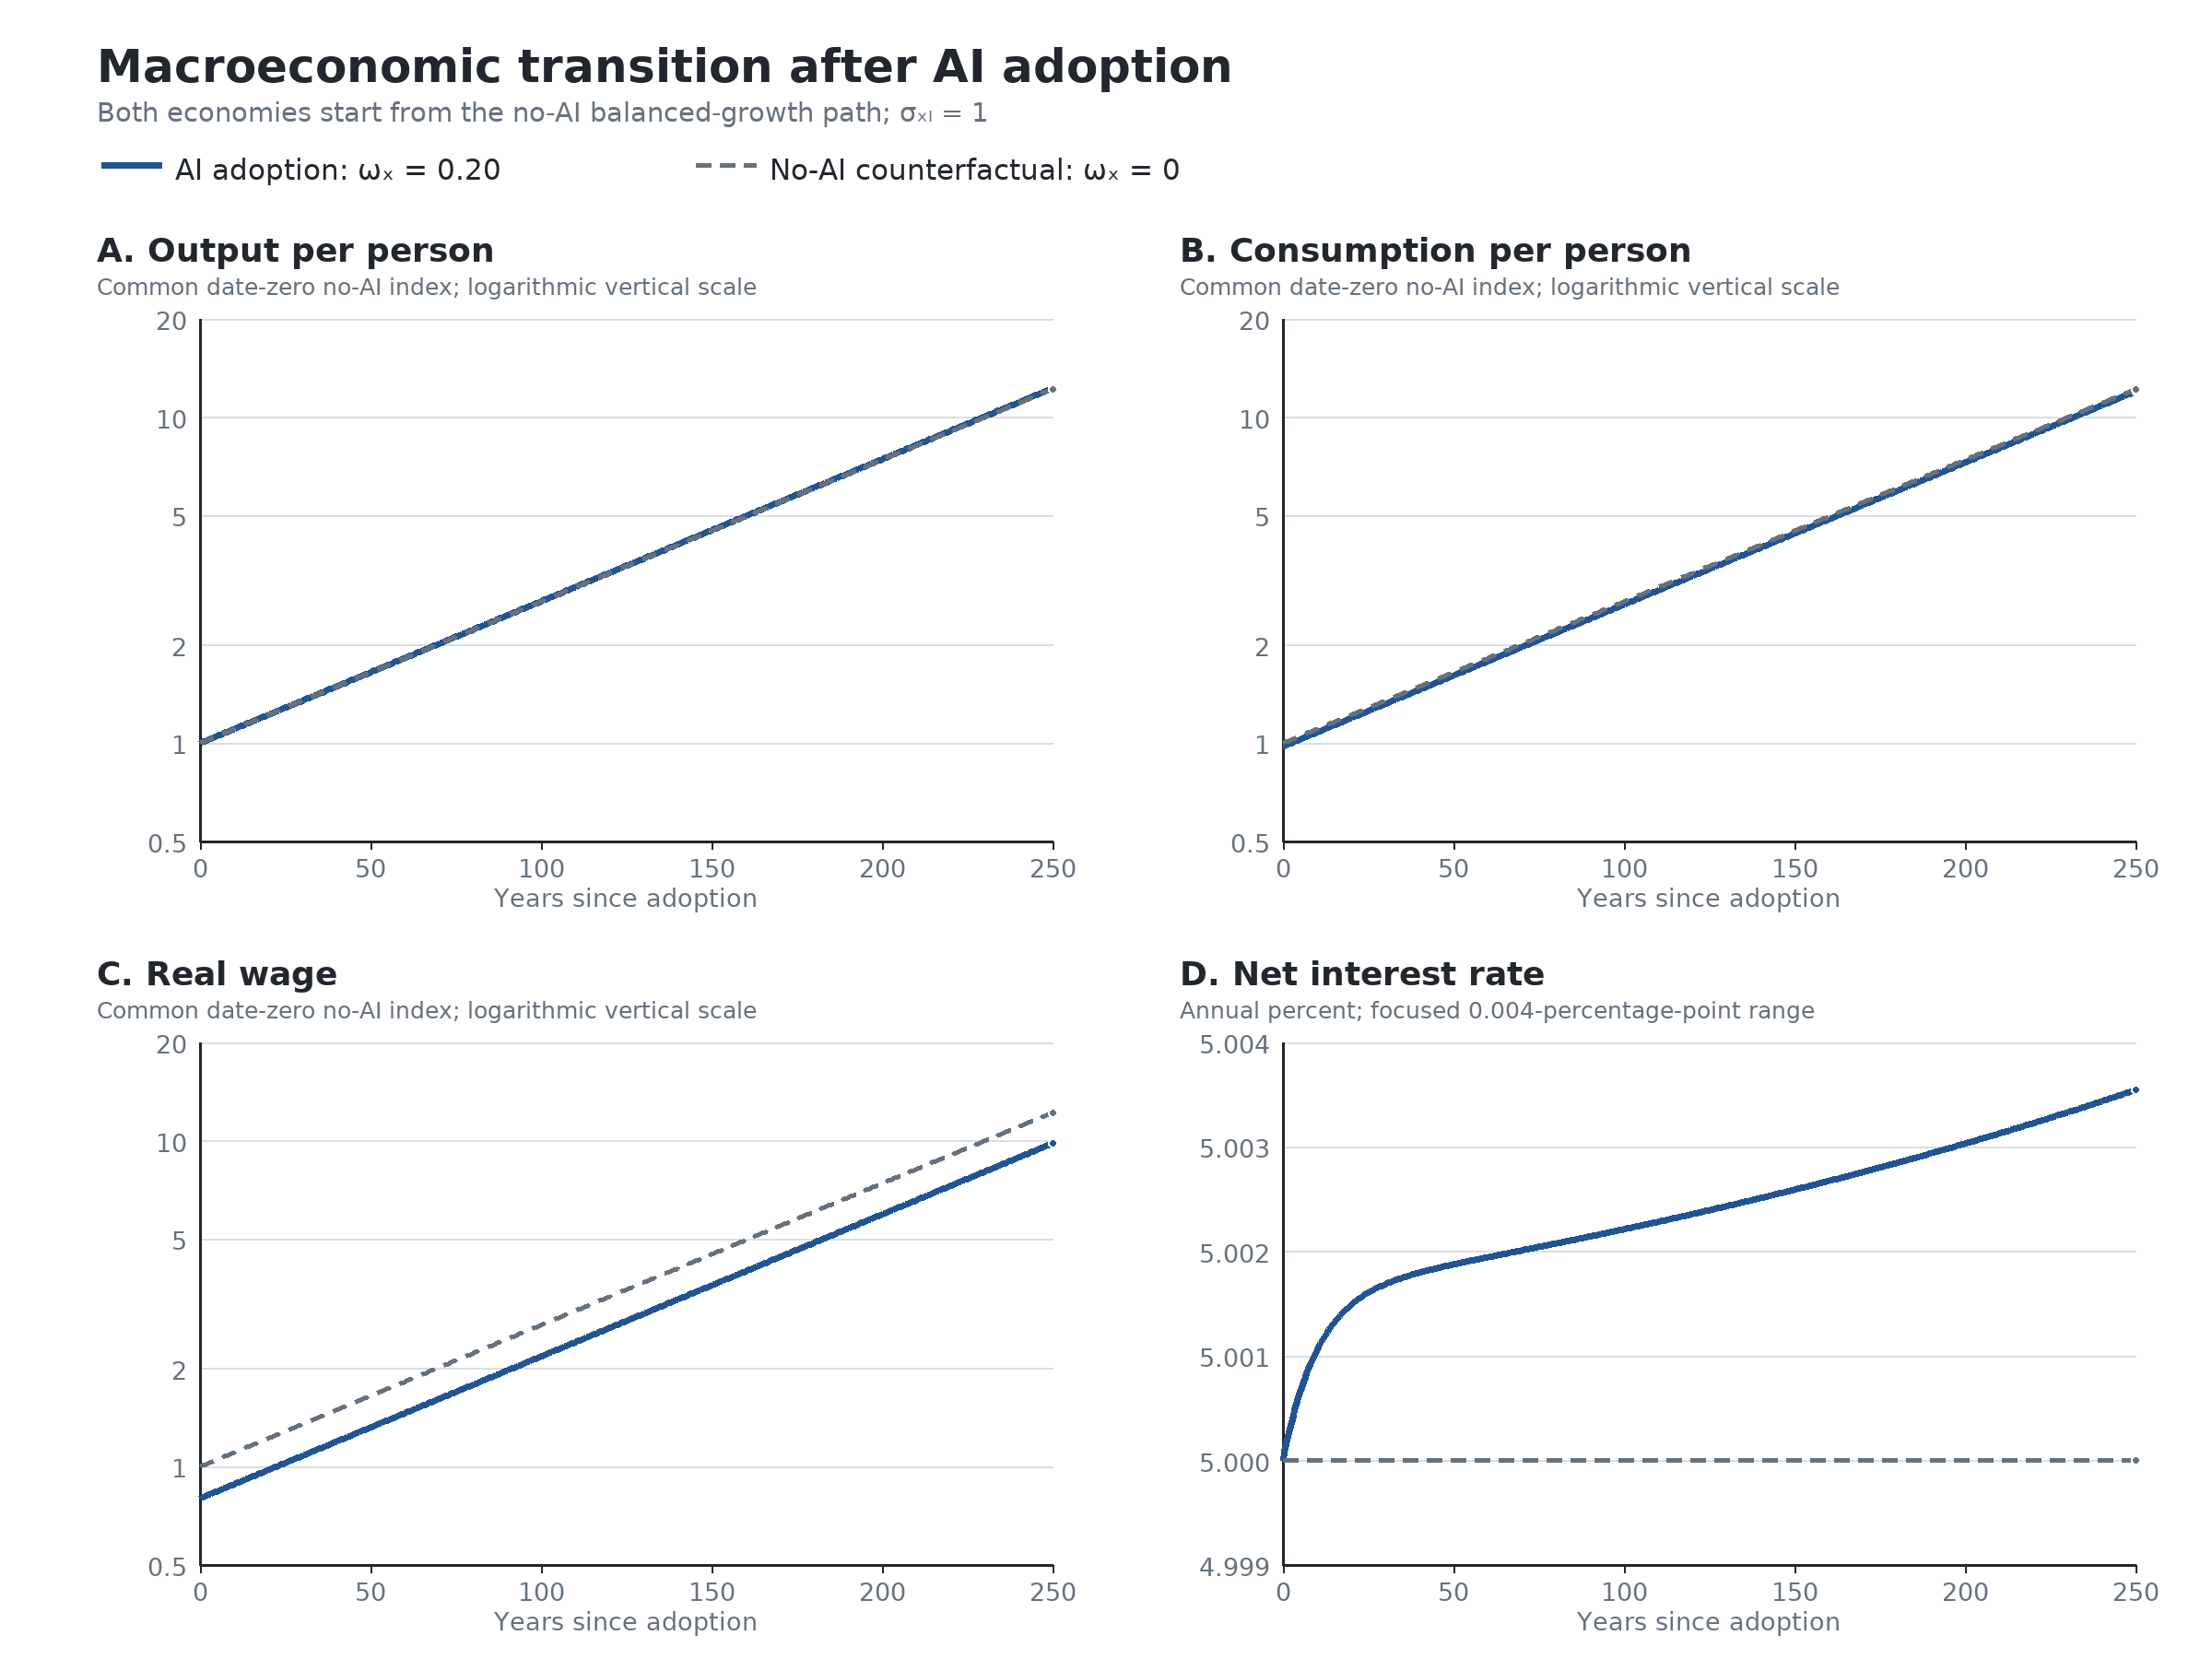
\includegraphics[width=\textwidth]{figures_axm/axm_ai_adoption_macro.png}
\caption{Macroeconomic effects of adopting AI production and autonomous AI
research at date zero. The AI path sets \(\omega_X=0.20\) and
\(\sigma_{XL}=1\); the counterfactual keeps \(\omega_X=0\). Output per person,
consumption per person, and the real wage use a common date-zero no-AI index
and logarithmic vertical scales over the first 250 years. The interest-rate
panel instead displays the full 3,000-year numerical audit; the dotted line is
the analytical balanced-growth value \(r^*=5.0867\) percent. Model time is not
a calendar forecast.}
\label{fig:axm-ai-adoption-macro}
\end{figure}

Figure \ref{fig:axm-ai-adoption-mechanism} explains why the macroeconomic
effects accumulate slowly. The annual growth rate of output per person rises
from 1.0006 percent at adoption to 1.0036 percent after 250 years, and
capability increases by 2.55 percent. The shadow value \(qB/Y\) changes little.
The numerical solution is extended to 3,000 years solely as a convergence
audit. Panel D of Figure \ref{fig:axm-ai-adoption-macro} displays the
interest-rate portion of that audit. At that horizon, per-capita growth is 1.08637 percent and the net
interest rate is 5.08637 percent, both within 0.00030 percentage points of
their analytical balanced-growth values. All other panels show the first 250
years.

\begin{figure}[H]
\centering
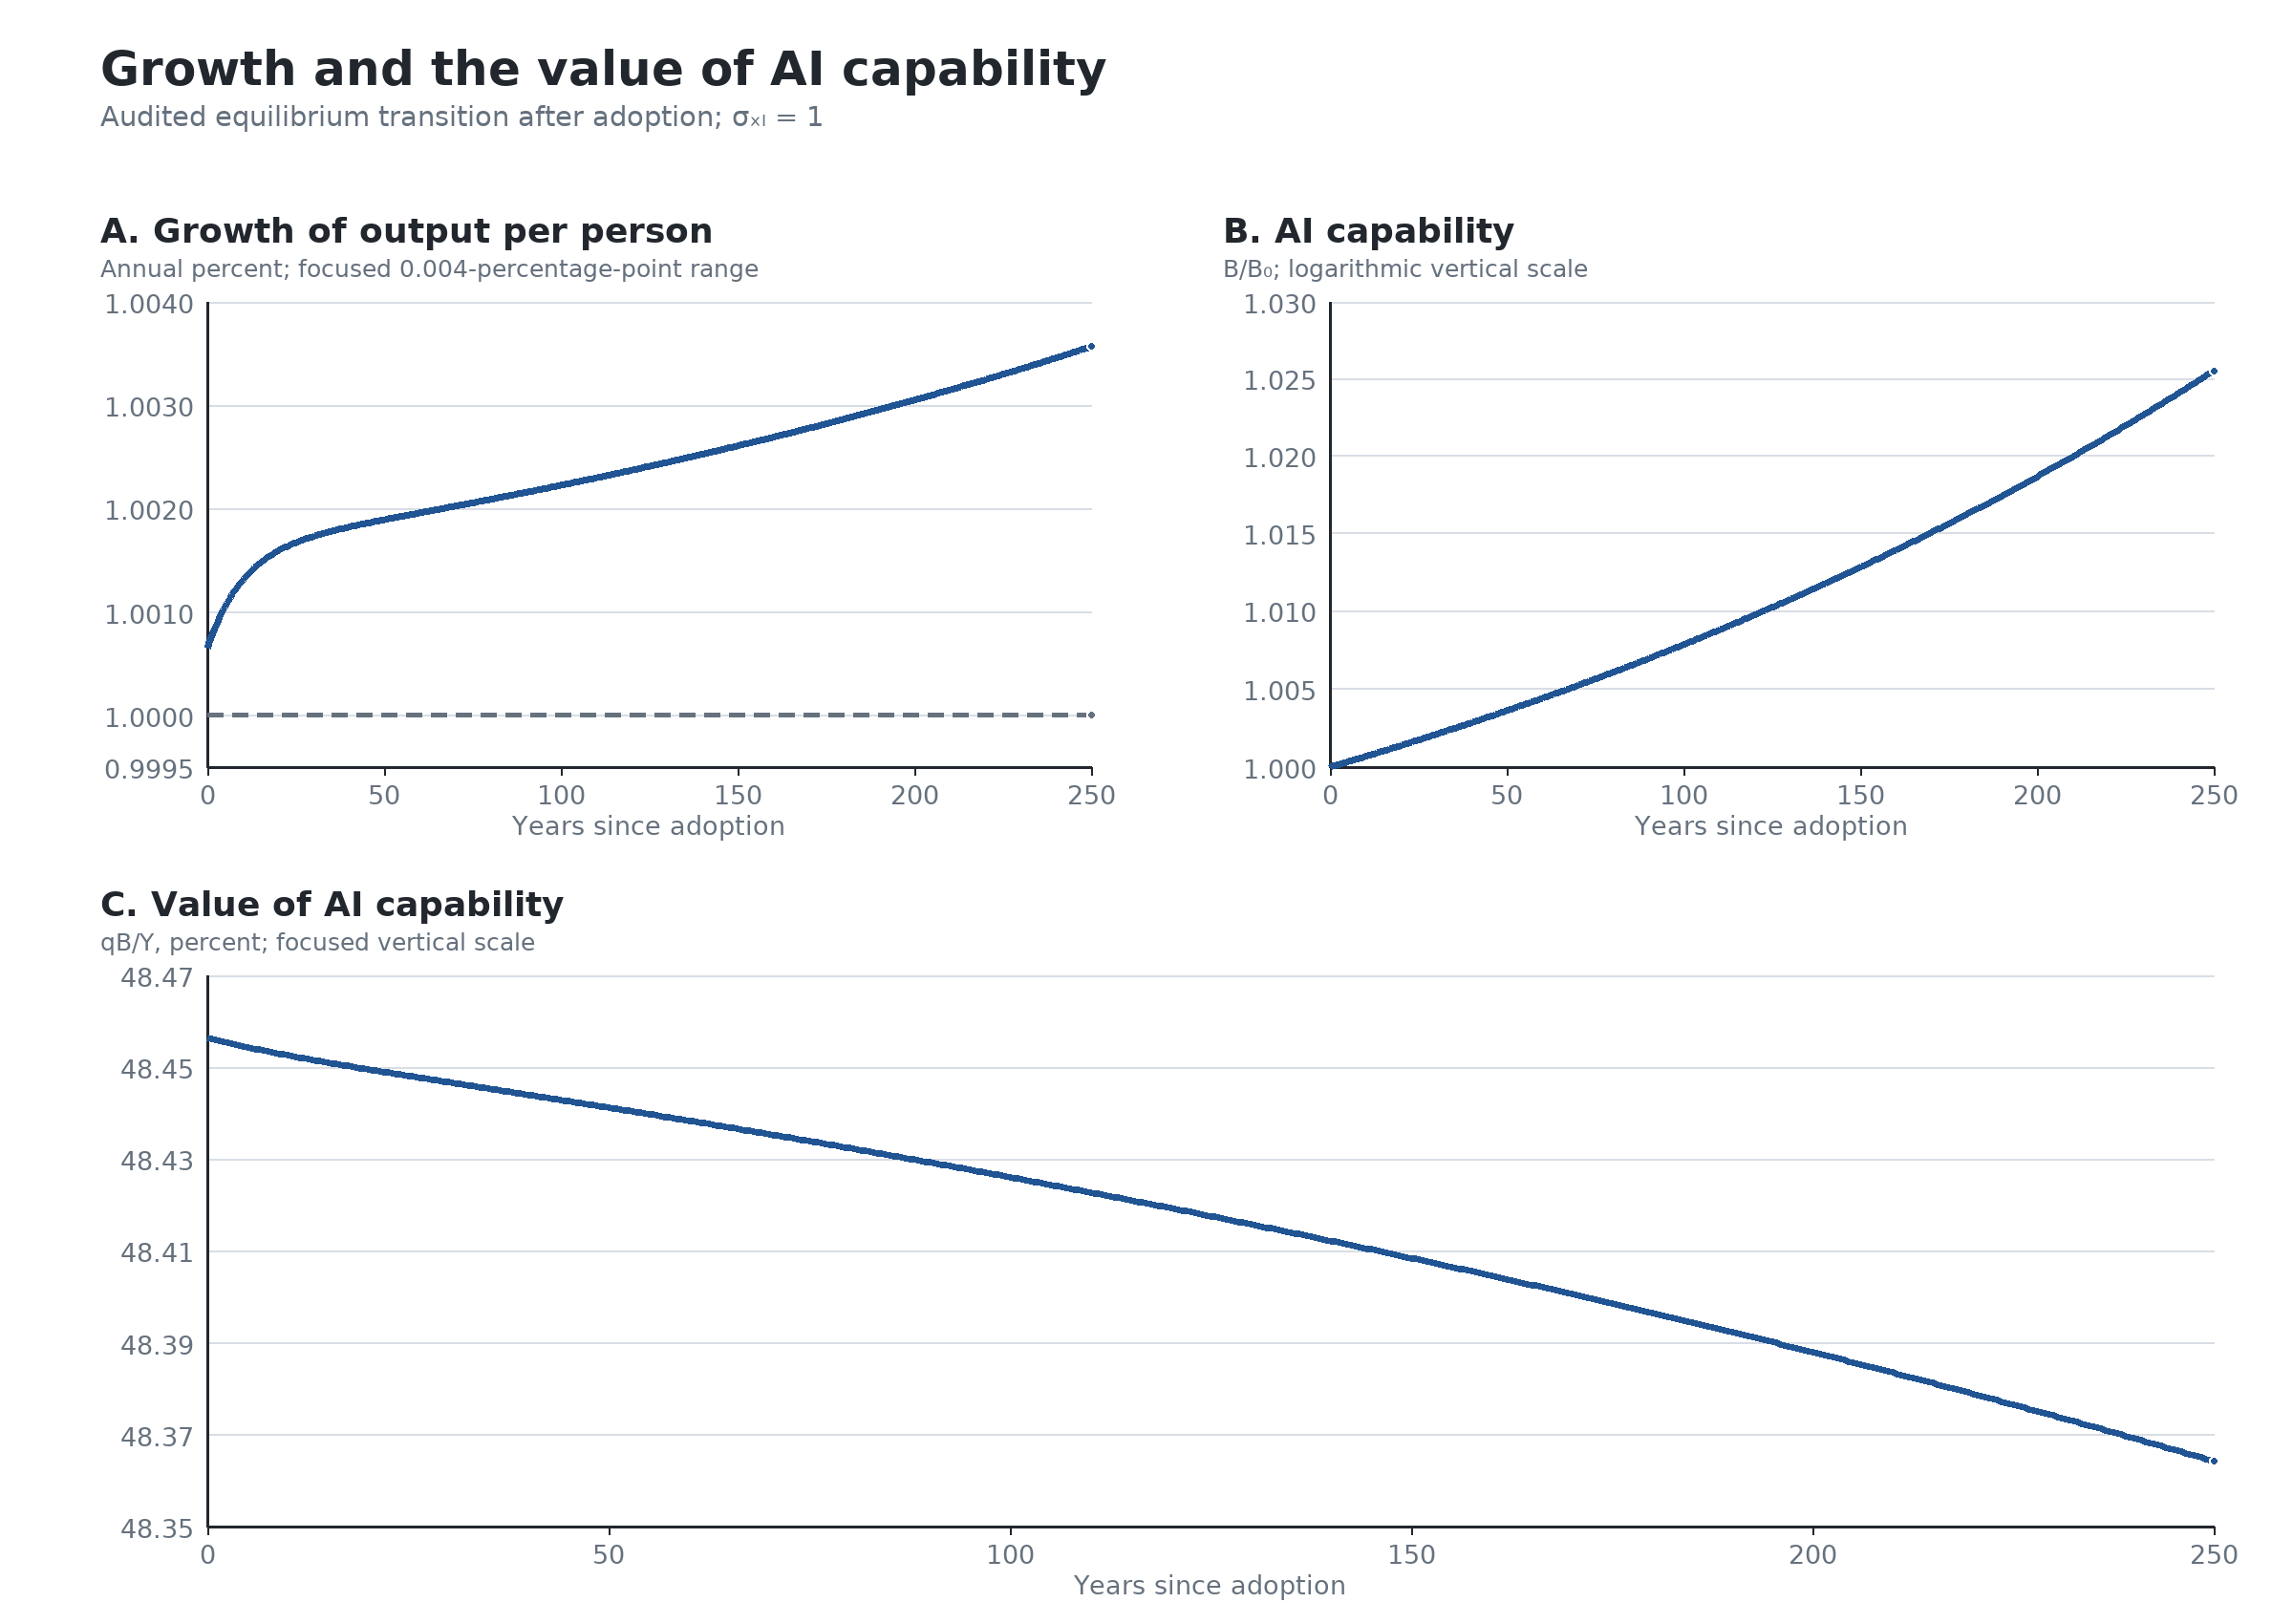
\includegraphics[width=\textwidth]{figures_axm/axm_ai_adoption_mechanism_distribution.png}
\caption{Growth and capability after AI adoption. Growth and \(qB/Y\) use
focused linear scales; the growth panel spans only 0.004 percentage points.
\(B/B_0\) uses a logarithmic scale. The gray dashed line in the first panel is
the no-AI growth rate.}
\label{fig:axm-ai-adoption-mechanism}
\end{figure}

Figure \ref{fig:axm-ai-adoption-distribution-paths} reports the five dated
components of the consolidated output decomposition. The distributional effect
is much larger than the growth effect and occurs immediately. At adoption,
labor's share falls from 67 percent in the no-AI counterfactual to 53.6 percent,
while the gross physical-capital share remains at 33 percent. Along the AI
path, \(wL/Y\), \((r+\delta)K/Y\), and \(U/Y\) remain constant. Over the first
250 years, \(M/Y\) rises from 0.00064 percent to 0.00141 percent of output, and
\(\Pi/Y\) falls by the same 0.00077 percentage points. Thus the large
redistribution occurs when AI enters production; the subsequent transition in
these shares is very small.

\begin{figure}[H]
\centering
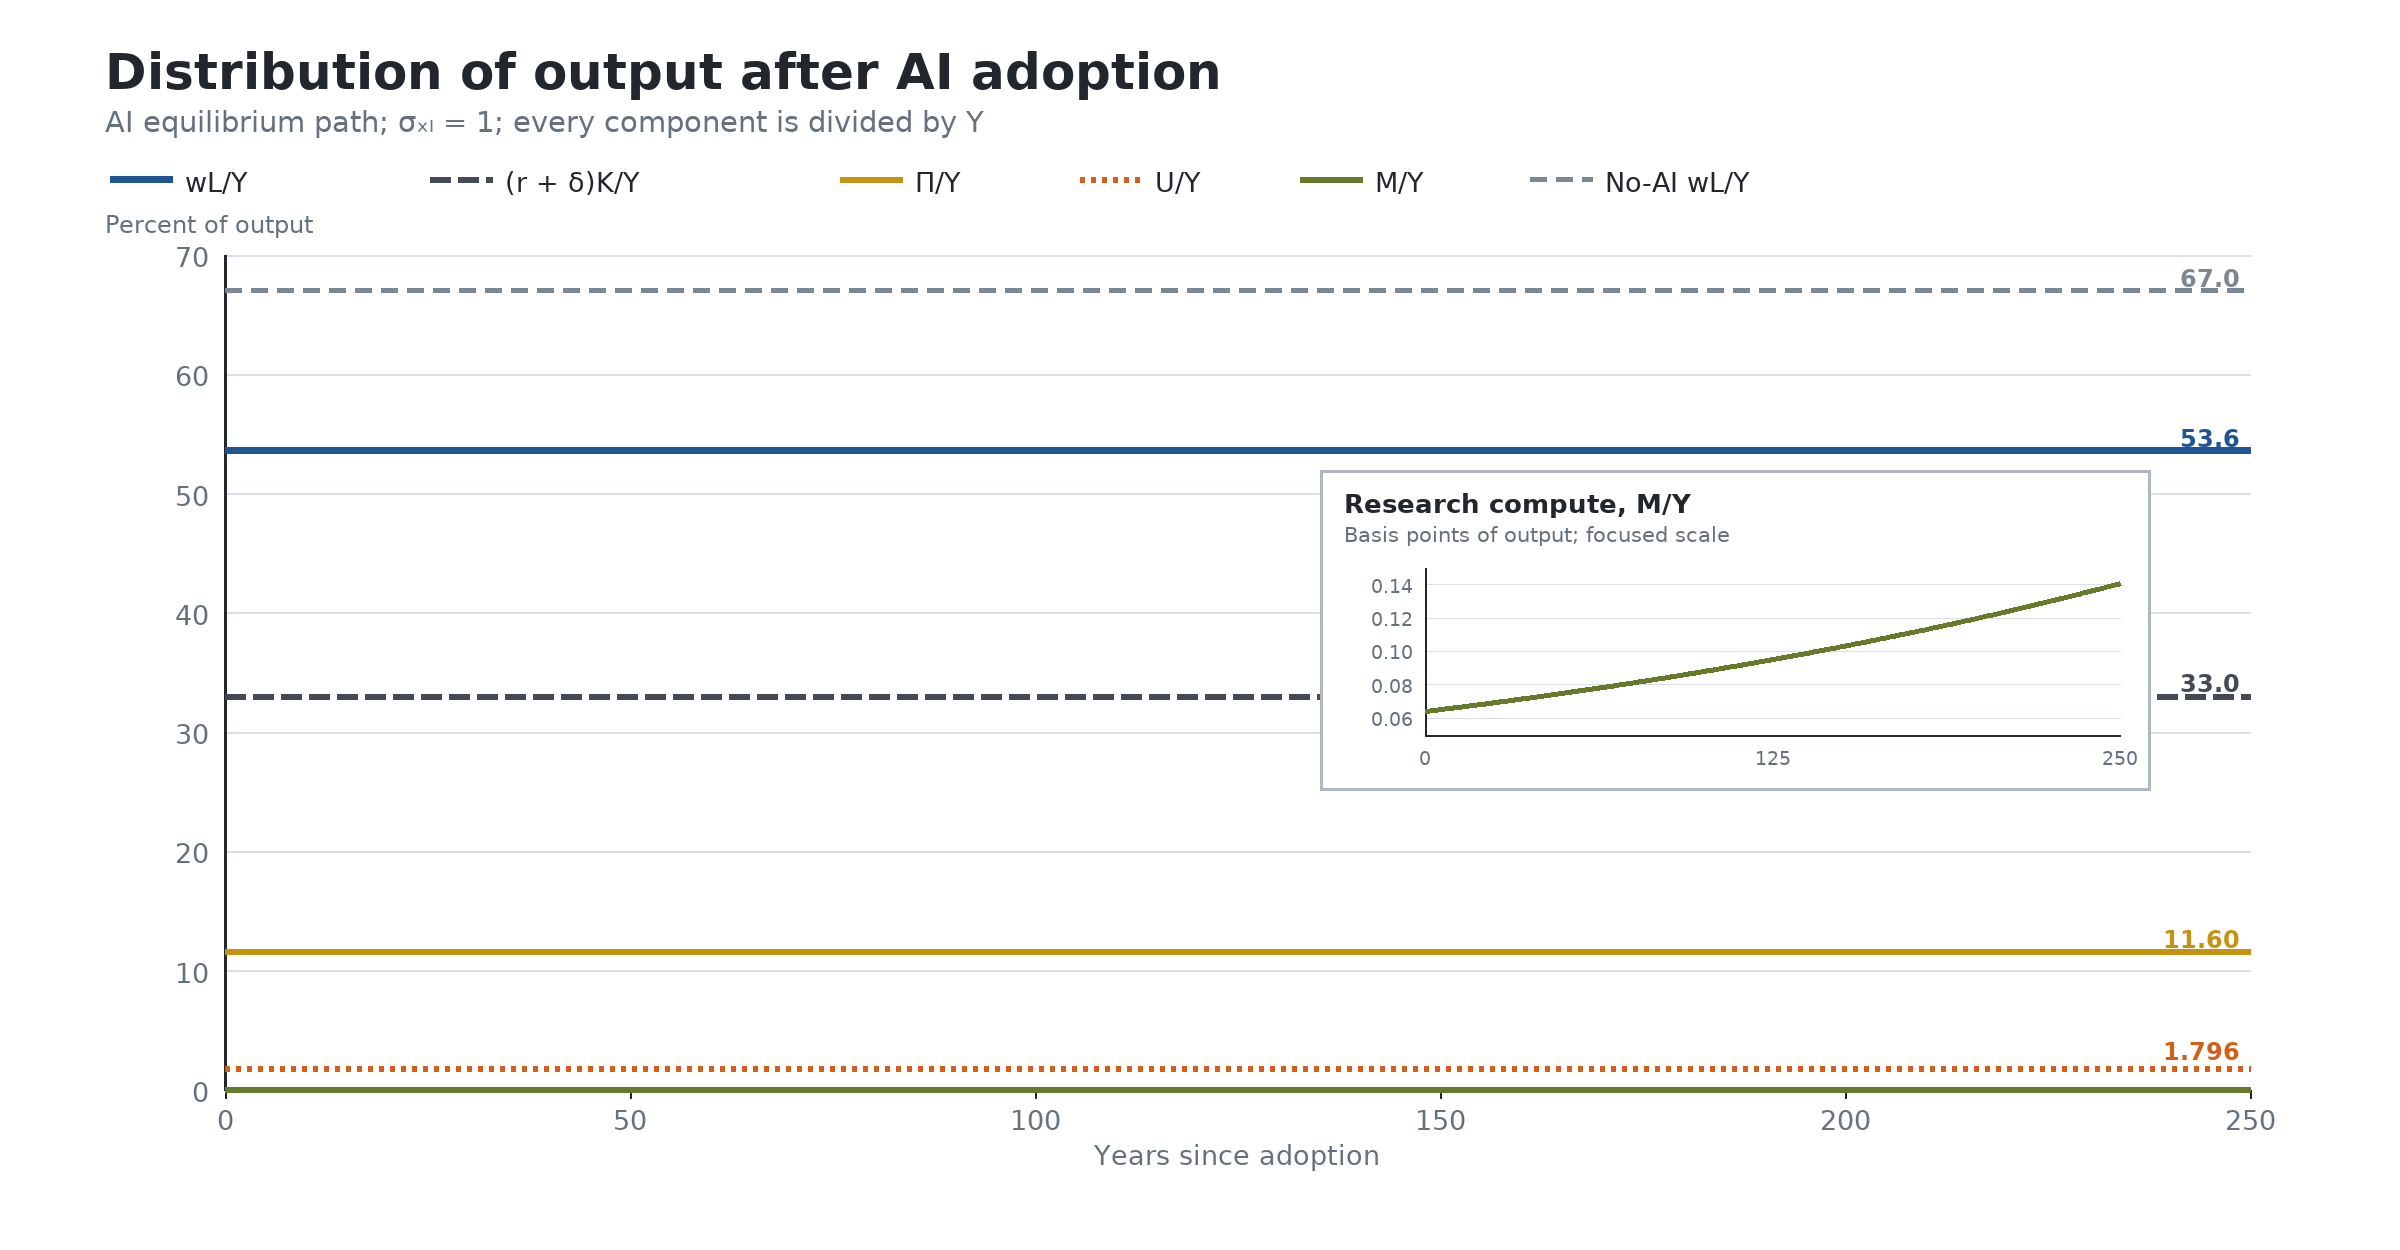
\includegraphics[width=\textwidth]{figures_axm/axm_ai_adoption_income_shares.png}
\caption{Trajectories of the consolidated output decomposition after AI
adoption. Every AI component is divided by \(Y\), and the five components sum
to one at every date. The gray dashed line reports the no-AI labor share as a
reference. The main panel uses percentage points on a linear scale. The inset
shows the same \(M/Y\) trajectory in basis points because it is too small to
read on the common scale. Since \(U\) and \(M\) are resource costs, this is a
consolidated decomposition of output rather than a factor-income decomposition
alone.}
\label{fig:axm-ai-adoption-distribution-paths}
\end{figure}

\subsubsection{\texorpdfstring{Case II: human-essential research, \(\sigma_{HM}=1\)}{Case II: human-essential research, sigma HM = 1}}
\label{sec:axm-case-human-essential}

When \(\sigma_{XL}=\sigma_{HM}=1\), the limiting share of research expenditure
allocated to AI research services is \(\bar s=\omega_M\). A balanced-growth candidate
therefore requires \(D(\omega_M)>0\) and the remaining feasibility conditions in
Proposition \ref{prop:axm-cd-bgp}. Human research and population grow at the same
rate, so \(H/N\) converges to a positive constant. The quantity of AI
research services can nevertheless grow faster than human research; human input
remains essential even as its quantity becomes small relative to \(BM\).

\subsubsection{\texorpdfstring{Case III: substitutable research, \(\sigma_{HM}>1\)}{Case III: substitutable research, sigma HM > 1}}
\label{sec:axm-case-substitutable-research}

When \(\sigma_{XL}=1\), \(\sigma_{HM}>1\), and the relative-price condition in
Proposition \ref{prop:axm-research-automation} holds, \(s_M\to1\) and the relevant
feedback denominator is \(D(1)\). A balanced-growth candidate therefore requires
\(D(1)>0\) and the remaining feasibility conditions in Proposition
\ref{prop:axm-cd-bgp}. Relative to Case II, automation strengthens the feedback
from capability to research. Human research grows more slowly than population and
\(H/N\) tends to zero on the candidate path.

\subsubsection{Numerical status}

The existing finite-horizon calculations comparing \(\sigma_{HM}=1\) and
\(\sigma_{HM}=2\) satisfy the dated equations, but their audit does not
establish an admissible infinite-horizon continuation satisfying both
transversality conditions. I therefore do not report their trajectories. The
analytical balanced-growth equilibria and local saddle-path results above remain
valid. A transition figure will be added only after the algorithm passes the
same equilibrium-admission test used for the benchmark paths.

\subsection{\texorpdfstring{Case IV: gross substitution in final production, \(\sigma_{XL}>1\)}{Case IV: gross substitution in final production, sigma XL > 1}}
\label{sec:axm-case-gross-substitution}

\subsubsection{Analytical characterization}

Let
\begin{equation}
 \theta=\frac{1-\alpha}{\alpha}.
 \label{eq:axm-theta}
\end{equation}
For \(\sigma_{XL}>1\), the static equilibrium conditions imply the exact
identity
\begin{equation}
 \frac{Y}{K}=B^\theta
 \left[
  (1-\alpha)s_X(1-e_X)
  \left(\frac{\omega_X}{s_X}\right)^{
   \sigma_{XL}/(\sigma_{XL}-1)}
 \right]^\theta.
 \label{eq:axm-high-sigma-exact-z}
\end{equation}
The expression in square brackets is continuous and strictly positive for
\(s_X\in(0,1]\), and it diverges as \(s_X\downarrow0\). It therefore has a
strictly positive lower bound. Hence \(B\to\infty\) implies
\(Y/K\to\infty\) even before establishing that AI production services dominate
the CES aggregate.

Along an interior branch on which \(s_X\to1\), AI production services do
eventually dominate that aggregate. Combining the same static conditions gives
\begin{equation}
 \frac{U}{Y}\to(1-\alpha)^2,\qquad
 \frac{Y}{K}\sim \mathcal D B^\theta
 \label{eq:axm-high-sigma-scaling}
\end{equation}
for a positive constant \(\mathcal D\).

\subsubsection{Finite-cap equilibrium regularization}
\label{sec:axm-finite-cap-gross-substitutes}

I now apply the finite-cap construction in Section
\ref{sec:axm-finite-cap-regularization}. The purpose is to replace the
finite-time boundary by an infinite-horizon economy for each
\(\overline B<\infty\), characterize that economy's terminal regime, and then
examine whether those equilibria have a meaningful limit as
\(\overline B\to\infty\).

For \(\sigma_{XL}>1\), define
\begin{equation}
 \mathcal D_\sigma=
 \left[(1-\alpha)^2
 \omega_X^{\sigma_{XL}/(\sigma_{XL}-1)}\right]^\theta,
 \qquad
 z_A(\overline B)=\mathcal D_\sigma\overline B^\theta,
 \label{eq:axm-capped-ai-only-productivity}
\end{equation}
where \(z_A(\overline B)\) is the limiting output--capital ratio when AI
production services dominate and capability is fixed at the frontier. Recall
\(\mathcal R=(\rho+\gamma_A+\delta)/\alpha\). The critical frontier is
\begin{equation}
 \overline B_c=
 \left(\frac{\mathcal R}{\mathcal D_\sigma}\right)^{1/\theta}.
 \label{eq:axm-critical-capability-frontier}
\end{equation}

To state the result, let
\begin{equation}
 \mathcal H_\sigma(s)=
 \left[
  (1-\alpha)s
  \left(1-\frac{1-s}{\sigma_{XL}}-\alpha s\right)
  \left(\frac{\omega_X}{s}\right)^{
   \sigma_{XL}/(\sigma_{XL}-1)}
 \right]^\theta.
 \label{eq:axm-capped-share-map}
\end{equation}
Equation \eqref{eq:axm-high-sigma-exact-z} is
\(Y/K=B^\theta\mathcal H_\sigma(s_X)\). The function
\(\mathcal H_\sigma\) is strictly decreasing on \((0,1]\), diverges as
\(s\downarrow0\), and satisfies
\(\mathcal H_\sigma(1)=\mathcal D_\sigma\).

\begin{proposition}[Terminal regimes of the finite-cap economy]
\label{prop:axm-capped-terminal-regimes}
Suppose \(\sigma_{XL}>1\), \(n+\gamma_A>0\), and \(\rho>n\). Consider a
regular finite-cap benchmark equilibrium that approaches
\(B=\overline B\), has convergent terminal ratios and growth rates, and has a
positive limiting consumption--output ratio.

If \(\overline B<\overline B_c\), the terminal regime is labor supported.
There is a unique \(\bar s_X\in(0,1)\) satisfying
\begin{equation}
 \mathcal R=\overline B^\theta\mathcal H_\sigma(\bar s_X).
 \label{eq:axm-capped-labor-supported-share}
\end{equation}
The limiting net interest rate and aggregate growth rate are
\begin{equation}
 \bar r=\rho+\gamma_A,\qquad
 \bar g=n+\gamma_A,\qquad
 \frac{wL}{Y}\to(1-\alpha)(1-\bar s_X)>0.
 \label{eq:axm-capped-labor-supported-rates}
\end{equation}

If \(\overline B>\overline B_c\), capital and AI production services outgrow
effective labor. The terminal regime is AI dominated and
\begin{align}
 \frac{Y}{K}&\to z_A(\overline B),&
 \bar r&=\alpha z_A(\overline B)-\delta,&
 \bar g&=n+\bar r-\rho>n+\gamma_A,
 \label{eq:axm-capped-ai-growth}\\
 \frac{wL}{Y}&\to0,&
 \frac{U}{Y}&\to(1-\alpha)^2,&
 \frac{p_XX}{Y}&\to1-\alpha.
 \label{eq:axm-capped-ai-shares}
\end{align}
The knife-edge \(\overline B=\overline B_c\) separates the two normalizations
and is not covered by the local terminal characterization.
\end{proposition}

The finite frontier therefore does not necessarily restore a positive labor
income share. It removes finite-time divergence, but a sufficiently high
frontier produces a finite-rate \(AK\)-type terminal regime in which labor
becomes asymptotically negligible. The rate is finite for every fixed
\(\overline B\), rather than uniformly bounded across frontiers.

\begin{proposition}[Research along a regular frontier approach]
\label{prop:axm-capped-frontier-research}
Maintain the conditions of Proposition
\ref{prop:axm-capped-terminal-regimes}. Suppose also that research compute and
the shadow value relative to output have positive finite limits and that the
frontier approach is regular. Let \(\bar g\) denote the terminal aggregate
growth rate in the relevant regime. Then
\begin{align}
 \frac{\dot B}{\overline B-B}&\to\bar g,&
 M&\to\overline M(\overline B)
 =\left[
  \frac{\bar g\,\overline B^{1-\eta}}{\chi}
 \right]^{1/\eta},
 \label{eq:axm-capped-terminal-research}\\
 g_q&\to\bar g,&
 \frac{X}{qB^2}&\to\bar r,&
 \frac{M}{Y}&\to0.
 \label{eq:axm-capped-terminal-shadow-value}
\end{align}
Both transversality objects have asymptotic log growth \(n-\rho<0\).
\end{proposition}

Combining Proposition \ref{prop:axm-capped-frontier-research} with the
developer's profit identity and the resource constraint completes the
consolidated decomposition in the AI-dominated regime:
\begin{equation}
 \frac{\Pi}{Y}\to\alpha(1-\alpha),\qquad
 \frac{C}{Y}\to
 \alpha(1-\alpha)+\frac{\rho-n}{z_A(\overline B)}.
 \label{eq:axm-capped-ai-consolidated-shares}
\end{equation}

These propositions characterize terminal restrictions for a finite-cap
equilibrium; they do not turn a solution of the capped dated equations into an
equilibrium automatically. A reported transition must still satisfy Definition
\ref{def:axm-benchmark-equilibrium}, including agent optimality and both
transversality conditions. Proposition
\ref{prop:axm-capped-developer-sufficiency} supplies a checkable developer
sufficiency condition near the frontier.

\begin{proposition}[The infinite-frontier limit]
\label{prop:axm-infinite-frontier-limit}
Suppose \(\sigma_{XL}>1\). On every compact subset of the positive state
space, the finite-cap state law, research condition, and costate equation
converge in \(C^1\) to their uncapped counterparts as
\(\overline B\to\infty\). Consequently, consider a sequence of finite-cap
equilibria for which \(\overline B_j\to\infty\), the selected initial jump
variables \((C_{0,j},q_{0,j})\) converge to a positive finite pair, and the
paths remain in a common compact subset on \([0,T]\). Their restrictions to
\([0,T]\) converge to the uncapped canonical path with the limiting initial
values. This finite-window statement does not establish that the sequence of
finite-cap equilibria exists or that its limit satisfies the uncapped
infinite-horizon transversality conditions.

The terminal regimes do not have a finite-rate limit. Once
\(\overline B>\overline B_c\),
\begin{equation}
 \bar r(\overline B)
 =\alpha\mathcal D_\sigma\overline B^\theta-\delta,\qquad
 \bar g(\overline B)
 =n-\rho-\delta+\alpha\mathcal D_\sigma\overline B^\theta,
 \label{eq:axm-capped-diverging-rates}
\end{equation}
so both rates diverge as \(\overline B\to\infty\). Hence taking the frontier
to infinity on a fixed pre-singular window is not the same operation as first
following each finite-cap equilibrium to its long run and then taking
\(\overline B\to\infty\).
\end{proposition}

The finite cap is therefore an equilibrium regularization of the pre-singular
branch, not a proof that the uncapped economy has an infinite-horizon
equilibrium. If capped equilibria can be constructed from the paper's initial
stocks, their limit can justify uncapped allocations on every compact interval
strictly before the singular date. It cannot supply an allocation at or beyond
that date.

Proposition \ref{prop:axm-research-burst} explains why the baseline uses the
stronger curvature restriction \(\eta<\alpha\). For all positive CES
elasticities and on each fixed regular horizon, the restriction makes the
developer's objective coercive over all nonnegative research policies with
finite expenditure and gives a finite truncated value. For the gross-substitutes
case in both nests studied here, the fixed-duration deviation establishes the
converse unboundedness result when \(\eta>\alpha\); the boundary
\(\eta=\alpha\) is not fully characterized.
The proposition does not supply compactness, prove that the finite-horizon
supremum is attained, establish a global or infinite-horizon optimum, select a
particular branch, or provide an admissible continuation through a finite-time
singularity.

\begin{proposition}[No finite-rate balanced growth with gross substitution]
\label{prop:axm-no-bgp}
Suppose \(\sigma_{XL}>1\), \(B\to\infty\), and an interior path satisfies the
dated equilibrium conditions. Then there is no balanced-growth path with finite
constant growth rates. In particular, \(Y/K\to\infty\), so the marginal product
of capital, the net interest rate, and household consumption growth become
unbounded.
\end{proposition}

The proposition is a conditional nonexistence result. It does not prove that every
initial condition enters the assumed unbounded-capability branch: capability may
remain bounded, a globally admissible continuation may fail, or the
infinite-horizon problem may not admit an optimum. The next result characterizes
the accelerating branch when it exists.

The bounded-capability alternative can be restricted without assuming that
normalized quantities or growth rates converge.

\begin{proposition}[No bounded capability with a bounded return]
\label{prop:axm-no-bounded-capability-tail}
Suppose the automated-research benchmark applies,
\(\sigma_{XL}>1\), \(n+\gamma_A>0\), and \(0<\eta<1\). There is no regular
interior infinite-horizon candidate satisfying the dated benchmark conditions
with both \(\sup_{t\geq0}B_t<\infty\) and
\(\sup_{t\geq0}r_t<\infty\).
\end{proposition}

\begin{proof}
Let \(\mathcal L=AN\) and \(G=n+\gamma_A>0\). Because capability is
nondecreasing, bounded capability implies
\(B_t\in[B_0,\bar B]\). Integrating its law gives
\begin{equation}
 B_t^{1-\eta}=B_0^{1-\eta}
 +(1-\eta)\chi\int_0^t M_s^\eta\dd s.
 \label{eq:axm-bounded-capability-integral}
\end{equation}
Hence \(\int_0^\infty M_t^\eta\dd t<\infty\). The research first-order
condition gives
\[
 M_t^\eta=(\chi\eta B_t^\eta)^{\eta/(1-\eta)}
 q_t^{\eta/(1-\eta)},
\]
so, because \(B_t\geq B_0>0\),
\begin{equation}
 \int_0^\infty q_t^{\eta/(1-\eta)}\dd t<\infty.
 \label{eq:axm-bounded-capability-q-integral}
\end{equation}

Now suppose \(r_t\leq\bar r\). The CES aggregate is bounded below by a
positive multiple of \(\mathcal L\). The capital-demand condition therefore
implies that \(K/\mathcal L\) is bounded away from zero. Homogeneity and the
unique static monopoly solution then give a uniform constant
\(\underline x>0\) such that
\(X_t/\mathcal L_t\geq\underline x\). In levels, the costate equation is
\[
 \dot q=a_tq-\frac{X}{B^2},\qquad
 a_t=r_t-\eta g_{B,t}\leq\bar r.
\]
Solving this linear equation backward from \(t+1\) to \(t\), using
\(q_{t+1}>0\), yields
\[
 q_t\geq\int_t^{t+1}
 e^{-\int_t^s a_v\dd v}\frac{X_s}{B_s^2}\dd s
 \geq c e^{Gt}
\]
for a constant \(c>0\). This contradicts
\eqref{eq:axm-bounded-capability-q-integral}. Therefore bounded capability and
a bounded return cannot coexist on such a candidate.
\end{proof}

The result is stronger than a stationary-limit argument, but it deliberately
leaves open a bounded-capability path with unbounded interest-rate spikes. The
next proposition records restrictions that every remaining irregular
continuation must satisfy.

\begin{proposition}[Necessary restrictions on an irregular gross-substitutes continuation]
\label{prop:axm-gross-substitutes-irregular-necessity}
Suppose the automated-research benchmark applies,
\(\sigma_{XL}>1\), \(n+\gamma_A>0\), and \(0<\eta<1\). Any regular interior
infinite-horizon equilibrium, if one exists, must satisfy one of the following:
\begin{enumerate}
 \item \(B\) is bounded and \(\sup_{t\geq0}r_t=\infty\); or
 \item \(B\to\infty\), and, writing \(z=Y/K\) and
 \(\theta=(1-\alpha)/\alpha\),
 \begin{equation}
  \liminf_{t\to\infty}\frac{g_{B,t}}{z_t}=0,
  \qquad
  \int_0^\infty e^{-(\rho-n)t}B_t^\theta\dd t<\infty.
  \label{eq:axm-irregular-necessary-restrictions}
 \end{equation}
\end{enumerate}
\end{proposition}

\begin{proof}
The first alternative follows from Proposition
\ref{prop:axm-no-bounded-capability-tail}. Suppose instead that \(B\to\infty\).
Equation \eqref{eq:axm-high-sigma-exact-z} gives
\(z_t\geq dB_t^\theta\) for some \(d>0\). If
\(\liminf g_B/z>0\), then eventually
\(\dot B=B g_B\geq\varepsilon dB^{1+\theta}\) for some
\(\varepsilon>0\), which makes \(B\) unbounded in finite time. An
infinite-horizon equilibrium must therefore satisfy the first restriction in
\eqref{eq:axm-irregular-necessary-restrictions}.

For the second, let \(c_h=C/N\). The household Euler equation gives
\[
 \log c_{h,t}=\log c_{h,0}-(\rho+\delta)t
 +\int_0^t(r_s+\delta)\dd s.
\]
Because \(r+\delta=\alpha z>0\), Tonelli's theorem shows that finiteness of the
household's improper utility integral requires
\[
 \int_0^\infty e^{-(\rho-n)t}(r_t+\delta)\dd t<\infty.
\]
Combining this condition with \(z_t\geq dB_t^\theta\) proves the second
restriction in \eqref{eq:axm-irregular-necessary-restrictions}.
\end{proof}

These restrictions do not assert that either irregular alternative exists.
They identify what a general nonexistence proof would still have to eliminate.
The next result characterizes the more regular unbounded AI-dominated
alternative.

\begin{conditionalresult}[AI-dominated singular limit]
\label{prop:axm-singular-limit}
Assume \(\sigma_{XL}>1\), \(0<\eta<\alpha<1\), and either the
automated-research benchmark or the human-research extension with
\(\sigma_{HM}>1\). Let an interior path satisfy all dated technology and service
identities, competitive price equations, static first- and second-order
conditions, market-clearing conditions, and canonical differential equations
on its maximal time interval. Suppose that the path approaches an AI-dominated
limit, with \(B\to\infty\) and \(s_X\to1\). In the human-research extension,
also suppose \(s_M\to1\); in the benchmark, set \(s_M\equiv1\). Suppose its
consumption, investment, and research-compute
shares---respectively \(C/Y\),
\((\dot K+\delta K)/Y\), and \(M/Y\)---as well as \(g_B/(Y/K)\) and \(qB/K\),
converge to positive finite limits.
Assume that the convergences of \(s_X\), \(s_M\), all the listed ratios, and the scaling ratio
\((Y/K)/(\mathcal D B^\theta)\to1\) are asymptotically regular: the growth rate
of each convergent ratio, divided by \(Y/K\), tends to zero. Write \(z=Y/K\) and
\[
 \Delta=1+\theta-\eta,\qquad
 h=\frac{\eta\alpha}{\Delta}.
\]
Then
\begin{align}
 \frac{g_B}{z}&\to h,&
 \frac{U}{Y}&\to(1-\alpha)^2,\\
 \frac{\dot K+\delta K}{Y}&\to\alpha-\theta h,&
 \frac{M}{Y}&\to\frac{\eta(1-\alpha)^2}{\Delta},\\
 \frac{qB}{K}&\to\frac{(1-\alpha)^2}{\eta\alpha},&
 \frac{C}{Y}&\to
 1-(1-\alpha)^2-\alpha+\theta h
 -\frac{\eta(1-\alpha)^2}{\Delta}.
 \label{eq:axm-singular-ratios}
\end{align}
Moreover,
\begin{equation}
 \dot z\sim\theta h z^2.
 \label{eq:axm-z-law}
\end{equation}
Because the limiting gross-investment share
\(\alpha-\theta h=\alpha(1-\eta)/(1-\alpha\eta)\) is positive, capital is
eventually increasing. Thus \(z\), and consequently output, become unbounded in
finite time.
For the wage result, define
\[
 \underline\sigma=
 \begin{cases}
  \sigma_{XL},&\text{in the automated-research benchmark},\\
  \min\{\sigma_{XL},\sigma_{HM}\},&\text{in the human-research extension}.
 \end{cases}
\]
In the human-research extension, the allocation of labor satisfies
\begin{equation}
 (H/N,L/N)\to
 \begin{cases}
  (1,0),&\sigma_{HM}<\sigma_{XL},\\
  (\bar h_N,1-\bar h_N),
      &\sigma_{HM}=\sigma_{XL}=\sigma,\\
  (0,1),&\sigma_{HM}>\sigma_{XL}.
 \end{cases}
 \label{eq:axm-singular-labor-allocation}
\end{equation}
In the equal-elasticity case, the limiting share is pinned down by
\begin{equation}
 \bar h_N=\frac{\mathcal R_\sigma}{1+\mathcal R_\sigma},\qquad
 \mathcal R_\sigma=\frac{\eta}{\Delta}A_*^{1-\sigma}
 \left[
  \frac{(1-\alpha)\omega_H\omega_X}{\omega_M\omega_L}
 \right]^{\sigma}.
 \label{eq:axm-singular-equal-elasticity-share}
\end{equation}
Here \(A_*=\lim_{t\uparrow T^*}A_t\) is finite and positive because labor
productivity grows exogenously and the singular date is finite.
In the benchmark, \(L=N\). In both versions, production labor income,
\(wL/Y\), and aggregate labor income, \(wN/Y\), vanish as shares of output,
while
\begin{equation}
 \frac{g_w}{z}\to
 \frac{\alpha-(\underline\sigma-1)h}{\underline\sigma}
 \label{eq:axm-wage-limit}
\end{equation}
which is positive if and only if
\(\underline\sigma<1/(\alpha\eta)\).
\end{conditionalresult}

\begin{proposition}[No regular benchmark continuation]
\label{prop:axm-no-regular-gross-substitutes-continuation}
Suppose the automated-research benchmark applies, \(\sigma_{XL}>1\),
\(0<\eta<\alpha<1\), and \(n+\gamma_A>0\). Consider a regular interior
candidate whose proposed long-run continuation belongs to either of the two
classes used by the algorithm:
\begin{enumerate}
 \item capability and the interest rate are bounded; or
 \item capability is unbounded and the conditions of Conditional Result
 \ref{prop:axm-singular-limit} hold.
\end{enumerate}
Neither continuation can complete the candidate as an admissible
infinite-horizon equilibrium.
\end{proposition}

\begin{proof}
The first continuation contradicts the developer's costate equation by
Proposition \ref{prop:axm-no-bounded-capability-tail}. Under the second,
Conditional Result \ref{prop:axm-singular-limit} gives
\(\dot z\sim\theta h z^2\), where \(z=Y/K\) and \(\theta h>0\). The maximal
path therefore ends at a finite singular date and is not defined for every
\(t\geq0\). Proposition \ref{prop:axm-no-zero-research-corner} also shows that
setting \(M=0\) at a finite date cannot rescue either continuation.
\end{proof}

Conditional Result \ref{prop:axm-singular-limit} characterizes a postulated
asymptotic branch of the model's necessary
conditions. Because the maximal interval ends at the singularity, it does not
establish existence or global optimality for the infinite-horizon problems, nor
does it establish that the branch is reached from arbitrary initial conditions.
Proposition \ref{prop:axm-no-regular-gross-substitutes-continuation} is an
exhaustion result only within the two regular terminal classes stated there. It
does not exclude either irregular alternative in Proposition
\ref{prop:axm-gross-substitutes-irregular-necessity}: bounded capability with
unbounded interest-rate spikes, or unbounded capability with
\(\liminf g_B/(Y/K)=0\) and sufficiently slow discounted growth. Nor does it
exclude another terminal regime not used by the algorithm.
Within that branch, workers move asymptotically toward the sector in which they
are harder to replace. The model delivers a sharp separation when
\(1<\underline\sigma<1/(\alpha\eta)\): aggregate labor income as a share of output
vanishes, but the wage eventually rises. Above the threshold, the same conditional
scaling implies an eventually falling wage. The case above the threshold should
not be interpreted without separately
checking monopoly optimality and convergence to the postulated branch.
At \(\underline\sigma=1/(\alpha\eta)\), the leading term in
\eqref{eq:axm-wage-limit} is zero, so this asymptotic calculation alone does not
determine the eventual direction of the wage.

The growth-rate transformation used by \citet{davidsonetal2026} provides a useful
interpretation of this conditional branch. The limiting ratios imply
\[
 \dot B\sim \kappa_B B^{\eta(1+\theta)}K^\eta,
 \qquad
 \dot K\sim \kappa_K B^\theta K
\]
for positive constants \(\kappa_B,\kappa_K\). Hence the growth rates satisfy
\begin{equation}
 \begin{pmatrix}
  \dot g_B/g_B\\[2pt] \dot g_K/g_K
 \end{pmatrix}
 \sim
 \underbrace{\begin{pmatrix}
  \eta(1+\theta)-1&\eta\\
  \theta&0
 \end{pmatrix}}_{\Omega_\infty}
 \begin{pmatrix}g_B\\g_K\end{pmatrix}.
 \label{eq:axm-singular-feedback-matrix}
\end{equation}
Under Assumption \ref{ass:axm-large-scale-curvature}, the diagonal
\(g_B\)-feedback coefficient is negative:
\[
 \eta(1+\theta)-1=\frac{\eta}{\alpha}-1<0.
\]
Nevertheless,
\[
 \det\Omega_\infty=-\eta\theta<0,
\]
so \(\Omega_\infty\) has one positive and one negative eigenvalue. The positive
eigenvalue is generated by the off-diagonal two-way link between capability
growth and capital growth. Making the diagonal feedback subcritical does not
eliminate the positive direction created by the coupled feedback system. This is
the matrix counterpart of \(\dot z\sim\theta h z^2\) on the postulated branch;
it does not establish global optimality, reachability, or an admissible
continuation beyond the finite-time boundary.

\subsubsection{Why no gross-substitutes trajectory is reported}

For \(\sigma_{XL}=1.01\), the algorithm follows the continuation order used on
the two sides of one: it starts from the exact strictly positive-AI
unit-elastic equilibrium, changes \(\sigma_{XL}\) on a short horizon, and then
extends the horizon while preserving the same dated equations and initial
stocks. The initial consumption and shadow-value jumps stabilize, but this does
not identify an infinite-horizon continuation. At \(T=5{,}000\), the terminal AI share
is only \(0.2303\), far from the AI-dominated limit. The local separation rate
\((\sigma_{XL}-1)\eta(n+\gamma_A)/\sigma_{XL}\) is
\(4.29\times10^{-5}\), whose inverse is about 23,300 model years. Near-unit
finite-window similarity is therefore expected even though the long-run
regimes differ.

Proposition \ref{prop:axm-no-bounded-capability-tail} rejects bounded
capability whenever the interest rate is bounded. The regular
AI-dominated alternative is the finite-time branch in Conditional Result
\ref{prop:axm-singular-limit}, not an infinite-horizon allocation. Proposition
\ref{prop:axm-gross-substitutes-concavity-gate} also shows that the sufficient
global concavity condition fails over the full counterfactual capability
domain at every date: its limiting service-capability elasticity is
\(1/\alpha=3.03>2\) under the calibration. For \(\sigma_{XL}=1.01\), optimized
operating profit first loses concavity at \(s_X=0.7386\), above the terminal
share in the finite-window calculation. Thus the saved segment remains on the
locally concave part of the state space, but the sufficient theorem cannot
compare it with all admissible alternatives. This failure is not a
nonexistence proof, but it prevents the computed first-order-condition branch
from being admitted as a globally optimal developer policy.

The older free-boundary calculation for
\((\sigma_{XL},\sigma_{HM})=(1.5,2)\) likewise solves the dated necessary
conditions only up to a finite artificial boundary. Under the equilibrium
definition in Section \ref{sec:axm-model}, neither calculation constructs an
admissible path for every \(t\geq0\). I therefore report no simulated
trajectory for \(\sigma_{XL}>1\). Both calculations remain in the repository
as diagnostics for the conditional analytical result, not as sources of paper
figures.

\subsection{Factor payments and resource uses across regimes}
\label{sec:axm-distributional-accounting}

The regimes can now be compared using the same accounting of factor payments
and resource uses. Zero profit in the final-good sector implies
\begin{equation}
 1=\frac{(r+\delta)K}{Y}+\frac{wL}{Y}+\frac{p_XX}{Y}
 =\alpha+(1-\alpha)(1-s_X)+(1-\alpha)s_X.
 \label{eq:axm-final-sector-distribution}
\end{equation}
Thus \(\alpha\) is the gross capital-payment share, including depreciation, and
\(s_X\) determines how the remaining output is divided between production labor
and purchases of AI production services.

Gross revenue from AI production services is not developer profit:
\begin{equation}
 \frac{p_XX}{Y}=\frac{U}{Y}+\frac{wH}{Y}+\frac{M}{Y}+\frac{\Pi}{Y}.
 \label{eq:axm-developer-revenue-distribution}
\end{equation}
Inference compute, research wages, and research compute are paid before the
residual \(\Pi\) is distributed. Substituting this identity into the final firm's
accounts yields the six-part decomposition in
\eqref{eq:axm-consolidated-distribution} without counting \(p_XX\) twice.

The final-production elasticity does not determine these shares by itself at a
finite date because \(s_X\) also depends on the equilibrium ratio \(X/(AL)\). The
propositions above determine the following conditional limiting shares. Under
complementarity, for any \(0<\sigma_{XL}<1\) satisfying the hypotheses of Propositions
\ref{prop:axm-complements} and \ref{prop:axm-complements-research},
\begin{equation}
 \frac{wN}{Y}\longrightarrow
 \frac{\sigma_{XL}(1-\alpha)^2}{1-\alpha\sigma_{XL}},
 \qquad
 \frac{p_XX}{Y},\frac{\Pi}{Y}\longrightarrow
 \frac{(1-\alpha)(1-\sigma_{XL})}{1-\alpha\sigma_{XL}}.
 \label{eq:axm-complement-distribution}
\end{equation}
At unit elasticity, \(s_X=\omega_X\), so the final-good firm's gross payment
shares are constant. On the conditional AI-dominated gross-substitutes branch,
\(s_X\to1\), aggregate labor income vanishes relative to output, and gross
revenue from AI production services approaches \(1-\alpha\).

Table \ref{tab:axm-distributional-synthesis} reports the conditional limits for
the three \(\sigma_{HM}=2\) benchmarks. The first two rows use balanced-growth
limits or candidates; the last uses the conditional pre-singular ratios.

\begin{table}[H]
\centering
\footnotesize
\setlength{\tabcolsep}{3.5pt}
\caption{Payments and resource uses at the conditional limits of the three benchmark regimes}
\label{tab:axm-distributional-synthesis}
\begin{tabular}{lrrrrrr}
\toprule
Final-production regime & \((r+\delta)K/Y\) & \(wL/Y\) & \(wH/Y\) & \(\Pi/Y\) & \(U/Y\) & \(M/Y\)\\
\midrule
Complements, \(\sigma_{XL}=0.75\) & 33.000 & 44.741 & 0.000 & 22.259 & 0.000 & 0.000\\
Unit elasticity, \(\sigma_{XL}=1\) & 33.000 & 53.600 & 0.000 & 11.567 & 1.796 & 0.038\\
Gross substitutes, \(\sigma_{XL}=1.5\) & 33.000 & 0.000 & 0.000 & 18.938 & 44.890 & 3.172\\
\bottomrule
\end{tabular}

\medskip
\parbox{0.95\textwidth}{\footnotesize \emph{Notes:} Entries are percentages of
\(Y\). The six components sum to final output without counting the intermediate
payment for AI production services twice. Zeros are limiting shares, not zero quantities at every
finite date. The first two rows are balanced-growth limits or candidates; the
last is the conditional pre-singular limit, not a proved infinite-horizon
equilibrium.}
\end{table}

The equilibrium transition figures above report this decomposition only for
paths that pass the equilibrium-admission audit. I do not combine them with the
gross-substitutes free-boundary calculation, because that calculation is not an
infinite-horizon equilibrium trajectory. The conditional last row of Table
\ref{tab:axm-distributional-synthesis} is therefore an analytical benchmark,
not a simulated income-distribution path.

The net interest rate and the capital-income share are also different objects.
The gross capital-payment share remains \(\alpha\) in every regime, but
\begin{equation}
 \frac{rK}{Y}=\alpha-\delta\frac{K}{Y}.
 \label{eq:axm-net-capital-share}
\end{equation}
Under complementarity, \(r\to\rho\) and the net capital-income share converges
to \(\alpha\rho/(\rho+\delta)\). At unit elasticity, the Euler equation gives
\(r=\rho+g_{C/N}\). On the conditional gross-substitutes branch,
\(r=\alpha(Y/K)-\delta\to\infty\) while \(K/Y\to0\), so net capital income
approaches the same share \(\alpha\) as the gross payment. The return on each
unit of capital becomes unbounded without raising capital's gross payment above
\(\alpha Y\).

These regime limits should not be read as a continuous comparative-static curve
at \(\sigma_{XL}=1\). At every fixed finite date, the CES aggregate converges
continuously to Cobb--Douglas as \(\sigma_{XL}\to1\). What does not commute is
taking each branch's asymptotic limit first:
\begin{equation}
 \lim_{\sigma_{XL}\uparrow1}\bar s_X=0,
 \qquad s_X\big|_{\sigma_{XL}=1}=\omega_X,
 \qquad s_X\to1\ \text{on the AI-dominated branch for every }\sigma_{XL}>1.
 \label{eq:axm-noncommuting-distribution-limits}
\end{equation}
The table therefore compares distinct conditional regimes rather than tracing a
smooth long-run comparative-static curve in \(\sigma_{XL}\). The relevant local
question is different: if I perturb \(\sigma_{XL}\) slightly, how long does the
new path remain close to the unit-elastic path?

For a one-sided comparison of admitted paths, I set \(\omega_X=0.20\) and give
both economies the unit-elastic balanced-growth stocks \(K_0=K^*\) and
\(B_0=B^*\), with \(A_0=N_0=1\). At date zero, \(\sigma_{XL}\) is permanently
\(0.99\) or \(1\). The states are identical; \(C_0\) and \(q_0\) jump, and no
flow is rescaled. The \(0.99\) algorithm uses the complementary-input terminal
regime and verifies both transversality conditions; the unit path is the
analytical balanced-growth equilibrium. I exclude \(1.01\) because its
unit-elastic terminal projection does not establish an admissible
infinite-horizon equilibrium. For \(0.99\), the separate optimality audit also
checks Proposition \ref{prop:axm-path-specific-sufficiency} over every
capability level \(B\geq B_0\), rather than applying the unit-elasticity
sufficiency proposition outside its domain.

\begin{figure}[H]
\centering
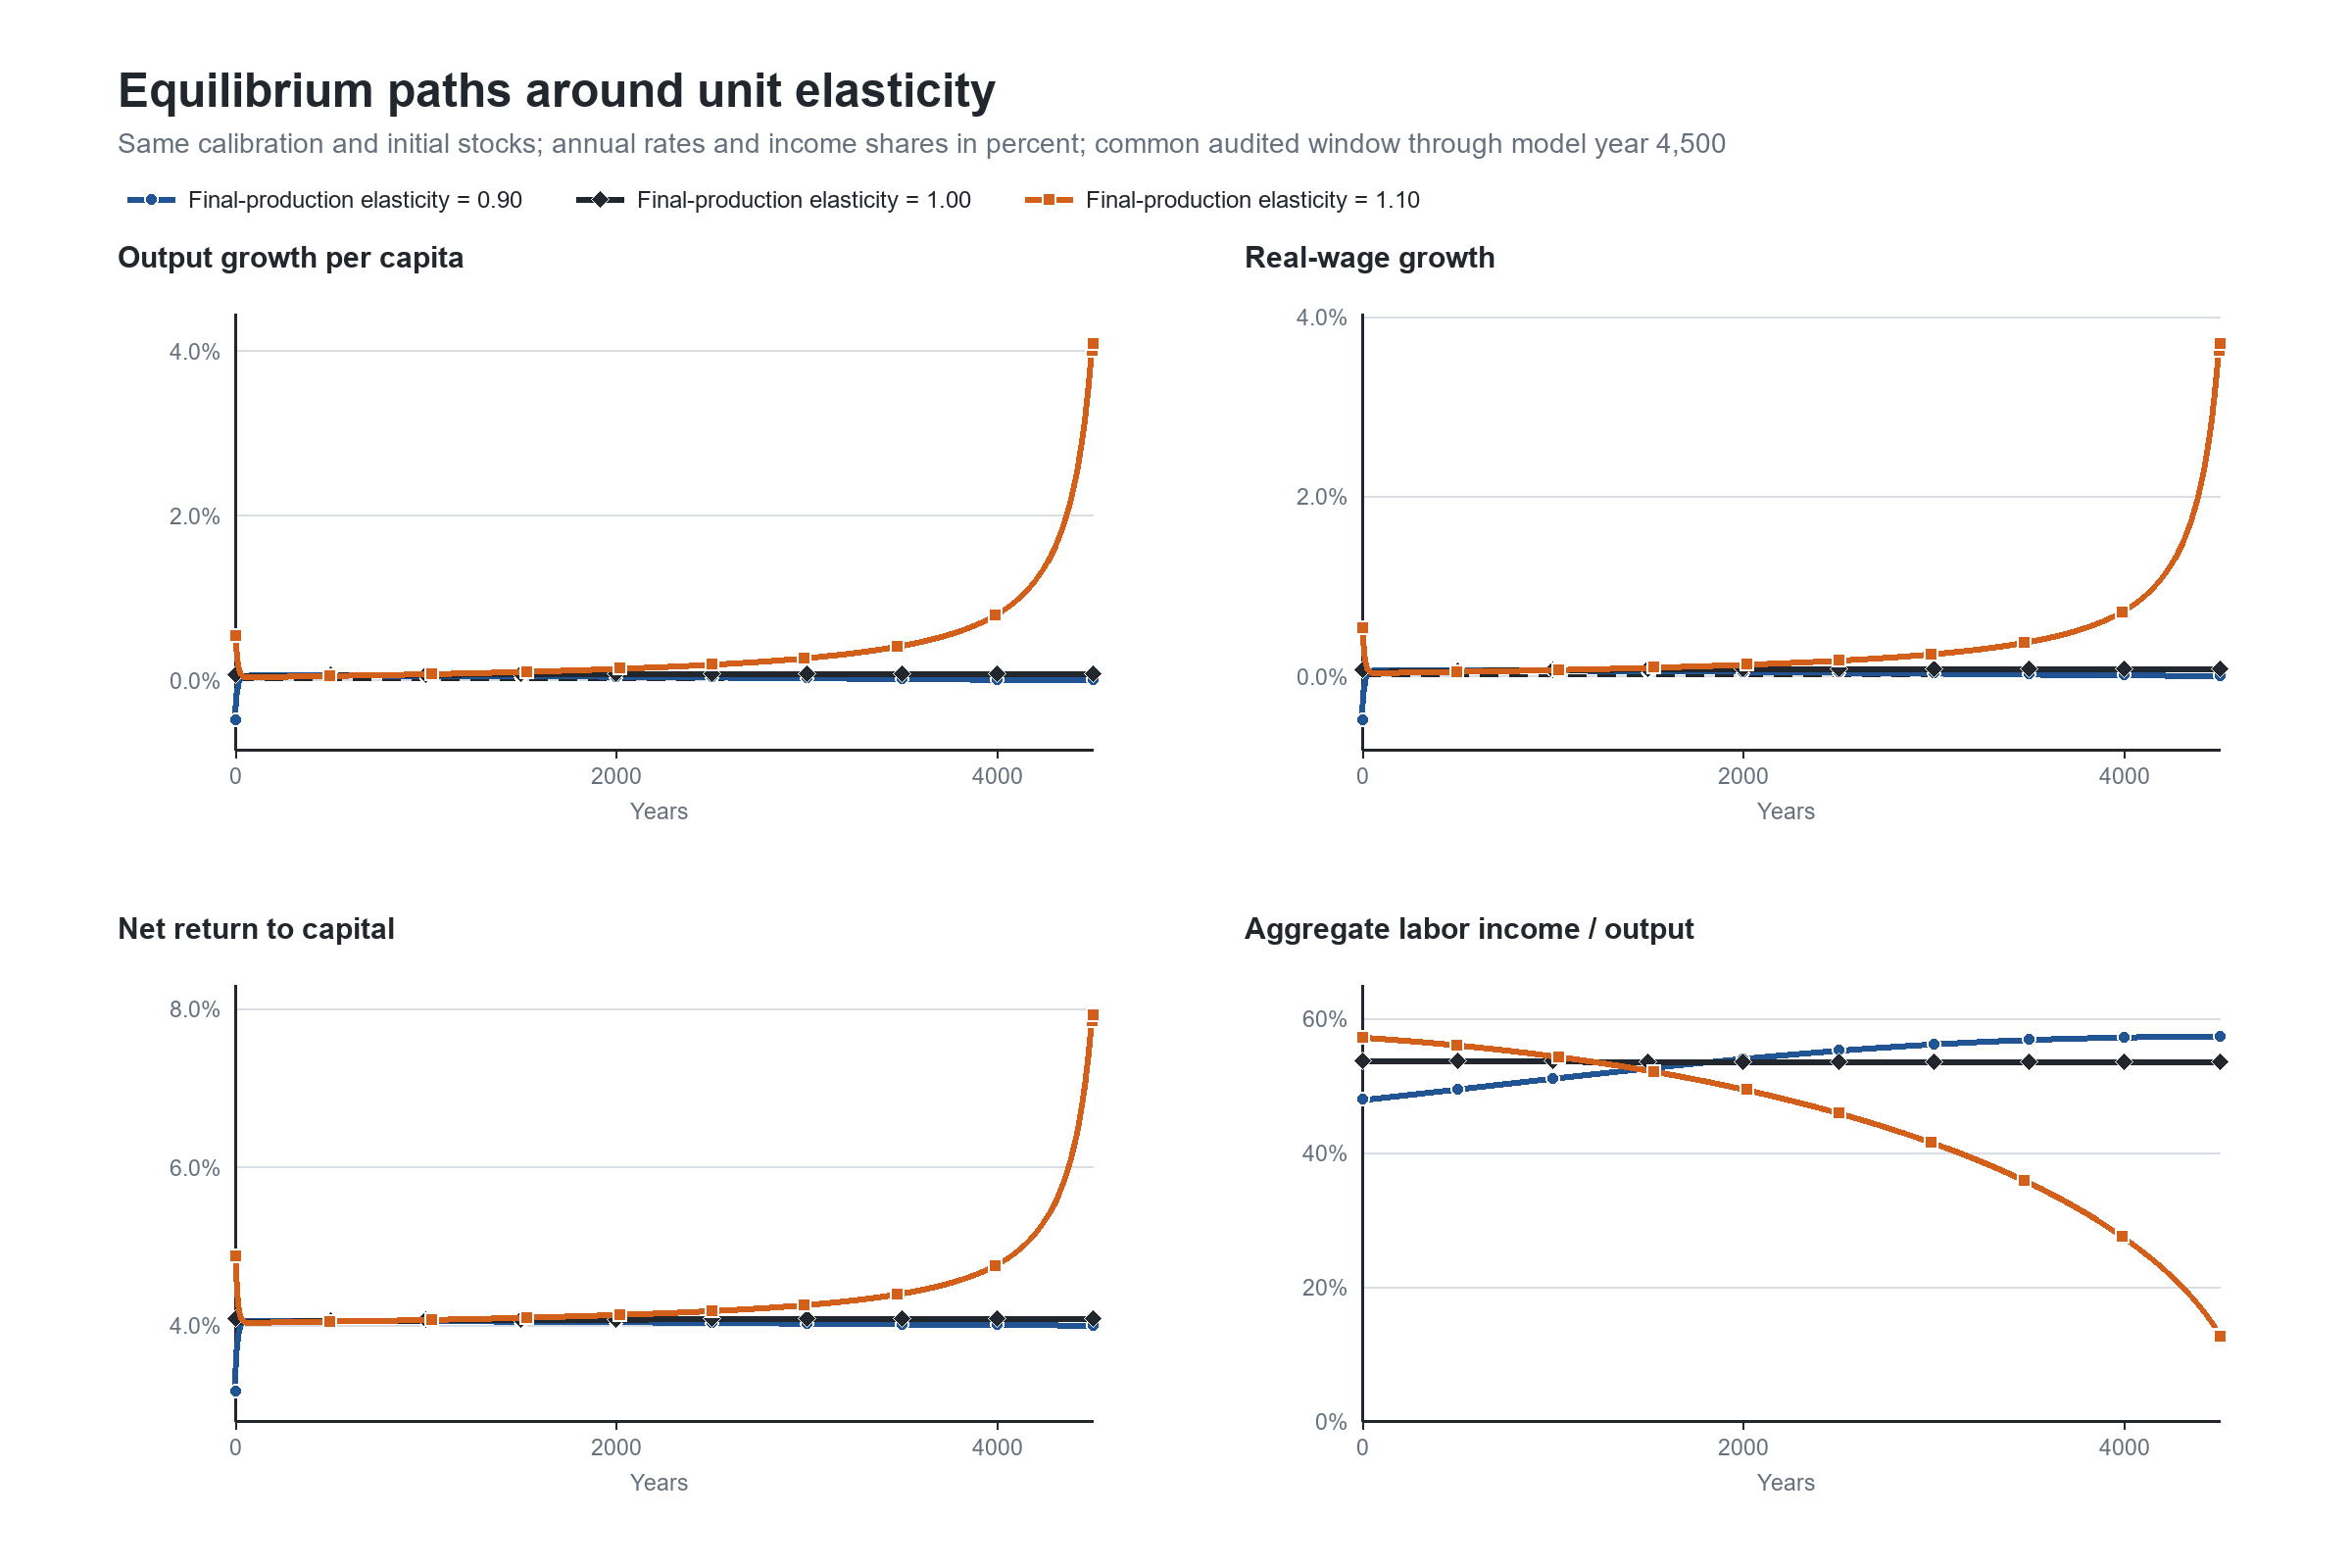
\includegraphics[width=\textwidth]{figures_axm/axm_near_unit_equilibrium_paths.png}
\caption{Admitted near-unit equilibrium trajectories from common unit-elastic
balanced-growth stocks. In both cases \(\omega_X=0.20\). The
\(\sigma_{XL}=0.99\) terminal audit extends through year 12,000, but I show only
years 0--2,500. The output and wage panels report 100 times the log difference
from the \(\sigma_{XL}=1\) equilibrium; the other panels report annual
percentages. Appendix \ref{app:axm-near-unit-equilibrium-paths} describes the
regime-specific terminal and admission tests.}
\label{fig:axm-near-unit-equilibrium}
\end{figure}

The initial distributional response reflects the fact that the common starting
stocks imply \(X/(AL)<1\). Equation
\eqref{eq:axm-near-unit-share-expansion} implies that lowering
\(\sigma_{XL}\) initially raises \(s_X\) and lowers labor's income share. As
\(X/(AL)\) grows, this ordering reverses. By year 2,500, 100 times the log gaps
in output per person and the real wage are \(-7.68\) and \(-6.64\),
respectively. Labor receives 54.16 percent of output, compared with 53.60
percent at unit elasticity, while the net interest rate remains close to its
unit-elastic value.

This experiment documents one-sided finite-date continuity between two admitted
equilibria, not similarity of their long-run paths. For a fixed nonunit
elasticity,
\(h=\varphi\ln[X/(AL)]\) accumulates over time and eventually becomes
economically important. Thus the limits \(\sigma_{XL}\to1\) and
\(t\to\infty\) need not commute. The regime propositions, rather than this
finite-window comparison, characterize the conditional long-run regimes. A
bilateral equilibrium comparison around one remains incomplete until an
admissible \(\sigma_{XL}>1\) equilibrium is constructed. Proposition
\ref{prop:axm-no-regular-gross-substitutes-continuation} rejects both regular
continuations used by the algorithm, so the admission rule rejects the computed
finite-window path instead of presenting it as an equilibrium.

Finally, these are functional distribution results, not predictions about
interpersonal inequality. The representative household supplies all labor and
owns both physical capital and the developer. A vanishing labor-income share
also need not imply a falling real wage: along the conditional gross-substitutes
branch, the wage can rise while \(wN/Y\) falls because output grows faster than
labor income.

\subsection{Cross-regime synthesis and limits of the evidence}

The feedback mechanism differs across regimes. Complementarity keeps \(X/(AL)\)
finite because raw inference compute falls as capability rises. Unit elasticity
produces the constant limiting matrix \(\mathcal F(\bar s)\). Gross substitution
makes the feedback state dependent; on the conditional AI-dominated branch it is
summarized by \(\Omega_\infty\). These are distinct economic regimes rather than
small perturbations around Cobb--Douglas.

The propositions characterize limits under their stated hypotheses. The
reported simulations are restricted to the complementary-input and
unit-elasticity trajectories that pass the equilibrium-admission rule. The
gross-substitutes free-boundary calculation remains a diagnostic of a
conditional pre-singular solution of the necessary conditions; it is not
reported as an equilibrium trajectory and does not establish global optimality
or selection of that branch from arbitrary initial states.

\section{Conclusion}

I develop an endogenous-growth model in which AI capability makes compute more
productive both in current production and in AI research. This creates two
feedback loops. The technological loop runs from capability to more effective
research compute and back to capability. The economic loop runs from capability
to output, accumulation, and research expenditure. Following the logic of
\citet{davidsonetal2026}, the strength of these loops depends not only on
technology but also on equilibrium prices and allocations.

The first result concerns the developer's research problem. On every finite
horizon, \(\eta<\alpha\) makes the objective coercive in total research
expenditure and keeps its value finite. When both CES technologies permit gross
substitution, \(\eta>\alpha\) instead allows research-compute expansions that
make the value unbounded. The benchmark \(\eta=0.20<\alpha=0.33\) is therefore a
deliberate regularity restriction, not an empirical estimate. Coercivity is
necessary for a well-behaved problem, but it does not by itself prove existence
of a global optimum or an infinite-horizon equilibrium.

The final-production elasticity then organizes the macroeconomic results. When
labor and AI production services are complements, labor remains a bottleneck and
capability creates no per-capita growth beyond exogenous labor productivity. In
the reported case with zero exogenous productivity growth, output per person
converges to a constant even though capability continues to improve. At unit
elasticity, the automated-research benchmark admits an equilibrium
balanced-growth path under explicit restrictions, and the calibration has the
local saddle-path structure needed for transition equilibrium from nearby
stocks. In the human-research extension, the corresponding growth restrictions
remain necessary rather than sufficient. The reciprocal of the feedback
denominator is the scalar counterpart of the feedback multiplier in
\citet{davidsonetal2026}. When labor and AI production services
are gross substitutes and AI production services dominate the final-production composite,
\(Y/K\) and the return to capital become unbounded, so no finite-rate
balanced-growth path can describe that branch.

These regimes also have sharply different implications for factor payments and
resource use. The outer Cobb--Douglas technology fixes the final-good firm's
gross capital payment
at \(\alpha Y\), including depreciation. What changes with \(\sigma_{XL}\) is
the division of the remaining output between production labor and purchases of
AI production services. Those purchases are not developer profit: they finance inference
compute, human research, and research compute before the residual \(\Pi\) is
distributed. On the conditional gross-substitutes branch, aggregate labor
income vanishes relative to output while compute uses and distributed developer
profit expand. Yet the real wage can still rise because output grows faster
than labor income. This is a decomposition of factor payments and resource
uses, not a prediction about interpersonal inequality: the representative
household owns capital and the developer, and the model does not specify who
ultimately receives payments for upstream compute.

The broad displacement mechanism is known. Task models distinguish automation
from the creation of new human tasks \citep{acemoglurestrepo2019}, and
\citet{restrepo2025agi} shows that labor's income share can converge to zero once
compute performs all bottleneck work. My contribution is to connect that
possibility to two explicit substitution margins in a decentralized Ramsey
economy and to separate physical-capital payments, production and research
wages, inference and research compute, and distributed developer profit along
the transition.

The timing result that survives the equilibrium-admission requirement is
one-sided. An equilibrium with \(\sigma_{XL}=0.99\), started from the same
predetermined stocks as the unit-elastic balanced-growth equilibrium, remains
close to it for a long time before level and distributional differences become
material. Analytically, nearby dated solutions separate on a time scale of
order \(1/|\sigma_{XL}-1|\). I do not report the corresponding
\(\sigma_{XL}>1\) trajectory. Bounded capability cannot coexist with a bounded
interest rate, while the regular AI-dominated continuation ends at a finite
singular date. The proof does not yet exclude bounded capability with
unbounded interest-rate spikes or sufficiently irregular unbounded capability.

The numerical evidence has a precise but limited interpretation. Every
reported trajectory is a numerical approximation to an equilibrium admitted by
the dated equations, a regime-specific long-run continuation, sufficient
optimality conditions, and both transversality conditions. These checks do not constitute global
existence or uniqueness theorems. Gross-substitutes free-boundary calculations
satisfy the dated necessary conditions but fail the equilibrium-admission rule;
they therefore generate no reported trajectory.

Three extensions would be especially useful. An upstream compute sector would
determine how compute expenditure is divided among hardware, datacenters,
energy, labor, and rents. Separate software, hardware, and general-productivity
stocks would bring the richer feedback network of \citet{davidsonetal2026} into
the equilibrium allocation problem. Finally, allowing human researchers to
provide supervision as well as ideas would connect research automation to
competition, control, and AI governance. Each extension changes an economic
mechanism rather than merely adding notation, and therefore belongs in a model
designed expressly for that question.


\appendix
\section{Proofs}

\subsection{Proof of Proposition \ref{prop:axm-equilibrium-sufficiency}}

Under the usual normality and differentiability conditions, every regular
interior equilibrium satisfies the dated first-order conditions, state equations,
and market-clearing identities. The proposition conditions the converse on the
two displayed transversality restrictions; it does not claim that those limits
are necessary for every conceivable infinite-horizon optimum. We prove the stated
global sufficiency.

With \(\sigma_{XL}=1\), write
\[
 \beta=(1-\alpha)\omega_X,\qquad
 B_t=K_t^\alpha L_t^{(1-\alpha)\omega_L}.
\]
Conditional on the paths that the developer takes as given, final output is
\(Y=B_tX^\beta\). The final-good firm's AI-demand condition gives
\(p_XX=\beta Y\) after AI-service-market clearing, so the developer's revenue is
\(\beta B_tX^\beta\).
The unique global maximizer of operating profit is therefore
\[
 X^*=(\beta^2B_tA)^{1/(1-\beta)},
\]
and optimized operating profit is
\[
 \pi_t(A)=\beta(1-\beta)B_t
 (\beta^2B_tA)^{\beta/(1-\beta)}.
\]
This function is concave in \(A\) when \(\beta\leq1/2\).

When \(\sigma_{HM}=1\), the capability law is
\[
 F(A,H,M)=\chi H^{\eta\omega_H}A^{\eta\omega_M}M^{\eta\omega_M}.
\]
It is jointly concave in \((A,H,M)\) when the sum of its exponents,
\(\eta(1+\omega_M)\), does not exceed one. When \(\sigma_{HM}=2\),
\[
 F(A,H,M)=\chi\left[\omega_H\sqrt H+
 \omega_M\sqrt{AM}\right]^{2\eta}.
\]
Both \(\sqrt H\) and the geometric mean \(\sqrt{AM}\) are concave. Their
weighted sum is concave, and composition with the increasing concave map
\(v\mapsto v^{2\eta}\) preserves concavity when \(2\eta\leq1\).

Let
\[
 D_t=\exp\left\{-\int_0^t r_s\dd s\right\},
 \qquad \mu_t=D_tq_t.
\]
The present-value Hamiltonian of the reduced developer problem
\eqref{eq:axm-developer-problem-reduced} is
\[
 \mathcal H_t^p
 =D_t[\pi_t(A)-w_tH-M]+\mu_tF(A,H,M).
\]
The research-compute first-order condition implies \(q>0\), so this Hamiltonian
is concave in the state and controls in both cases covered by the proposition.
The interior first-order conditions consequently maximize the Hamiltonian
globally. Concavity and the costate equation imply, for any admissible alternative
\((\widetilde A,\widetilde H,\widetilde M)\) with the same initial capability,
where \(J_T\) denotes the developer's objective truncated at date \(T\),
\[
 J_T^*-\widetilde J_T
 \geq \mu_T(\widetilde A_T-A_T^*).
\]
Because \(\widetilde A_T\geq0\), \(\mu_T\geq0\), and the developer's
transversality condition gives \(\mu_TA_T^*\to0\),
\[
 \mu_T(\widetilde A_T-A_T^*)\geq-\mu_TA_T^*\to0.
\]
Because both improper objective integrals converge to finite real values,
taking the lower limit as \(T\to\infty\) establishes global optimality.

The household problem has a concave objective and a linear flow budget.
Let its present-value shadow price be
\(\Lambda_t=e^{-\rho t}N_t/C_t\). The price-form Euler equation
\eqref{eq:axm-euler} is the household costate equation. Concavity and the
consumption FOC imply, for any admissible alternative \(\widetilde K\) with the
same initial capital holdings, where \(\mathcal U_T\) denotes
household utility truncated at date \(T\),
\[
 \mathcal U_T^*-\widetilde{\mathcal U}_T
 \geq \Lambda_T(\widetilde K_T-K_T^*)
 \geq-\Lambda_TK_T^*\to0,
\]
where the last limit is the household transversality condition. In equilibrium,
capital-market clearing identifies household capital holdings with the capital
rented by final-good firms. Convergence of
the improper utilities then establishes household optimality. Competitive
final-good firms face a concave constant-returns technology, so their factor
demands are globally optimal. Market clearing then establishes an interior
equilibrium. \(\square\)

\subsection{Proof of Proposition \ref{prop:axm-research-automation}}

The ratio of the conditional demands in \eqref{eq:axm-research-demands} is
\[
 \frac{AM}{H}
 =\left(\frac{\omega_M}{\omega_H}\right)^{\sigma_{HM}}
  (Aw)^{\sigma_{HM}}.
\]
Because \(s_M/(1-s_M)=M/(wH)=(AM/H)/(Aw)\), substitution yields
\[
 \frac{s_M}{1-s_M}
 =\left(\frac{\omega_M}{\omega_H}\right)^{\sigma_{HM}}
  (Aw)^{\sigma_{HM}-1}.
\]
Taking the stated limit proves all three cases. \(\square\)

\subsection{Proof of Proposition \ref{prop:axm-complements}}

Write \(x=X/L\) and first use the final-good firm's AI-demand condition.
Let
\[
 z(x)=\left[\omega_L+\omega_Xx^{(\sigma_{XL}-1)/\sigma_{XL}}
 \right]^{\sigma_{XL}/(\sigma_{XL}-1)}.
\]
Then \(Y=K^\alpha L^{1-\alpha}z(x)^{1-\alpha}\) and that demand condition gives
\[
 p_X=(K/L)^\alpha\widetilde p(x),\qquad
 \widetilde p(x)=(1-\alpha)s_X\frac{z(x)^{1-\alpha}}{x}.
\]
Substitution into the monopolist's markup condition, followed by normalization
by \((K/L)^\alpha\), gives
\[
 \widetilde p(x)
 \left[1-\frac{1-s_X}{\sigma_{XL}}-\alpha s_X\right]
 =\frac{1}{A(K/L)^\alpha}.
\]
The right-hand side tends to zero by hypothesis. The assumption that
\(p_X/(K/L)^\alpha=\widetilde p(x)\) remains bounded away from zero therefore
implies that the term in square brackets converges to zero. Solving gives
\[
 \bar s_X=\frac{1-\sigma_{XL}}{1-\alpha\sigma_{XL}}.
\]
For \(\sigma_{XL}<1\), this number is strictly between zero and one. The CES share
mapping \eqref{eq:axm-sx} is one-to-one in \(X/L\), so \(X/L\) converges to a
finite positive constant. Inverting that mapping gives exactly \(\bar x\) in
\eqref{eq:axm-complement-ratios}; substituting \(\bar x\) into the CES gives
\(Z/L\to\bar z\). Hence \(Y\) is asymptotically a positive constant multiple
of \(K^\alpha L^{1-\alpha}\).

Now suppose, as in the proposition, that a finite-rate balanced path exists.
The household Euler equation makes the net interest rate finite when consumption
growth is finite. The final-good firm's capital-demand condition then requires
\(Y/K=(r+\delta)/\alpha\) to have a finite limit. This limit cannot be zero.
Because \(Z/L\) has a positive constant limit,
\(Y/K\to0\) would require \(K/L\to\infty\); then gross investment divided by
output, \((g_K+\delta)K/Y\), would diverge. To see why, balanced growth makes
both \(g_K\) and \(g_L\) converge; because \(K/L\to\infty\) and \(g_L\to n\),
the limiting capital-growth rate cannot be below \(n>0\). This violates the
resource constraint. Hence
\(Y/K\) converges to a positive constant.
Because \(Z/L\) also converges to a positive constant, final production implies
that \(K/L\) converges to a constant. Since \(L/N\) has a positive constant limit
and \(N\) grows at \(n\), \(L,K,\) and \(Y\) grow at \(n\). Output per person and
the wage therefore converge to finite positive levels. The positive limit of
\(C/Y\) implies \(g_C\to n\). The household Euler equation then gives
\(r\to\rho\), and the final-good firm's capital-demand condition gives
\(K/Y\to\alpha/(\rho+\delta)\).
Finally, the final firm's labor payment satisfies
\(wL/Y=(1-\alpha)(1-s_X)\), which converges to the strictly positive value in
\eqref{eq:axm-complement-factor-limits}. \(\square\)

\subsection{Proof of Proposition \ref{prop:axm-complements-research}}

Proposition \ref{prop:axm-complements} implies that \(w\) converges to a finite
positive level, \(g_X\to n\), and \(r\to\rho\). Therefore \(Aw\to\infty\).
Because \(X=AU\),
\begin{equation}
 g_U\to n-\bar g_A.
 \label{eq:axm-proof-complement-gu}
\end{equation}
The capability law and the regular convergence of \(g_A\) imply
\begin{equation}
 g_E\to\frac{\bar g_A}{\eta}.
 \label{eq:axm-proof-complement-ge}
\end{equation}
Define the nonnegative marginal-benefit term
\begin{equation}
 d_t\equiv\frac{X_t}{q_tA_t^2}=\frac{U_t}{q_tA_t}.
 \label{eq:axm-proof-complement-d}
\end{equation}
The costate equation gives
\(d_t=r_t-\eta s_{M,t}g_{A,t}-g_{q,t}\). The maintained convergence of the
growth rates and the limit of \(s_M\) derived below therefore imply that \(d_t\)
has a finite nonnegative limit. We now show, rather than assume, that this limit
is strictly positive.

First consider \(\sigma_{HM}=1\). Interior cost minimization gives
\(s_M=\omega_M\) and \(M/(wH)=\omega_M/\omega_H\). Since \(g_w\to0\), the
limiting growth rates of \(M\) and \(H\) coincide. Log differentiation of the
Cobb--Douglas research index, combined with
\eqref{eq:axm-proof-complement-ge}, yields
\begin{equation}
 g_M=g_H=(\eta^{-1}-\omega_M)\bar g_A.
 \label{eq:axm-proof-complement-cd-gm}
\end{equation}
The research-compute first-order condition is
\begin{equation}
 M=q\eta\omega_M g_AA.
 \label{eq:axm-proof-complement-cd-mfoc}
\end{equation}
Regular convergence of \(g_A\) then gives
\(g_q=g_M-\bar g_A=(\eta^{-1}-\omega_M-1)\bar g_A\).

Suppose for contradiction that \(d_t\to0\). Taking limits in the costate
equation and using the preceding identities gives
\[
 (1-\eta)(\eta^{-1}-\omega_M)\bar g_A=\rho.
\]
Equation \eqref{eq:axm-proof-complement-cd-gm} would then imply
\(g_M=\rho/(1-\eta)>\rho\). By
\eqref{eq:axm-proof-complement-cd-mfoc}, \(qA\) has the same limiting growth
rate as \(M\). The developer's terminal object would therefore grow rather than
converge to zero, contradicting its transversality condition. Thus
\(d_t\to\bar d>0\). Its log growth rate has a limit, and convergence to a
positive constant makes that limiting rate zero. The identity in
\eqref{eq:axm-proof-complement-d} therefore requires
\(g_U=g_q+\bar g_A=g_M\). Combining this equality with
\eqref{eq:axm-proof-complement-gu} and
\eqref{eq:axm-proof-complement-cd-gm} gives
\[
 \bar g_A=\frac{n}{1+\eta^{-1}-\omega_M}.
\]
The remaining rates in \eqref{eq:axm-complement-cd-research-growth} follow
directly. In particular, \(g_{AM}=\bar g_A+g_M=n\).

Now let \(\sigma_{HM}>1\). Since \(Aw\to\infty\), Proposition
\ref{prop:axm-research-automation} implies \(s_M\to1\). The exact share identity
\[
 g_E=(1-s_M)g_H+s_M(g_A+g_M)
\]
and the finite limiting growth rate of \(H\) imply, together with
\eqref{eq:axm-proof-complement-ge}, that
\begin{equation}
 g_M=(\eta^{-1}-1)\bar g_A.
 \label{eq:axm-proof-complement-ces-gm}
\end{equation}
The research-compute first-order condition can be written
\begin{equation}
 M=q\eta s_Mg_AA.
 \label{eq:axm-proof-complement-ces-mfoc}
\end{equation}
Equation \eqref{eq:axm-automation-odds} implies that the log growth rate of
\(s_M\) tends to zero. Hence
\(g_q=(\eta^{-1}-2)\bar g_A\).

If \(d_t\to0\), the costate equation and
\eqref{eq:axm-proof-complement-ces-gm} would instead imply
\(g_M=\rho/(1-\eta)>\rho\). Equation
\eqref{eq:axm-proof-complement-ces-mfoc} would again make the developer's
terminal object grow, contradicting transversality. Therefore
\(d_t\to\bar d>0\). Its limiting log growth rate is zero, so
\eqref{eq:axm-proof-complement-d} again requires \(g_U=g_M\). Equations
\eqref{eq:axm-proof-complement-gu} and
\eqref{eq:axm-proof-complement-ces-gm} then give
\(\bar g_A=\eta n\) and \(g_M=(1-\eta)n\). Finally, log differentiation of
\eqref{eq:axm-input-ratio}, using \(g_w\to0\), gives
\[
 g_H=g_A+g_M-\sigma_{HM}g_A=(1-\eta\sigma_{HM})n.
\]
This proves all rates in \eqref{eq:axm-complement-ces-research-growth}.

In both cases, \(g_M=g_U<n=g_Y\), so \(M/Y\to0\) and \(U/Y\to0\). Also
\(g_H<n=g_N\), so \(H/N\to0\), and labor clearing gives \(L/N\to1\).
Substitution in the resource constraint, together with
\(K/Y\to\alpha/(\rho+\delta)\), gives the consumption share in
\eqref{eq:axm-complement-vanishing-shares}. Given the positive limiting ratios,
the maintained household TVC requires \(n-\rho<0\). Since the derived rate of
research compute satisfies \(g_M<n\), the developer's terminal object has
limiting log growth \(g_M-\rho<0\). The derived rates therefore reproduce both
maintained terminal restrictions. This is a consistency check; the developer's
TVC was used above to select the positive-\(d\) branch. \(\square\)

\subsection{Proof of Proposition \ref{prop:axm-cd-bgp}}

With \(\sigma_{XL}=1\), the final technology is
\[
 Y=K^\alpha L^\lambda X^\beta.
\]
The final-good firm's AI-demand condition gives \(p_XX=\beta Y\) after
AI-service-market clearing. The inverse demand elasticity is \(1-\beta\), so the
monopoly first-order condition becomes \(\beta p_X=1/A\). Combining these two
conditions with \(X=AU\) yields
\(X/A=\beta^2Y\), proving \eqref{eq:axm-inference-share-cd}. Replacing
\(X\) by \(\beta^2AY\) gives \eqref{eq:axm-reduced-cd}. Taking growth rates
and using the assumed positive constant limits of \(K/Y\) and \(L/N\) yields
\[
 g_Y=n+\nu g_A.
\]

The wage satisfies \(w=\lambda Y/L\), so \(g_w=\nu g_A\). Consequently,
\(g_{Aw}=(1+\nu)g_A>0\). If \(\sigma_{HM}>1\), this proves \(Aw\to\infty\),
and Proposition \ref{prop:axm-research-automation} gives \(s_M\to1\).
In either research regime, a positive constant total research-expenditure share
therefore makes raw research compute a positive constant output share, so
\(g_M=g_Y=n+\nu g_A\). If \(\sigma_{HM}=1\), \(s_M=\omega_M\); a constant total
research-expenditure share then implies \(g_{wH}=g_Y\). Because
\(g_w=\nu g_A\), human research grows at \(g_H=n\), and
\[
 g_E=\omega_H n+\omega_M(g_A+g_M)
 =n+\omega_M(1+\nu)g_A.
\]
Moreover, if \(R=(wH+M)/Y\) denotes the positive limiting research-expenditure
share, then \(wH/Y=(1-\omega_M)R>0\). Since \(w=\lambda Y/L\), this gives a
positive constant \(H/L\), and hence a positive constant \(H/N\).
If \(\sigma_{HM}>1\), the result just established that \(s_M\to1\). Then the
effective-research index \(E\) is asymptotically proportional
to \(AM\), giving
\[
 g_E=g_A+g_M=n+(1+\nu)g_A.
\]
Both cases are \(g_E=n+\bar s(1+\nu)g_A\). Since
\(\dot A=\chi E^\eta\), \(g_{\dot A}=\eta g_E\). The identity
\(\dot A=g_AA\) and the assumed regular convergence of \(g_A>0\) also give
\(g_{\dot A}=g_A+o(1)\). Equating the limiting rates yields
\[
 g_A=\eta[n+\bar s(1+\nu)g_A].
\]
Solving gives \eqref{eq:axm-cd-growth-rates}; a positive solution requires
\(D(\bar s)>0\).

The inference share is constant, so \(g_U=g_Y\) and
\(g_X=g_A+g_Y\). The monopoly condition gives \(g_{p_X}=-g_A\), while a
constant \(M/Y\), \(s_M\), and \(g_A\) in the research-compute first-order
condition makes \(qA/Y\) constant and gives \(g_q=g_Y-g_A\). The capability
law implies that the effective-research index grows at \(g_E=g_A/\eta\), and the positive
limiting employment share \(L/N\) gives
\(g_L=n\). For \(\sigma_{HM}>1\), take growth rates in
\eqref{eq:axm-input-ratio}. Since \(g_w=\nu g_A\),
\[
 g_{AM}-g_H=\sigma_{HM}(g_A+g_w)
 =\sigma_{HM}(1+\nu)g_A.
\]
Using \(g_{AM}=g_A+g_M=n+(1+\nu)g_A\) yields
\eqref{eq:axm-human-research-growth}. These observations prove
\eqref{eq:axm-cd-remaining-rates} and the remaining labor result.

The household Euler equation gives \(r=\rho+\gamma\). Combining it with the
final-good firm's capital-demand condition gives
\(K/Y=\alpha/(\rho+\delta+\gamma)\), which implies the investment share in
\eqref{eq:axm-cd-shares}. Let \(m=M/Y\) and
\(u=\beta^2\). The research-compute first-order condition can be written
\[
 q\,\eta\bar s\,\frac{\dot A}{M}=1,
 \qquad\text{so}\qquad
 \frac{qA}{Y}=\frac{m}{\eta\bar s g_A}.
\]
Because this ratio is constant, \(g_q=g_Y-g_A\). The envelope derivative of
operating profits implies
\[
 \frac{\pi_A}{q}
 =\frac{uY/A}{q}
 =\frac{u\eta\bar s g_A}{m}.
\]
Substitute these expressions into the costate equation and use
\(g_Y=n+\gamma\) and the Euler condition:
\[
 n+\gamma-g_A
 =\rho+\gamma-\eta\bar s g_A
  -\frac{u\eta\bar s g_A}{m}.
\]
Solving for \(m\) gives \eqref{eq:axm-cd-shares}. The resource constraint gives
\(c=1-u-i-m\). Positivity, interiority, and the second-order condition are
separate requirements, as stated. On the candidate path, the
household transversality expression in \eqref{eq:axm-tvc} declines at rate
\(\rho-n\). The developer's expression declines at the same rate because
\(g_{qA}=g_Y=n+\gamma\) and \(r=\rho+\gamma\). Hence \(\rho>n\) is sufficient
for both transversality conditions once the stated constant ratios hold.
\(\square\)

\subsection{Proof of Proposition \ref{prop:axm-research-burst}}

Write
\[
 \varrho_{XL}=\frac{\sigma_{XL}-1}{\sigma_{XL}}<1,
 \qquad
 \varrho_{HM}=\frac{\sigma_{HM}-1}{\sigma_{HM}}<1,
 \qquad
 \theta=\frac{1-\alpha}{\alpha}.
\]
We first establish bounds that hold for every admissible research policy. The
weighted power mean of order \(\varrho_{HM}<1\) is no larger than its arithmetic
mean, including the Cobb--Douglas limit and the standard continuous boundary
extension. Hence
\[
 E=\left[\omega_HH^{\varrho_{HM}}
 +\omega_M(AM)^{\varrho_{HM}}\right]^{1/\varrho_{HM}}
 \leq \omega_HH+\omega_MAM
 \leq H+AM.
\]
Let
\[
 \underline w=\min_{0\leq t\leq T}w_t>0,
 \qquad c_t=w_tH_t+M_t,
 \qquad S=\int_0^T c_t\dd t.
\]
The capability law implies that \(A\) is nondecreasing, so \(A_t\geq A_0\).
Therefore, almost everywhere,
\begin{align*}
 \frac{\dd}{\dd t}A_t^{1-\eta}
 &=(1-\eta)\chi A_t^{-\eta}E_t^\eta\\
 &\leq(1-\eta)\chi
       \left(M_t+\frac{H_t}{A_t}\right)^\eta\\
 &\leq(1-\eta)\chi
       \left(1+\frac{1}{A_0\underline w}\right)^\eta c_t^\eta.
\end{align*}
H\"older's inequality then gives, for every \(t\leq T\),
\[
 A_t^{1-\eta}
 \leq A_0^{1-\eta}
 +\bar c\int_0^T c_s^\eta\dd s
 \leq A_0^{1-\eta}+\bar cT^{1-\eta}S^\eta,
\]
where \(\bar c>0\) does not depend on the controls. Raising both sides to
the power \(1/(1-\eta)\) proves
\[
 \max_{0\leq t\leq T}A_t
 \leq C_A\left(1+S^{\eta/(1-\eta)}\right).
\]
This estimate includes arbitrarily concentrated measurable controls. In
particular, if expenditure \(S\) is supported on a set of length \(d\leq T\),
then \(\int c_t^\eta\dd t\leq d^{1-\eta}S^\eta\); shrinking the duration does
not overturn the bound.

We next bound optimized operating profit. Let
\(\overline K=\max_{t\leq T}K_t\) and
\(\overline L=\max_{t\leq T}L_t\). The weighted power-mean inequality and
\(\omega_L+\omega_X=1\) imply \(Z\leq\omega_LL+\omega_XX\leq L+X\), including
the Cobb--Douglas limit. The final-good firm's demand
condition therefore gives
\begin{align*}
 p_X(X;K,L)X
 &=(1-\alpha)s_XK^\alpha Z^{1-\alpha}\\
 &\leq(1-\alpha)\overline K^\alpha
       \left(\overline L^{1-\alpha}+X^{1-\alpha}\right).
\end{align*}
Set \(a=(1-\alpha)\overline K^\alpha\) and
\(b=a\overline L^{1-\alpha}\). Maximizing the upper bound over \(X\geq0\)
yields
\begin{align*}
 \pi(A;K,L)
 &\leq b+\sup_{X\geq0}\left\{aX^{1-\alpha}-\frac{X}{A}\right\}\\
 &=b+\alpha a[a(1-\alpha)]^\theta A^\theta
 \leq C_\pi(1+A^\theta).
\end{align*}
The revenue product \(p_X(X;K,L)X\), rather than necessarily the unit price
itself, has its continuous value zero at \(X=0\). The pointwise maximum defining
\(\pi\) is attained because its objective is continuous and the linear inference
cost eventually dominates revenue. The same domination is locally uniform in
\((A,K,L)\), so \(\pi\) is continuous
and therefore measurable along an admissible state path; a measurable
pointwise maximizing selection also exists. The
same bound applies to the primitive problem for any choice of \(X\), since its
operating payoff cannot exceed \(\pi\).

Integrability of \(r\) implies that
\[
 D_t=\exp\left\{-\int_0^t r_s\dd s\right\}
\]
has finite bounds \(0<\underline D\leq D_t\leq\overline D<\infty\) on
\([0,T]\). Combining the capability and profit bounds gives
\begin{align*}
 J_T(H,M)
 &\leq \overline D\int_0^T\pi(A_t;K_t,L_t)\dd t
       -\underline DS\\
 &\leq C_0+C_1S^{\eta\theta/(1-\eta)}-\underline DS.
\end{align*}
This proves equations \eqref{eq:axm-finite-horizon-capability-bound} and
\eqref{eq:axm-finite-horizon-payoff-bound}. If \(\eta<\alpha\), then
\(p=\eta\theta/(1-\eta)<1\), so the right-hand side tends to \(-\infty\)
as \(S\to\infty\) and has a finite supremum over \(S\geq0\). The zero-research
policy has a finite payoff. Hence the truncated value is finite and the
objective is coercive in total research expenditure. Because \(w\) is bounded
above and away from zero on \([0,T]\), \(S\) is equivalent to the
\(L^1\) norm of the nonnegative pair \((H,M)\).

It remains to establish the converse for \(\eta>\alpha\) and characterize the
boundary when both CES nests permit gross substitution. Hence suppose now that
\(\sigma_{XL}>1\) and \(\sigma_{HM}>1\), so both CES powers lie in \((0,1)\).
A sharper operating-profit asymptotic is needed. For fixed positive
\(K\) and \(L\), as \(X/L\to\infty\),
\[
 Z\sim\omega_X^{1/\varrho_{XL}}X,
 \qquad s_X\to1,
\]
and hence
\[
 p_XX\sim d_XK^\alpha X^{1-\alpha},
 \qquad
 d_X=(1-\alpha)\omega_X^{(1-\alpha)/\varrho_{XL}}.
\]
Under the rescaling \(X=KA^{1/\alpha}x\),
\[
 \frac{p_X(X;K,L)X-X/A}{KA^\theta}
 \longrightarrow d_Xx^{1-\alpha}-x.
\]
The limiting objective has the unique maximizer
\[
 x^\star=[d_X(1-\alpha)]^{1/\alpha}
\]
and value
\[
 \kappa_X=\alpha d_X[d_X(1-\alpha)]^\theta>0.
\]
The linear term in \(x\) keeps the maximizing sequence bounded, while the
strictly positive limiting maximum keeps it away from zero. Consequently,
\[
 \pi(A;K,L)\sim\kappa_XKA^\theta.
\]
The convergence is uniform when \(K\) and \(L\) remain in compact subsets of
the positive orthant.

Fix \(\Delta\in(0,T)\). Set \(H=0\) on all of \([0,T]\), set
\(M=\mathcal B\) on \([0,\Delta]\), and set \(M=0\) on
\((\Delta,T]\). Because \(\sigma_{HM}>1\),
\[
 E=\omega_M^{1/\varrho_{HM}}AM
\]
along this policy. Capability therefore satisfies
\[
 A_{\mathcal B}(t)^{1-\eta}
 =A_0^{1-\eta}+(1-\eta)d_M\mathcal B^\eta
   \min\{t,\Delta\},
 \qquad
 d_M=\chi\omega_M^{\eta/\varrho_{HM}}>0.
\]
Choosing \(X\) to maximize operating profit at each date gives
\[
 J_T(\mathcal B)
 =\int_0^T D_t\pi(A_{\mathcal B}(t);K_t,L_t)\dd t
 -\mathcal B\int_0^\Delta D_t\dd t.
\]
For \(\mathcal B\geq1\), the explicit capability solution implies
\[
 \sup_{0\leq t\leq T}
 \frac{A_{\mathcal B}(t)}
 {\mathcal B^{\eta/(1-\eta)}}\leq C
\]
for a constant independent of \(\mathcal B\). The uniform profit bound above
then bounds the discounted operating-profit integrand, after division by
\(\mathcal B^{\eta\theta/(1-\eta)}\), by an integrable constant on
\([0,T]\). Dominated convergence, the operating-profit asymptotic, and the
capability solution therefore yield
\[
 J_T(\mathcal B)
 =c_\pi\mathcal B^{\eta\theta/(1-\eta)}
  -c_M\mathcal B
  +o\!\left(\mathcal B^{\eta\theta/(1-\eta)}\right),
\]
where
\[
 c_M=\int_0^\Delta D_t\dd t>0
\]
and
\[
 c_\pi=\kappa_X[(1-\eta)d_M]^{\theta/(1-\eta)}
 \int_0^T D_tK_t
 \min\{t,\Delta\}^{\theta/(1-\eta)}\dd t>0.
\]
Finally,
\[
 \frac{\eta\theta}{1-\eta}
 =\frac{\eta(1-\alpha)}{\alpha(1-\eta)}
 \begin{cases}
  >1,&\eta>\alpha,\\
  =1,&\eta=\alpha,\\
  <1,&\eta<\alpha.
 \end{cases}
\]
Thus the fixed-duration family makes the truncated value unbounded when
\(\eta>\alpha\). Under the additional extension and admissibility conditions in
the proposition, setting \(X=H=M=0\) after \(T\) leaves the payoff of each
policy unchanged: capability remains constant, and the continuous extension of
sales revenue is zero at \(X=0\). The same family therefore also makes the
corresponding infinite-horizon developer value unbounded. At equality, the sign of
\(c_\pi-c_M\) determines this family's leading behavior; a nonpositive
coefficient for this family does not rule out a different unbounded sequence.
\(\square\)

\subsection{Proof of Proposition \ref{prop:axm-no-bgp}}

Suppose for contradiction that an equilibrium satisfying the hypotheses has
finite constant growth rates. With \(\sigma_{XL}>1\), AI services dominate the
labor--AI CES as their relative quantity becomes large. The limiting final technology is
proportional to \(K^\alpha X^{1-\alpha}\). The inverse demand elasticity tends
to \(\alpha\). Combining the final-good firm's AI-demand condition, the
monopolist's markup condition, and AI-service-market clearing with \(X=AU\)
implies
\[
 \frac{X}{A}=(1-\alpha)^2Y[1+o(1)].
\]
Moreover, the final CES satisfies
\[
 Z=\omega_X^{\sigma_{XL}/(\sigma_{XL}-1)}X[1+o(1)].
\]
Substituting \(X=(1-\alpha)^2AY[1+o(1)]\) back into final production gives
\[
 \frac{Y}{K}=\mathcal D A^{(1-\alpha)/\alpha}[1+o(1)],\qquad
 \mathcal D=
 \left[\omega_X^{\sigma_{XL}/(\sigma_{XL}-1)}
 (1-\alpha)^2\right]^{(1-\alpha)/\alpha},
\]
which makes the claimed proportionality explicit. Since \(A\to\infty\),
\(Y/K\to\infty\). Both \(\alpha Y/K\) and the net interest rate
\(r=\alpha Y/K-\delta\) therefore diverge. Equation \eqref{eq:axm-euler} then
makes consumption growth unbounded, contradicting finite constant growth.
\(\square\)

\subsection{Derivation of the AI-dominated singular limit}

Let \(z=Y/K\), \(u=U/Y\), \(m=M/Y\), \(i=(\dot K+\delta K)/Y\), and
\(c=C/Y\). Let \(\widehat h>0\) denote the assumed limit of \(g_A/z\).
Whenever no ambiguity arises below, a lower-case share also denotes its limit.
Combining the final-good firm's AI-demand condition, the monopolist's markup
condition, AI-service-market clearing with \(X=AU\), and final production gives
\[
 u\to(1-\alpha)^2,\qquad z\sim\mathcal D A^\theta,\qquad
 \theta=\frac{1-\alpha}{\alpha}.
\]
The household Euler equation, the final-good firm's condition
\(r=\alpha z-\delta\), and the assumed asymptotic regularity of the positive
consumption share jointly imply
\[
 \frac{g_Y}{z}\to\alpha.
\]
Since \(g_Y=g_K+g_z\), \(g_K/z\to i\), and the regular scaling relation gives
\(g_z/z\to\theta\widehat h\),
\begin{equation}
 i+\theta\widehat h=\alpha.
 \label{eq:axm-app-resource-growth}
\end{equation}

Before using the research technology, define
\[
 \varrho_{XL}=\frac{\sigma_{XL}-1}{\sigma_{XL}},\qquad
 \mathcal Q=AY,\qquad
 \psi=\frac{\sigma_{HM}}{\sigma_{XL}}.
\]
The final CES share odds and the wage equation imply the exact relation
\[
 Aw=(1-\alpha)s_X\frac{\omega_L}{\omega_X}
 u^{-\varrho_{XL}}
 \left(\frac{\mathcal Q}{L}\right)^{1/\sigma_{XL}}.
\]
The conditional research demands then give
\begin{equation}
 \frac{H}{L}=B_t
 \left(\frac{\mathcal Q}{L}\right)^{1-\psi},
 \qquad
 B_t=m\left(\frac{\omega_H}{\omega_M}\right)^{\sigma_{HM}}
 \left[(1-\alpha)s_X\frac{\omega_L}{\omega_X}
 u^{-\varrho_{XL}}\right]^{-\sigma_{HM}}.
 \label{eq:axm-app-sectoral-labor}
\end{equation}
To establish the required regularity without assuming it for an additional
endogenous ratio, combine the final-good firm's AI-demand condition, the
monopolist's markup condition, and AI-service-market clearing with \(X=AU\):
\[
 u=(1-\alpha)s_X(1-e_X),\qquad
 e_X=\frac{1-s_X}{\sigma_{XL}}+\alpha s_X.
\]
Regularity of \(s_X\) therefore implies
\(u\to(1-\alpha)^2\) and \(g_u=o(z)\). It follows from
\eqref{eq:axm-app-sectoral-labor} that \(B_t\to B>0\) and
\(g_{B_t}=o(z)\). Moreover,
\[
 \frac{g_{\mathcal Q/N}}{g_A}
 \to\frac{\widehat h+\alpha}{\widehat h}>0.
\]
Because \(A\to\infty\), the integral of \(g_A\) diverges. Integrating the last
relation therefore gives \(\mathcal Q/N\to\infty\).
Equation \eqref{eq:axm-app-sectoral-labor}, together with \(H+L=N\), therefore
implies
\[
 (H/N,L/N)\to
 \begin{cases}
  (1,0),&\psi<1,\\
  (\bar h_N,1-\bar h_N),&\psi=1,\\
  (0,1),&\psi>1.
 \end{cases}
\]
When \(\psi=1\), taking limits in
\eqref{eq:axm-app-sectoral-labor} gives
\[
 \bar h_N=\frac{B}{1+B},\qquad
 B=\frac{\eta}{\Delta}
 \left[
  \frac{(1-\alpha)\omega_H\omega_X}{\omega_M\omega_L}
 \right]^{\sigma},qquad
 \sigma=\sigma_{XL}=\sigma_{HM},
\]
which proves equation
\eqref{eq:axm-singular-equal-elasticity-share}.
To obtain the sectoral labor growth rates without assuming an endogenous limit,
let \(y=H/L\), \(a_H=H/N=y/(1+y)\), and
\(\kappa=1-\psi\). Log-differentiating
\eqref{eq:axm-app-sectoral-labor} and using \(N=L+H\) gives the exact pair
\[
 g_y=g_{B_t}+\kappa(g_{\mathcal Q}-g_L),\qquad
 n=g_L+a_Hg_y.
\]
Consequently,
\[
 \frac{g_L}{z}
 =
 \frac{n/z-a_H\{g_{B_t}/z+\kappa g_{\mathcal Q}/z\}}
 {1-\kappa a_H}.
\]
Using the labor-allocation limits above shows that \(g_L/z\to0\) when
\(\psi\geq1\), whereas, when \(\psi<1\),
\begin{equation}
 \frac{g_L}{z}\to
 -\frac{1-\psi}{\psi}(\widehat h+\alpha).
 \label{eq:axm-app-production-labor-growth}
\end{equation}
The same two identities imply \(g_H/z\to0\) for \(\psi\leq1\) and
\(g_H/z\to(1-\psi)(\widehat h+\alpha)\) for \(\psi>1\).
Thus both sectoral labor growth rates are \(O(z)\), and the wage relation above
implies that \(g_w/z\) is finite.

The effective-research index has the exact envelope identity
\[
 g_E=(1-s_M)g_H+s_M(g_A+g_M).
\]
Regularity of \(M/Y\) gives \(g_M=g_Y+o(z)\). Because \(s_M\to1\) and
\(g_H=O(z)\), it follows that
\((1-s_M)g_H=o(z)\). Thus the human-input term changes \(g_E\) only by
\(o(z)\), and
\[
 g_E=(\widehat h+\alpha)z+o(z).
\]
Log-differentiating the exact identity \(g_A=\chi E^\eta/A\) gives
\[
 g_{g_A}=(\eta-1)g_A+\eta g_Y+o(z).
\]
Because \(g_A/z\to\widehat h\) and this ratio converges asymptotically regularly,
\(g_{g_A}/z\) and \(g_z/z\) have the same limit. Likewise,
\(z/(\mathcal D A^\theta)\to1\) gives
\(g_z/z\to\theta\widehat h\). Dividing by \(z\)
therefore yields
\[
 \theta\widehat h=(\eta-1)\widehat h+\eta\alpha,
\]
so
\[
 \widehat h=\frac{\eta\alpha}{1+\theta-\eta}\equiv h.
\]
Equation \eqref{eq:axm-app-resource-growth} gives \(i=\alpha-\theta h\).

The exact research-compute first-order condition can be written as
\[
 \frac{qA}{K}=\frac{M/Y}{\eta s_M(g_A/z)}.
\]
Let \(Q\equiv\lim qA/K\). Taking limits gives \(Q=m/(\eta h)\). The capability
derivative of optimized operating profit gives \(\pi_A/q=uz/(qA/K)\).
Asymptotic regularity of \(qA/K\) implies that
\(g_q-(g_K-g_A)=o(z)\). Substituting these results into the costate equation and using
\eqref{eq:axm-app-resource-growth} yields
\[
 Q=\frac{u}{\eta\alpha},
 \qquad
 m=\frac{\eta u}{1+\theta-\eta}.
\]
The resource constraint determines \(c\). For \(0<\eta<1\), both \(i\) and \(c\)
are positive; in fact
\[
 c=\alpha(1-\alpha)
 \left(1+\frac{\eta}{1+\theta-\eta}\right)>0.
\]
Finally, \(g_z\sim\theta g_A\sim\theta hz\), so
\(\dot z\sim\theta hz^2\). For all sufficiently large \(z\), therefore,
\(\dot z\geq(\theta h/2)z^2\). Integrating the corresponding inequality for
\(1/z\) shows that \(z\) becomes unbounded in finite additional time. Since
\(i=\alpha-\theta h>0\), \(g_K\sim iz>0\). Thus \(K\) does not fall near that
date and \(Y=zK\) also becomes unbounded, meeting the paper's definition of a
finite-time singularity.

For the wage, log-differentiating the exact relation for \(Aw\) gives
\[
 \frac{g_w}{z}
 \to\frac{\alpha-(\sigma_{XL}-1)h-g_L/z}{\sigma_{XL}}.
\]
If \(\psi\geq1\), \eqref{eq:axm-app-production-labor-growth} is replaced by
\(g_L/z\to0\), and the denominator is \(\sigma_{XL}\). If \(\psi<1\),
substituting \eqref{eq:axm-app-production-labor-growth} reduces the expression
to \([\alpha-(\sigma_{HM}-1)h]/\sigma_{HM}\). Hence, with
\(\underline\sigma=\min\{\sigma_{XL},\sigma_{HM}\}\),
\[
 \frac{g_w}{z}\to
 \frac{\alpha-(\underline\sigma-1)h}{\underline\sigma}.
\]
This expression is positive when
\(\underline\sigma<1/(\alpha\eta)\). Finally,
\(wL/Y=(1-\alpha)(1-s_X)\to0\). The research-expenditure share satisfies
\(wH/M=(1-s_M)/s_M\to0\), while \(M/Y\to m>0\), so \(wH/Y\to0\).
Therefore \(wN/Y=wL/Y+wH/Y\to0\), regardless of which sector employs the
limiting positive share of the population. \(\square\)

\section{Numerical solution algorithm and equilibrium-system audit}
\label{app:axm-numerical-algorithm}

The numerical exercises are boundary-value calculations. They are not forward
simulations from arbitrary values of the jump variables. Initial capital and
capability are fixed at \(K_0\) and \(A_0\), while \(C(0)\) and \(q(0)\) are
determined jointly with the transition by terminal restrictions. The fixed-horizon
calculations approximate paths satisfying the dated equilibrium system in
Section~\ref{sec:axm-dated-equilibrium-system}. The free-boundary calculation
instead approximates the dated necessary conditions on the conditional
pre-singular branch. Both use the same timing, prices, and normalizations as the
analytical model.

\subsection{Numerical representation and the intratemporal equilibrium map}

The outer solver uses the four log variables
\begin{equation}
 \mathbf y(t)=
 \begin{pmatrix}\log K(t)&\log A(t)&\log C(t)&\log q(t)\end{pmatrix}^{\prime},
 \qquad N(t)=N_0e^{nt}.
 \label{eq:axm-numerical-state}
\end{equation}
Population is therefore evaluated analytically rather than added as a fifth
numerical state. Logs preserve positivity of \(K,A,C,\) and \(q\). Within the
dated static calculation, the human-research share \(H/N\) is represented by a
logit, which keeps \(0<H/N<1\) and implies \(L=N-H>0\).

For a given date and a trial value of \((K,A,N,q)\), the code constructs the
intratemporal equilibrium as follows.
\begin{enumerate}[label=\textbf{\arabic*.},leftmargin=*]
 \item Given a trial labor allocation, it solves the monopoly first-order
 condition for \(\log(X/L)\). At \(\sigma_{XL}=1\), the corresponding
 Cobb--Douglas block has a closed-form solution. Otherwise the code uses a
 bracketed scalar root for
 \(\log p_X+\log(1-e_X)+\log A=0\).
 \item It uses the final-good firm's demand conditions to recover \(Y,Z,s_X,r,w,\)
 and \(p_X\). It then computes the unit expenditure \(P_E\), solves the research
 scale condition \(q\chi\eta E^{\eta-1}=P_E\), and applies the two conditional
 CES research demands.
 \item It solves a second bracketed scalar equation equating the trial \(H\) to
 the conditional demand for human research. It then recovers \(AM\),
 \(M=AM/A\), \(U=X/A\), \(s_M\), and every remaining dated allocation and price.
\end{enumerate}
When the monopoly root is required, it is solved to a numerical tolerance of
\(10^{-13}\); the labor--research root is solved to \(10^{-11}\). The direct research first-order conditions
are implied by the dual research allocation and the scale condition; the audit
nevertheless reconstructs them separately. The nested calculation selects an
interior root. It does not by itself prove that the root is unique or globally
optimal. The fixed-horizon files record both numerical fallback flags; neither is
active at a saved observation on the reported paths. The saved observations also
have positive allocations and a strictly positive margin in the monopoly
second-order condition \eqref{eq:axm-monopoly-soc}.

The resulting static allocation is inserted into the four canonical dynamic equations for
\(K,A,C,\) and \(q\) in \eqref{eq:axm-canonical-system}. Thus the outer right-hand
side can be written as
\begin{equation}
 \dot{\mathbf y}=\mathcal F\bigl(t,\mathbf y\bigr),
 \label{eq:axm-numerical-rhs}
\end{equation}
where the arguments suppressed in \(\mathcal F\) are the unchanged parameters in
Table~\ref{tab:axm-parameters}. Equation \eqref{eq:axm-numerical-rhs} is a
reduced numerical representation obtained only after the dated algebraic
equilibrium has been solved. It introduces no additional economic equation.

\subsection{Fixed-horizon collocation for \texorpdfstring{\(\sigma_{XL}\leq1\)}{sigma XL <= 1}}

For the complementary-input and unit-elasticity regimes, the code calls
SciPy's \texttt{solve\_bvp}, a fourth-order, residual-controlled collocation
method with a continuously differentiable piecewise-cubic solution and an
adaptive mesh, for a fixed horizon \([0,T]\). The implementation supplies no
analytical Jacobian, so the library approximates it numerically.
It works with detrended logs
\(\widetilde{\mathbf y}(t)=\mathbf y(t)-\bar{\mathbf g}t\), where, in the state
order of \eqref{eq:axm-numerical-state},
\(\bar{\mathbf g}=(\bar g_K,\bar g_A,\bar g_C,\bar g_q)'\) contains the candidate
limiting rates derived in the text. This transformation improves numerical
conditioning. The raw logs are reconstructed before every evaluation of the
intratemporal map, so detrending does not impose the candidate growth rates on
the solution.

There are four boundary conditions for the four log paths. The two initial
conditions are
\begin{equation}
 K(0)=K_0,\qquad A(0)=A_0.
 \label{eq:axm-fixed-initial-boundary}
\end{equation}
At the terminal date, the algorithm imposes the analytical candidate value
\(c^\star\) of \(C/Y\) and one shadow-value ratio:
\begin{equation}
 \frac{C(T)}{Y(T)}=c^\star,\qquad
 \begin{cases}
 \displaystyle
 \frac{X(T)}{q(T)A(T)^2}
 =\rho-n+\bigl(2-\eta\bar s\bigr)\bar g_A,
 &\sigma_{XL}<1,\\[9pt]
 \displaystyle
 \frac{q(T)A(T)}{Y(T)}
 =\frac{m^\star}{\eta\bar s g_A^\star},
 &\sigma_{XL}=1.
 \end{cases}
 \label{eq:axm-fixed-terminal-boundary}
\end{equation}
For \(\sigma_{XL}<1\),
\(c^\star=1-\alpha(n+\delta)/(\rho+\delta)\), with
\(\bar s=\omega_M\) when \(\sigma_{HM}=1\) and \(\bar s=1\) when
\(\sigma_{HM}>1\). The corresponding \(\bar g_A\) is given by
\eqref{eq:axm-complement-cd-research-growth} or
\eqref{eq:axm-complement-ces-research-growth}. For \(\sigma_{XL}=1\),
\(g_A^\star\), \(m^\star\), and \(c^\star\) are the candidate quantities in
\eqref{eq:axm-cd-growth-rates} and \eqref{eq:axm-cd-shares}, with \(\bar s\)
defined in \eqref{eq:axm-sbar}. The two terminal restrictions select the jump
variables \(C(0)\) and \(q(0)\). They approximate the infinite-horizon selection
problem; they are not the transversality conditions themselves.

The limiting rates and shares also generate an initial path guess on a uniform
401-node mesh. Candidate levels are chosen by a small least-squares calculation
that matches the relevant limiting capital-output and shadow ratios. This guess
initializes the nonlinear solver but is not retained as an equation. At every
collocation evaluation, the algorithm solves the intratemporal map and evaluates
\eqref{eq:axm-numerical-rhs}. The mesh then adapts until the residual tolerance is
met or the 8,000-node cap is reached. No shooting solution is used for any path
reported in the paper.

With \(A_0=N_0=1\), the same initialization computes the common
\(K_0=2.9435284733\) from the unit-elasticity, \(\sigma_{HM}=2\) candidate
capital--output ratio under the maintained parameter vector. The complementary
paths use that same \(K_0\). It is therefore a parameter-dependent benchmark
initialization, not an independently calibrated stock and not a quantity held
fixed relative to the earlier \(\eta=0.45\) exercises.

The reported unit-elasticity calculations use a solver tolerance of
\(2\times10^{-5}\). The primary horizons are \(T=3{,}100\) for
\(\sigma_{HM}=1\) and \(T=5{,}800\) for \(\sigma_{HM}=2\). They are re-solved at
\(T\in\{2{,}600,3{,}100,3{,}600\}\) and
\(T\in\{5{,}400,5{,}800,6{,}200\}\), respectively. The complementary-input
calculations use \(\sigma_{XL}=0.75\), a solver tolerance of \(10^{-6}\), and
independent cold starts at \(T\in\{3{,}600,4{,}050,4{,}500\}\) for each value of
\(\sigma_{HM}\). Here a cold start means that no solution from a neighboring
horizon is used; the analytical initial guess is still supplied. The
\(T=4{,}500\) paths are displayed. Saved output is evaluated from the collocation
spline at two-year intervals.

The fixed-horizon algorithm can therefore be summarized as follows.
\begin{enumerate}[label=\textbf{Step \arabic*.},leftmargin=4.5em,labelsep=0.6em]
 \item Fix the parameters, \((K_0,A_0,N_0)\), the horizon, and the two analytical
 terminal ratios.
 \item Construct the detrended analytical guess on the initial mesh.
 \item At each collocation evaluation, solve the labor-allocation root and, when
 \(\sigma_{XL}\neq1\), the nested monopoly root; then recover all dated
 quantities and prices.
 \item Solve jointly for the four log paths, including the initial values of the
 two jump variables, subject to
 \eqref{eq:axm-fixed-initial-boundary}--\eqref{eq:axm-fixed-terminal-boundary}.
 \item Adapt the mesh, reconstruct the dated equilibrium conditions, and reject
 any path that fails the numerical acceptance gates.
 \item Repeat at the stated horizons, compare the initial jumps, and verify the
 equation residuals along every saved horizon path.
\end{enumerate}

\subsection{Free-boundary continuation for \texorpdfstring{\(\sigma_{XL}>1\)}{sigma XL > 1}}

For the reported unbounded-capability, AI-dominated gross-substitutes branch, a
finite balanced-growth terminal condition is unavailable. The implementation
uses the reported normalization \(N_0=1\), stops at an artificial boundary
\(z_T=(Y/K)(T)\), treats the terminal date \(T\) as an unknown, and increases
\(z_T\) by continuation. Calendar time is normalized as \(\tau=t/T\in[0,1]\).
For the same four log variables, the outer differential system becomes
\begin{equation}
 \frac{\dd\mathbf y}{\dd\tau}
 =T\,\mathcal F\bigl(T\tau,\mathbf y\bigr).
 \label{eq:axm-free-boundary-rhs}
\end{equation}
The positive duration is represented by a smooth transformation of an
unrestricted scalar. Four paths plus this scalar require five boundary
conditions:
\begin{equation}
 \begin{split}
 K(0)&=K_0,\qquad A(0)=A_0,\\
 \frac{C(T)}{Y(T)}
 &=1-(1-\alpha)^2-\alpha+\theta h
 -\frac{\eta(1-\alpha)^2}{1+\theta-\eta},\\
 \frac{q(T)A(T)}{K(T)}&=\frac{(1-\alpha)^2}{\eta\alpha},\qquad
 \frac{Y(T)}{K(T)}=z_T,
 \end{split}
 \label{eq:axm-free-boundary-conditions}
\end{equation}
The two terminal ratios are the conditional limits in
\eqref{eq:axm-singular-ratios}. Thus \(C(0)\), \(q(0)\), and \(T\) are
determined endogenously by the finite-boundary problem.

The reference path used to initialize this problem incorporates the singular
scaling \(g_A/z\to h\), with \(h\) defined in the conditional result. It is then
represented by cubic splines, and the collocation solver works on corrections to
that reference. The condition \(g_A/z=h\) helps construct the terminal guess; it
is not one of the five restrictions in
\eqref{eq:axm-free-boundary-conditions}. Its convergence is checked ex post.

The reported boundary solutions are obtained through the following continuation
sequence.
\begin{enumerate}[label=\textbf{Step \arabic*.},leftmargin=4.5em,labelsep=0.6em]
 \item Solve a \(\sigma_{XL}=1,\sigma_{HM}=2\) seed at \(T=1{,}600\).
 \item At \(T=100\), continue \(\sigma_{XL}\) through
 \(1.02,1.05,1.10,1.20,1.30,1.40,1.50\).
 \item At \(\sigma_{XL}=1.50\), continue the fixed horizon through
 \(T=150,200,300,400,600\), followed by \(700,750,800,825,840\).
 \item Release \(T\) and continue the free boundary through
 \(z_T=0.5,0.6,0.8,1,1.5,2,3,4\), followed by
 \(6,8,12,16,24,32,48,64\).
 \item Starting from that continuation, re-solve sequentially at
 \(z_T=16,32,64,128\). Only these refined solutions enter the reported
 convergence exercise.
\end{enumerate}
The preliminary stages use a tolerance of \(3\times10^{-5}\). The four reported
free-boundary solutions use \(10^{-6}\), an initial mesh of 301 nodes, and a
12,000-node cap. The full route consists of 38 boundary-value solves. Increasing
\(z_T\) tests whether the initial jumps, paths on common pre-terminal windows,
non-imposed ratios, and the tail-corrected singularity-time estimate stabilize.

Equation \eqref{eq:axm-z-law} provides the leading-order tail estimate
\begin{equation}
 \widehat T(z_T)\equiv T(z_T)+\frac{1}{\theta h z_T}.
 \label{eq:axm-singularity-tail-estimate}
\end{equation}
The numerical files and figures denote this estimate by \(T^*(z_T)\). It
extrapolates beyond the solved boundary and is not the true endpoint established
by the numerical calculation, a terminal condition, or a calendar forecast. The
alternative shooting routine retained in the source code is experimental and
does not generate any result reported in the paper.

\subsection{Supplementary transition diagnostic}

Figure \ref{fig:axm-feedback-diagnostic} evaluates the scalar feedback accounting
in equation~\eqref{eq:axm-feedback-matrix} at the dated research share
\(s_M(t)\). It is a deterministic transformation of an accepted path, not an
additional equilibrium calculation or an independently estimated transition
Jacobian. The figure is therefore reported with the numerical diagnostics rather
than in the sequence of simulated macroeconomic outcomes and allocations.

\begin{figure}[H]
\centering
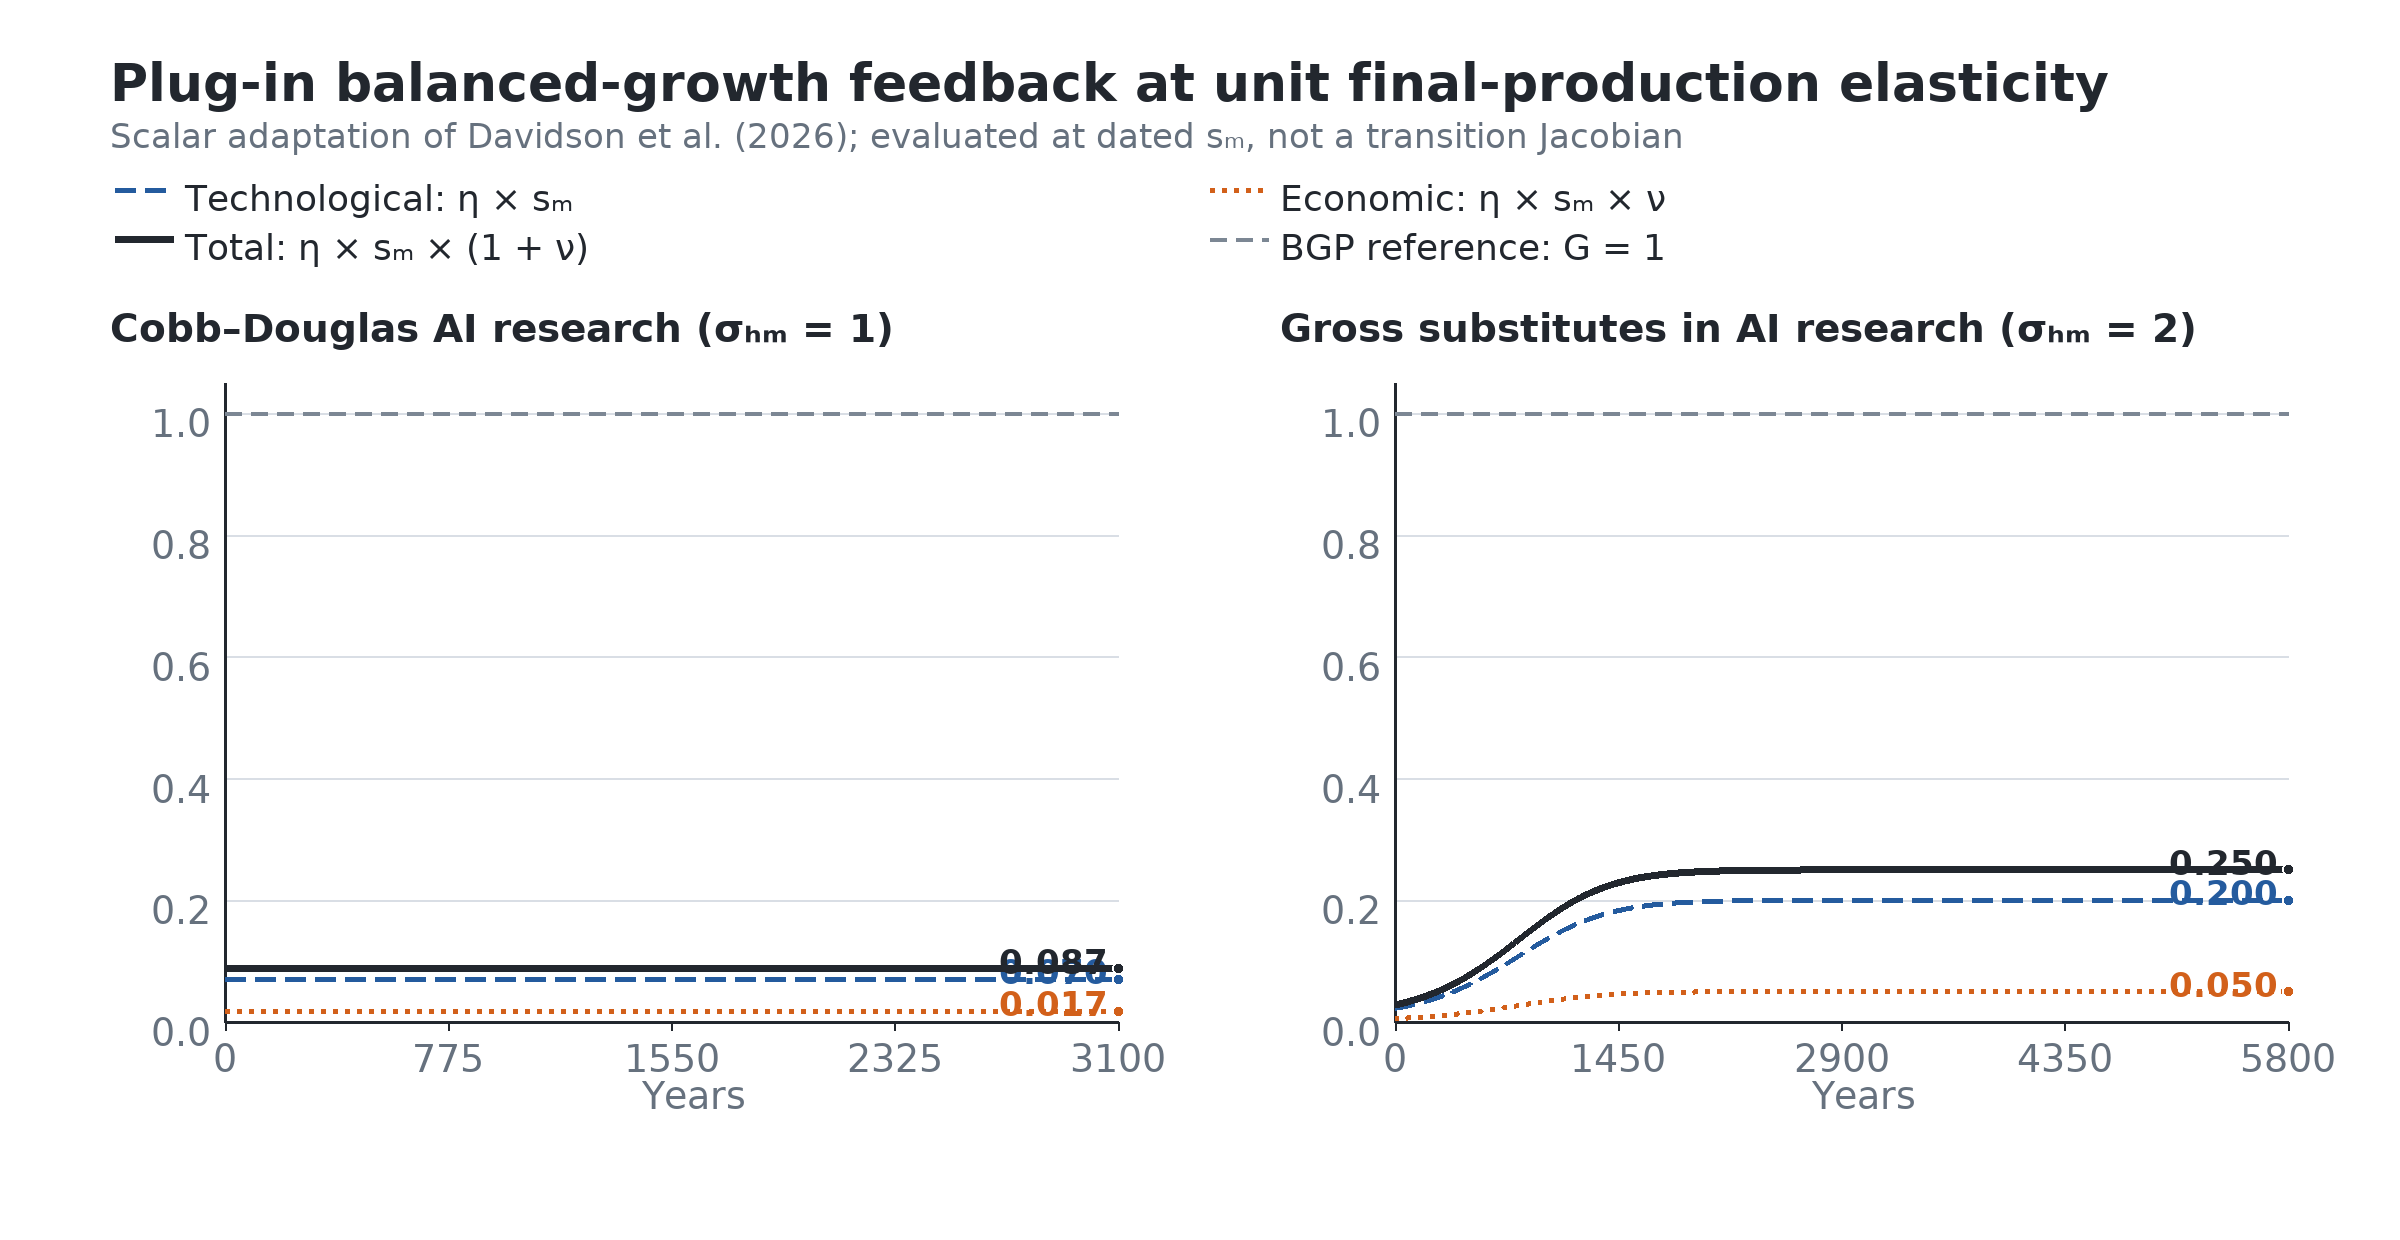
\includegraphics[width=\textwidth]{figures_axm/axm_unit_elasticity_feedback_diagnostic.png}
\caption{Plug-in balanced-growth feedback accounting evaluated at \(s_M(t)\)
along the two unit-elasticity finite-horizon candidate paths. The construction is
a scalar adaptation of \citet{davidsonetal2026}, not the dated feedback Jacobian.
The horizontal line at one is the critical value for the balanced-growth
accounting in equation~\eqref{eq:axm-feedback-matrix}, not a sufficient condition
for explosive equilibrium dynamics.}
\label{fig:axm-feedback-diagnostic}
\end{figure}

\subsection{Acceptance tests, independent audits, and limits of the evidence}

For every reported unit-elasticity path and every horizon-robustness path, the
canonical code recomputes the dated static allocation and records the technology,
goods-market, labor-market, monopoly, research, and dynamic residuals. It also
checks the monopoly second-order condition and stores all six horizon paths,
rather than retaining only their initial jumps. The row-by-row audit reconstructs
\(X=AU\), the service \(AM\), the CES research-input index, the capability law,
both research first-order conditions, and the costate term
\(-\eta s_M\dot A/A\). The collocation derivative, rather than a plotted finite
difference, is used for the unit-elasticity dynamic residuals.

Table \ref{tab:axm-residuals} reports the solver-side diagnostics for the two
baseline unit-elasticity paths. Static identities and first-order conditions have
errors below \(10^{-10}\) in the stored solver diagnostics. The larger entries are
collocation residuals in the differential equations and remain close to
\(10^{-5}\).

\begin{table}[H]
\centering
\small
\caption{Unit-elasticity path diagnostics}
\label{tab:axm-residuals}
\begin{tabular}{lcc}
\toprule
Diagnostic & \(\sigma_{HM}=1\) & \(\sigma_{HM}=2\)\\
\midrule
Maximum goods-market residual & \(2.2\times10^{-16}\) & \(3.3\times10^{-16}\)\\
Maximum labor-market residual & \(3.6\times10^{-15}\) & \(7.1\times10^{-15}\)\\
Maximum technology log error & \(1.4\times10^{-14}\) & \(2.4\times10^{-12}\)\\
Maximum factor-price error & \(1.8\times10^{-15}\) & \(7.1\times10^{-15}\)\\
Maximum research-duality error & \(1.8\times10^{-14}\) & \(4.9\times10^{-11}\)\\
Maximum monopoly-FOC log error & \(1.6\times10^{-14}\) & \(2.7\times10^{-14}\)\\
Maximum research-FOC log error & \(1.8\times10^{-14}\) & \(2.4\times10^{-11}\)\\
Maximum dynamic path residual & \(1.2\times10^{-6}\) & \(5.4\times10^{-6}\)\\
Maximum horizon-induced initial-jump range & \(2.6\times10^{-9}\) & \(7.4\times10^{-9}\)\\
Minimum monopoly second-order margin & 0.1160 & 0.1160\\
Absolute terminal capability-growth error & \(6.1\times10^{-7}\) & \(4.1\times10^{-9}\)\\
Absolute terminal per-capita-output-growth error & \(5.4\times10^{-8}\) & \(8.2\times10^{-10}\)\\
Terminal automated research-expenditure share & 0.3500 & 1.00000\\
Log household terminal-TVC proxy & -85.23 & -160.83\\
Log developer terminal-TVC proxy & -87.54 & -163.14\\
\bottomrule
\end{tabular}
\end{table}

The horizon-induced range is the larger of the ranges of \(\log C(0)\) and
\(\log q(0)\), measured in log points. The terminal growth errors are absolute
differences between annual rates expressed as decimals. Across all six horizon
paths, the largest reconstructed static-equation error is
\(4.9\times10^{-11}\). The largest differential-equation residual is
\(6.6\times10^{-6}\), and both imposed terminal-ratio errors are below
\(8.0\times10^{-8}\). Every saved quantity remains positive, and the monopoly
second-order margin is strictly positive.

The two TVC entries evaluate the expressions in equation~\eqref{eq:axm-tvc} at
the finite terminal date. Their finite magnitudes depend on normalization; only
convergence to zero is invariant. They are truncation diagnostics, not direct
verification of a limit as \(t\to\infty\). Under the analytical balanced-growth
continuation, if it exists, both objects decay at rate \(\rho-n>0\).

The complementary-input calculations have a separate auditor, which does not
import the solver. Its source is
\path{scripts/audit_axm_complements.py}. It
reconstructs the static equations from the saved rows and estimates the four log
derivatives with centered local polynomials. Acceptance requires small static and
dynamic residuals, positive and interior allocations, a positive monopoly
second-order margin, no active saved clipping or fallback, accurate imposed
terminal restrictions, convergence of non-imposed terminal quantities, and
stable initial jumps across horizons.
Across the two displayed \(T=4{,}500\) paths, the largest reconstructed static
error is \(5.32\times10^{-11}\), the largest independently differentiated
dynamic error is \(5.20\times10^{-7}\), and the largest monopoly first-order
condition error is \(3.14\times10^{-10}\). Across all six cold starts, the
largest solver root-mean-square residual is \(9.36\times10^{-7}\), the largest
independently differentiated dynamic error is \(8.35\times10^{-7}\), and the
largest horizon-induced initial-jump range is \(2.92\times10^{-7}\) log points.
Every prespecified acceptance gate
passes, including the finite-date transversality proxies. These proxies remain
truncation diagnostics and do not establish the infinite-horizon limits.

The high-substitution calculation is checked by
\path{scripts/audit_axm_high_sigma.py}. This auditor reconstructs all
technologies, prices, first-order conditions, income shares, the household
budget, market clearing, and the four dynamic right-hand sides without calling
the solver's static-equilibrium routine. It also differentiates the four
log-state paths independently on a compact calendar window. Acceptance requires positivity,
a strictly positive monopoly second-order margin, no active saved clipping,
small equation residuals, stable initial jumps, convergence on common calendar
and event-time windows, stability of the imposed terminal ratios, convergence of
the non-imposed terminal quantities, and stabilization of
\eqref{eq:axm-singularity-tail-estimate}. All prespecified gates pass for
\(z_T=16,32,64,128\).

\begin{sloppypar}
The simulation files and residual summaries are stored in
\path{numerical_axm}. The canonical fixed-horizon solver is
\path{scripts/simulate_axm_equilibrium.py}; the complementary-input runner and
the free-boundary solver are
\path{scripts/simulate_axm_complements_equilibrium.py} and
\path{scripts/simulate_axm_high_sigma_equilibrium.py}. The mapping from manuscript
equations to solver objects and diagnostics is stored in
\path{numerical_axm/equilibrium_equation_map.csv}. Scripts without the
\texttt{axm} designation that solve or simulate an equilibrium implement the
earlier research specification and do not generate evidence used in this paper.
Plotting scripts read accepted paths and do not solve an additional equilibrium
system. In particular,
\path{scripts/plot_axm_distribution_decomposition.py} verifies the hashes in
all three accepted audit manifests, reconstructs the six components of
\eqref{eq:axm-consolidated-distribution} from dated prices and quantities, and
checks nonnegativity and accounting closure before drawing the cross-regime
figure.
The reported reruns used Python 3.12.13, NumPy 2.5.2, SciPy 1.18.0, and Pillow
12.3.0. These versions are pinned in \path{requirements-numerical.txt}.
Floating-point arithmetic and platform-specific rendering can still prevent
bit-for-bit identity across computing environments; acceptance is based on the
reported numerical tolerances and equation audits rather than file identity
alone.
Within \path{numerical_axm}, diagnostic values and pass/fail status are stored in
\path{audit_report.csv}, \path{complements_acceptance_report.csv}, and
\path{high_sigma_sigma150_validated_acceptance_report.csv}. The last two reports
also state their numerical thresholds, and their manifests record the audited
inputs. Unit-elasticity thresholds are defined in
\path{scripts/audit_axm_model.py};
\path{unit_elasticity_audit_manifest.json} binds its four numerical inputs to
the current audit and generator scripts by SHA-256 hash.
\end{sloppypar}

Convergence of the collocation routine establishes only that a finite-horizon or
finite-boundary discretization satisfies its equations and imposed boundary
conditions within the reported tolerances. Agreement of an imposed terminal
ratio is not independent validation. The overidentifying evidence comes from the
dated residuals, non-imposed quantities, and stability across horizons or
boundaries. Finite terminal values of the two transversality expressions are
recorded, but they do not prove their infinite-horizon limits. The
unit-elasticity sufficiency result applies only to an admissible exact continuation
satisfying the full system and both transversality conditions. The
complementary-input calculations are finite-horizon approximations to candidate
paths. The
gross-substitutes calculations are finite-boundary approximations to a
conditional pre-singular branch of the necessary conditions; they do not establish
an infinite-horizon equilibrium, global stability, uniqueness, or reachability
from arbitrary initial states.

Table \ref{tab:axm-high-sigma-convergence} and Figure
\ref{fig:axm-high-sigma-ratios} report the free-boundary diagnostics removed from
the sequence of economic outcomes in the main text. Only \(C/Y\), \(qA/K\), and
terminal \(Y/K\) are imposed at each boundary. The other terminal quantities and
the agreement of overlapping path segments are overidentifying checks on the
conditional asymptotic characterization.

\begin{table}[H]
\centering
\small
\caption{Free-boundary convergence and terminal ratios,
\(\sigma_{XL}=1.5,\ \sigma_{HM}=2\)}
\label{tab:axm-high-sigma-convergence}
\begin{tabular}{lccccc}
\toprule
Terminal \(Y/K\) & 16 & 32 & 64 & 128 & Limit\\
\midrule
Estimated \(T^*\) & 1669.005 & 1669.021 & 1669.025 & 1669.026 & ---\\
\(g_A/(Y/K)\) & 0.02265 & 0.02296 & 0.02313 & 0.02322 & 0.02332\\
\(U/Y\) & 0.44889 & 0.44890 & 0.44890 & 0.44890 & 0.44890\\
\(M/Y\) & 0.03081 & 0.03123 & 0.03146 & 0.03159 & 0.03172\\
\((\dot K+\delta K)/Y\) & 0.28357 & 0.28315 & 0.28291 & 0.28279 & 0.28266\\
\(s_X\) & 0.999986 & 0.999998 & 1.000000 & 1.000000 & 1\\
\(wN/Y\) & \(9.37\times10^{-6}\) & \(1.65\times10^{-6}\) & \(2.91\times10^{-7}\) & \(5.16\times10^{-8}\) & 0\\
\bottomrule
\end{tabular}

\medskip
\parbox{0.94\textwidth}{\footnotesize \emph{Notes:} The estimated \(T^*\) is
measured in model time. All remaining entries are ratios expressed as fractions,
so, for example, 0.02265 corresponds to 2.265 percent. The final column reports
the conditional analytical limit.}
\end{table}

\begin{figure}[H]
\centering
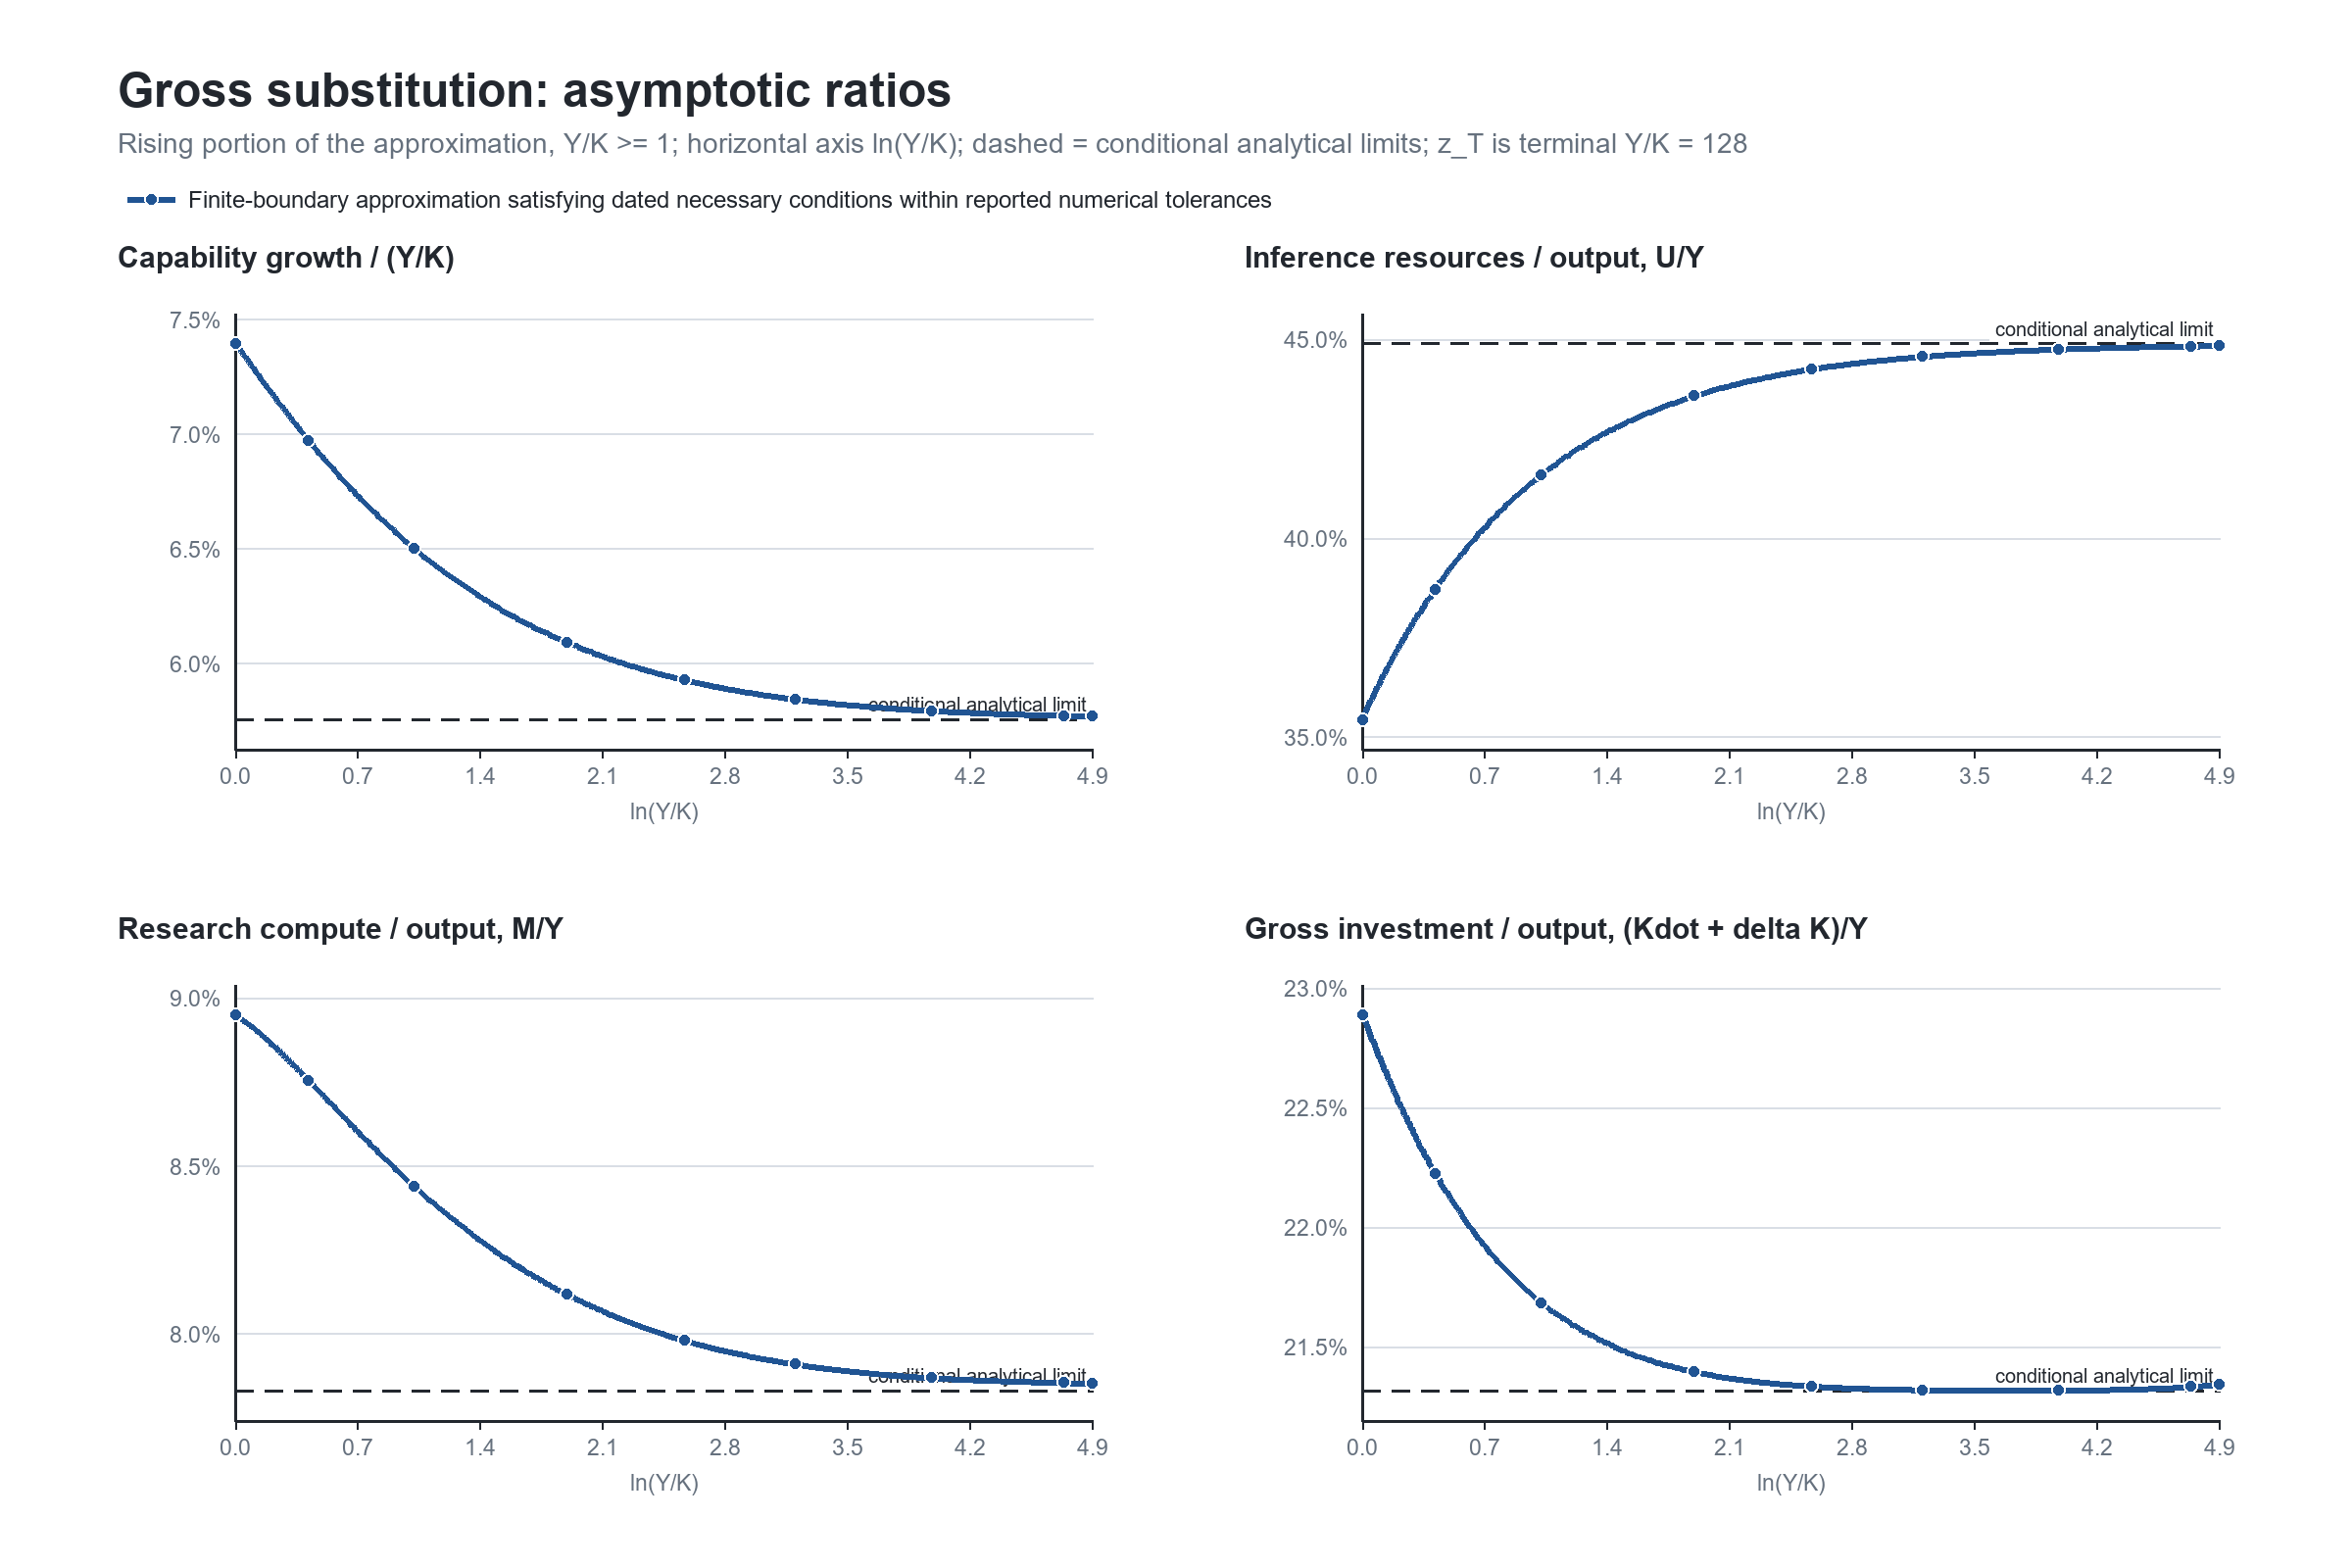
\includegraphics[width=\textwidth]{figures_axm/high_sigma_validated_asymptotic_ratios.png}
\caption{Selected non-imposed ratios along the rising branch of \(Y/K\). The
horizontal axis is \(\ln(Y/K)\); dashed lines are the conditional analytical
limits in Conditional Result \ref{prop:axm-singular-limit}. Vertical axes use
linear percentages with panel-specific ranges.}
\label{fig:axm-high-sigma-ratios}
\end{figure}

\begin{figure}[H]
\centering
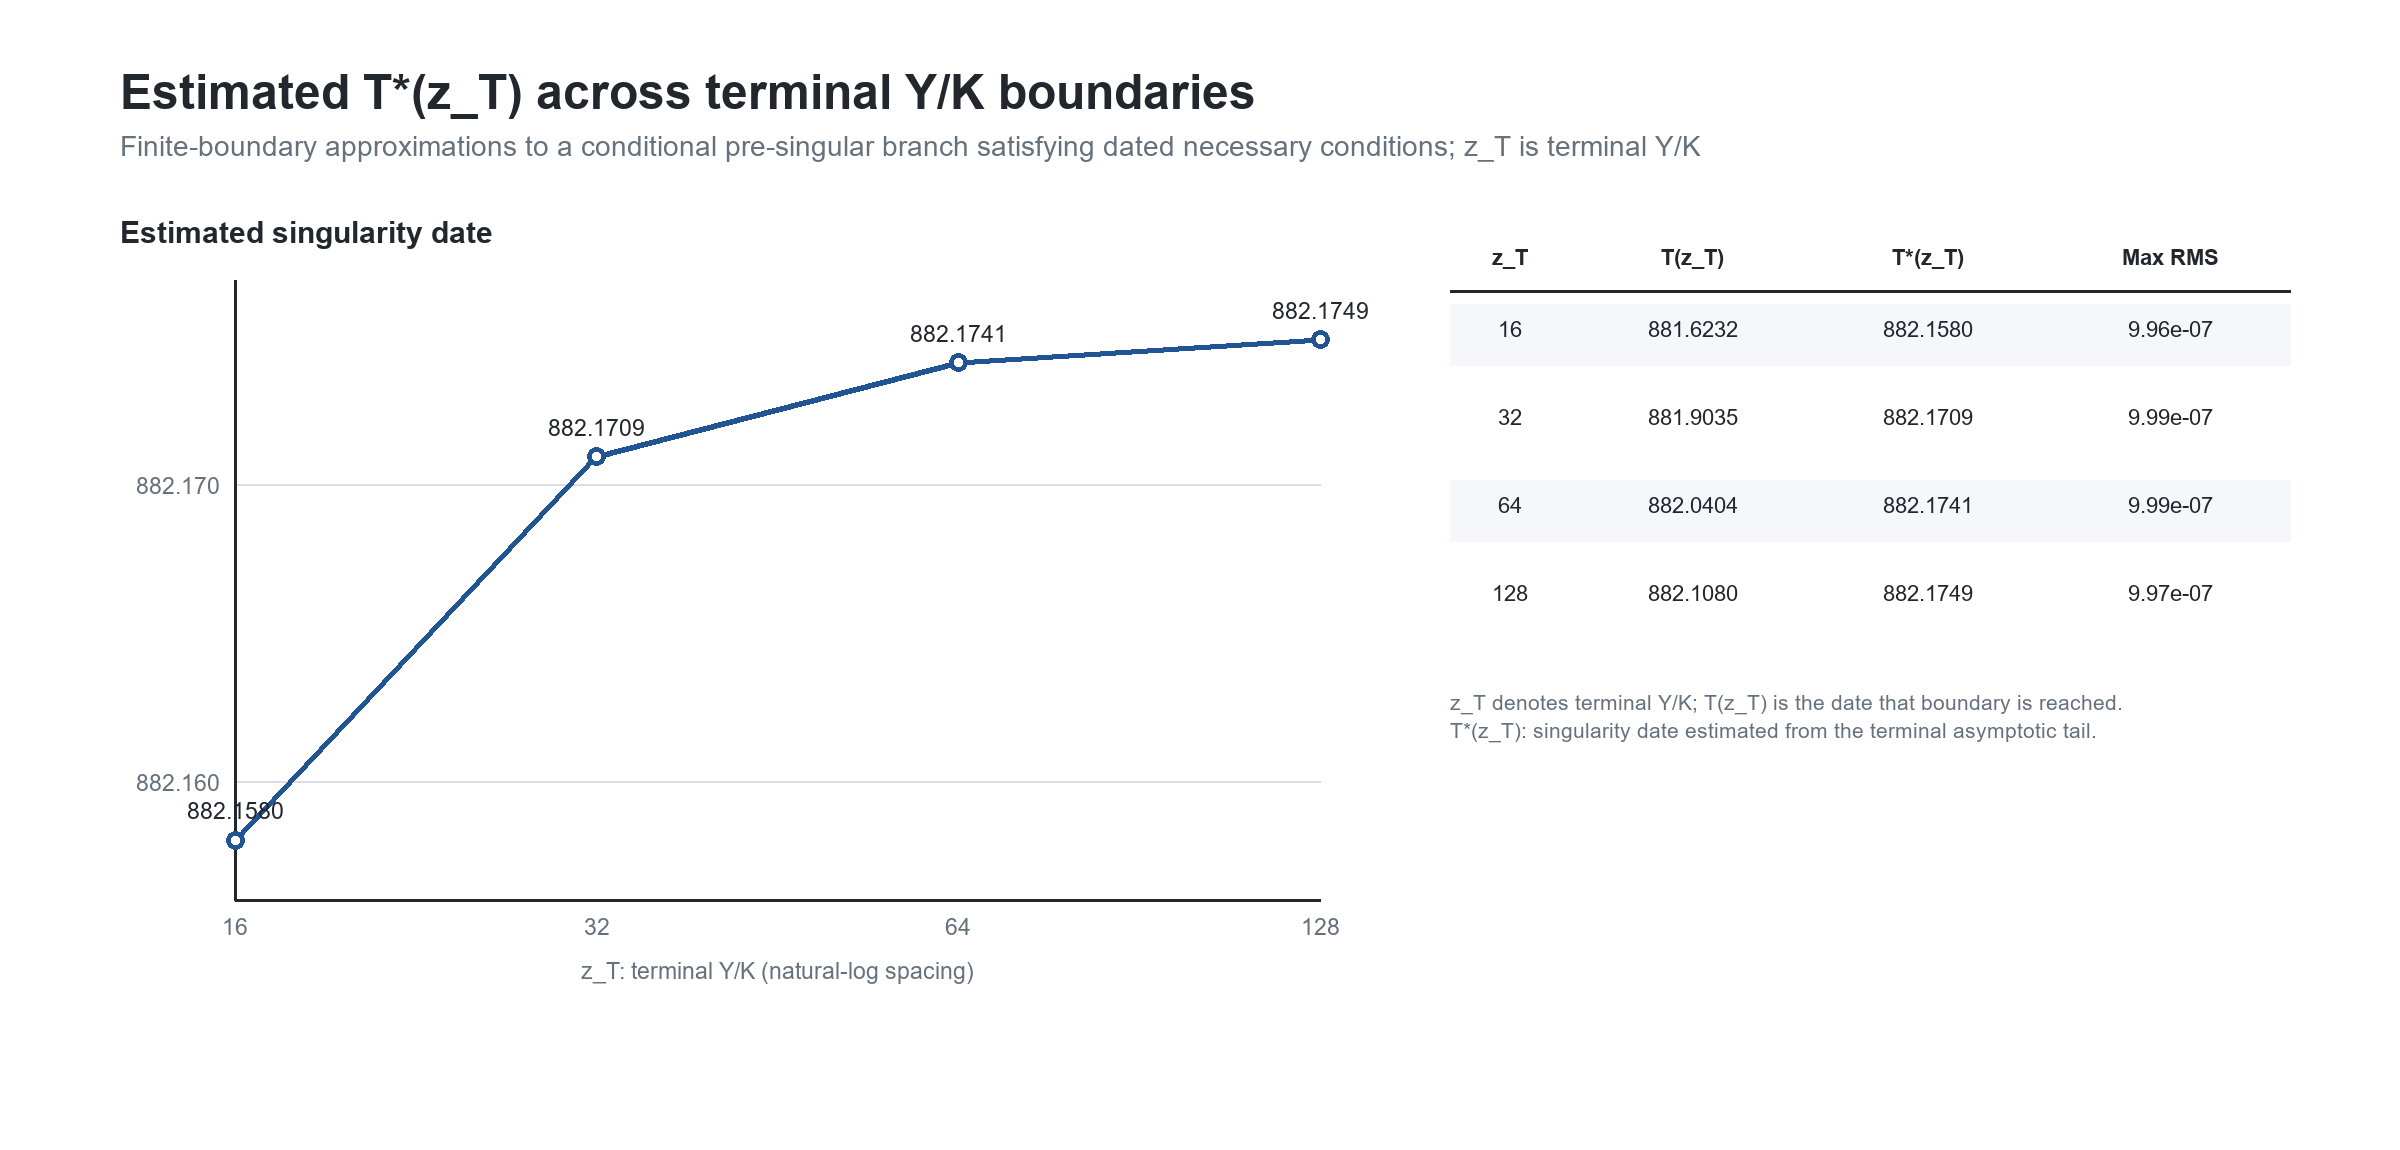
\includegraphics[width=\textwidth]{figures_axm/high_sigma_validated_boundary_convergence.png}
\caption{Free-boundary convergence diagnostic, where
\(z_T\equiv(Y/K)(T)\). \(T(z_T)\) is the date at which the approximation reaches
its artificial terminal boundary. The graphic writes \(T^*(z_T)\) for the tail
estimate \(\widehat T(z_T)\) in
\eqref{eq:axm-singularity-tail-estimate}. The residual column reports the maximum
collocation root-mean-square error.}
\label{fig:axm-high-sigma-boundary-convergence}
\end{figure}


\bibliographystyle{apalike}
\bibliography{references}

\end{document}
